% $Id: doku.tex,v 1.25 2010/08/10 08:18:00 baum Exp $
% Tag $Name: tinyheb-1-6-3 $


% Copyright (C) 2004 - 2013 Thomas Baum <thomas.baum@arcor.de>
% Thomas Baum, 42719 Solingen, Germany

% This program is free software; you can redistribute it and/or modify
% it under the terms of the GNU General Public License as published by
% the Free Software Foundation; either version 2 of the License, or
% (at your option) any later version.

% This program is distributed in the hope that it will be useful,
% but WITHOUT ANY WARRANTY; without even the implied warranty of
% MERCHANTABILITY or FITNESS FOR A PARTICULAR PURPOSE.  See the
% GNU General Public License for more details.

% You should have received a copy of the GNU General Public License
% along with this program; if not, write to the Free Software
% Foundation, Inc., 59 Temple Place - Suite 330, Boston, MA 02111-1307, USA.


\documentclass [a4paper,totoc] {scrreprt}
%\documentclass [a4paper,bibtotoc,oneside] {scrbook}
%\documentclass [a4paper] {report}
%\setlength\parindent{0pt}
\usepackage{makeidx}
\usepackage{lmodern}
\usepackage{mathptmx} 
%\usepackage {times}
\title {\textit{tinyHeb}\/ Dokumentation\\Version 1.3.0}
\author {Thomas Baum\\Solingen\\Germany}
\date {Copyright \copyright \today}
\usepackage {ngerman}
\usepackage [T1]{fontenc} 
\usepackage [utf8] {inputenc}
\usepackage {array} 
\usepackage [german]{varioref}
\usepackage [pdftex]{graphicx}
\usepackage {tabularx}
\usepackage {supertabular}
\usepackage {caption}
%\usepackage [dvips]{graphicx}
\usepackage {paralist}
\usepackage {float}
%\usepackage {perpage}
%\MakePerPage{footnote}
\graphicspath{{./jpg/}}
%\DeclareGraphicsRule{*}{jpg}
\DeclareGraphicsExtensions{.pdf,.jpg,.ps}
%
% selbst definierte Befehle
\newcommand\knopf[1]{\texttt{#1}}
\newcommand\feld[1]{\textsc{#1}}
\newcommand\myHeb{\textit{tinyHeb}{}\/}
\newcommand\tinyHeb{\textit{tinyHeb}{}\/}
\makeindex
\usepackage {hyperref}
\begin{document}
\nocite{*}
\maketitle[1]
\begin {abstract}
In diesem Dokument sind die Funktionsweise des Programmes \tinyHeb,
die Entstehungsgeschichte und Installationshinweise beschrieben.

Das Programm ist freie Software. Sie können es unter den Bedingungen der GNU
General Public License, wie von der Free Software Foundation veröffentlicht,
weitergeben und/oder modifizieren, entweder gemäß Version 2 der Lizenz oder
(nach Ihrer Option) jeder späteren Version.

Die Veröffentlichung dieses Programms erfolgt in der Hoffnung, dass es Ihnen
von Nutzen sein wird, aber OHNE IRGENDEINE GARANTIE, sogar ohne die implizite
Garantie der MARKTREIFE oder der VERWENDBARKEIT FÜR EINEN BESTIMMTEN ZWECK.
Deteils finden Sie in der GNU General Public License.

Für Fehler in diesem Handbuch oder Fehler die aus der Benutzung des
Handbuches entstehen, wird keine Haftung übernommen.
\end {abstract}
\tableofcontents

%\frontmatter

\chapter{Entstehungsgeschichte\label{entstehungsgeschichte:kap}}
Wie bei fast allen anderen Hebammenabrechnungsprogrammen, war auch hier die Lebenspartnerin Auslöser.
Im November 2003 erstellte meine Freundin\footnote{seit dem 20.05.06 ist meine Freundin nicht mehr meine Freundin, sondern meine Frau}
ihre Abrechnungen gegenüber den Krankenkassen
immer noch auf Papiervordrucken. Wie man sich leicht vorstellen kann,
führte das u.a. bei der Berechnung des Kilometergeldes und der Ermittlung des
Wochentages zu Problemen. Die Wochentage sind natürlich nur dann ein
Problem, wenn man die Rechnung erst Wochen oder gar Monate nach der 
Leistungserbringung schreibt. Auch ist die Berechnung der Dauer bei 
bestimmten Leistungen, wie z.B. Hilfe bei Schwangerschaftsbeschwerden
zeitaufwendig, weil gerechnet werden muss.

Naheliegend war natürlich, entweder ein Programm zu kaufen oder auf Freeware
zurückzugreifen. Auf dem Markt waren zu diesem Zeitpunkt zwei Programme 
erhältlich.
Leider sind beide Programme nicht für Linux erhältlich. 
Also musste selber ein Programm geschrieben werden, so entstand \tinyHeb.

\section{erster Versuch}
Im November 2003 ging es an die Konzeptionierung, Datenstrukturen und
Datenbanktabellen wurden designed. Die Spezifikation der Anforderungen 
durch meine Freundin gestaltete sich dabei recht schwierig, da sie zu
diesem Zeipunkt ca. 500 Km von mir entfernt wohnte.
Trotzdem enstanden mit HTML und perl erste Masken, in denen Stammdaten
und Abrechnungsdaten erfasst werden konnten.

Das Ergebnis entsprach leider überhaupt nicht den Anforderungen meines
``Kunden''. Es sollte eigentlich alles genauso sein, wie auf den
Papiervordrucken, nur dass jetzt Gesamtsummen, das Wegegeld und die Zeiten
automatisch berechnet werden sollten. Auch die entgültige Rechnung sollte
genauso aussehen, wie bei den Papierrechnungen\footnote{Das ist nach Meinung des Authors typisch für Softwareentwicklungsprojekte, bestehende Prozesse sollen sich nicht ändern.}.
Da mir solche Anforderungen von der Arbeit her bekannt waren und ich privat 
nicht die gleichen Diskussionen führen wollte, die ich beruflich führen muss,
wurde die Entwicklung im März 2004 eingestellt. Zum Glück habe ich nicht
alle Daten gelöscht, sondern sie verblieben im CVS Repository.

\section{zweiter Versuch}
Im März 2005 stellte meine Freundin ``plötzlich'' fest, dass ihre
Papierabrechnungen nicht mehr von den Krankenkassen akzeptiert werden.
Sie wollte jetzt ein kommerzielles Programm kaufen. Der Preis
erschien mir sehr teuer und ich war mir nicht sicher, ob die ganze Sache
mit wine auch wirklich unter Linux läuft.

Die Evaluierungsphase war dann recht kurz. Mit qemu und einer Win95
Installation konnte getestet werden und welche Überraschung, die Erfassung
und auch der Rechnungsdruck sahen so aus, wie ich mir das im März 2004
vorgestellt hatte.
Also ging die Entwicklung an der Stelle weiter wo ich 2004 aufgehört hatte.
Es konnten wesentliche Teile der Software wiederverwendet werden. Inbs.
die Zugriffsroutinen auf die Datenbank, die Erfassungsmaske für die 
Frauenstammdaten und Feiertage.

\section{dritter Teil}
Anfang Oktober 2005 überraschte mich meine Freundin mit der Nachricht, dass
ab Januar 2006 die Abrechnungen elektronisch an die Krankenkassen zu melden
sind. Super, gerade hatte ich wesentliche Teile der Software fertig und
jetzt elektronischer Datenaustausch. Also ging es am 03.10.2005 daran
die Spezifikation für den Datenaustausch per E-Mail zu besorgen. Die
komplette Spezifikation \cite{richtliniendatenaustausch},\cite{anlage1}
füllt ca. einen Aktenordner. Leider ist es wie bei
vielen Spezifikationen, es bleiben einige Fragen offen. Diese Fragen wurden
mir vom RZ der AOK Rheiland beantwortet. Den Kollegen an dieser Stelle
meinen ausdrücklichen Dank, sonst hätte ich es wohl nie geschafft. Mitte
Oktober war es möglich, die ersten Rechnungen im Edifact Format zu generieren.
Das ist für den Datenaustausch natürlich nicht ausreichend, da die Daten
verschlüsselt werden müssen. Die Verschlüsselung wurde zum größten Problem
im Rahmen der Entwicklung. Insb. bei der Kommunikation mit dem Rechenzentrum
wurden gleiche Begriffe unterschiedlich interpretiert. Ende Oktober 2005
war das Problem dann klar, die Daten müssen PKCS\#7 verschlüsselt werden.
Die AOK war aber erst ab November in der Lage Daten, die mit PKCS\#7
verschlüsselt wurden wieder zu entschlüsseln. Ab Januar 2006 konnten endlich
echte Daten in der Erprobungsphase ausgetauscht werden und heute (Juni 2008)
sind alle Datenannahmestellen an die Software angeschlossen.
Die Zertifizierung der AOK Rheinland liegt seit dem 12.05.2006, die
des ARZ-Emmendingen seit dem 29.08.2006 und der AOK Bayern seit dem
05.06.2007 vor. Bei anderen Datenannahmestellen hat es meine Frau noch nicht
bis zum Echtbetrieb geschafft, das liegt aber vor allem daran, dass zu
wenig Rechnungen an die entsprechenden Datenannahmestellen geschickt werden
oder die Datenannahmestelle selbst noch nicht in der Lage ist Rechnungen
im Echtbetrieb entgegen zu nehmen.

Falls es Problem mit dem Datenaustausch unter \tinyHeb\/ geben sollte,
hängen diese in der Regel mit der eigentümlichen Verarbeitung einzelner
Datenannahmestellen zusammen, insb. bei verschlüsselten und signierten 
Rechnungen.

An dieser Stelle soll nicht auf alle
Probleme, die es mit dem Anschluss einer Datenannahmestelle gibt eingegangen
werden. Im Kapitel \vref{parameter:kap} wird im Detail beschrieben, welche
Einstellungen vorzunehmen sind. Weiterhin wird im Anhang
\vref{anhang:elekrech} aufgezeigt, wie man besonders
schnell zum Datenaustausch zugelassen wird, und warum das ganze nichts
kostet.

\section{Über dieses Handbuch}
Um mit \tinyHeb\/ arbeiten zu können, ist es nicht notwendig, das Handbuch
komplett
von vorne nach hinten zu lesen. Das Handbuch soll eher als Nachschlagewerk
dienen, wenn man an der einen oder anderen Stelle ein Problem hat.

Trotzdem ist es notwendig, einige Kapitel des Handbuches zu lesen, wenn
man mehr als ``Spielrechnungen'' produzieren möchte. 

Eine kurze Zusammenfassung der Kapitel soll das Auffinden der für den
Leser/ Leserin wesentlichen Teile erleichtern.

\paragraph{}
In Kapitel \ref{entstehungsgeschichte:kap}, 
\textit{Entstehungsgeschichte} sind die Motivation für 
\tinyHeb\/, aber auch die Probleme, die mit der 
Entwicklung von \tinyHeb\/ verbunden waren, beschrieben.
\paragraph{}

In Kapitel \ref{installation:kap}, \textit{Installation} finden sich 
Hinweise zur Installation von \tinyHeb\/ aus den Sourcen. Falls man
\tinyHeb\/ mit Hilfe der RPM Pakete installiert hat, ist es nicht
notwendig das gesamte Kapitel zu lesen. Statt dessen kann man direkt 
bei Abschnitt \ref{einleitung:parameter:kap}, \textit{Parameter} mit
dem Lesen beginnen. Dort ist u.a. beschrieben, wie Name, Anschrift,
IK-Nummer der Hebamme, usw. in \tinyHeb\/ hinterlegt werden, aber auch wie 
eingestellt wird, dass nach der korrekten Gebührenordnung abgerechnet wird.
\paragraph{}

In Kapitel \ref{Kurzanleitung}, \textit{Kurzanleitung} sind die
wesentlichen Schritte beschrieben, um mit \tinyHeb\/ schnell eine
Rechnung zu produzieren. Dieses Kapitel sollte gelesen werden.
\paragraph{}

In Kapitel \ref{anleitung}, \textit{Anleitung} sind alle Details,
Masken, Plausibilitätenprüfungen, usw. von \tinyHeb\/ beschrieben. 
Dieses Kapitel muss nicht in gänze gelesen werden, hilft aber weiter, wenn man
alle Features des Programms nutzen möchte. Es eignet sich insb. als
Nachschlagewerk, wenn es Probleme geben sollte.
\paragraph{}

In Kapitel \ref{parameter:kap}, \textit{Parameter} sind alle
Parameter beschrieben, die es in \tinyHeb\/ gibt. Wichtig sind dabei
der Abschnitt \ref{parm:heb:abs}, \textit{Angaben zur Hebamme},
Abschnitt \ref{datenannahmestellen:abs}, \textit{Datenannahmestellen}
und der Abschnitt \ref{feiertage:abs}, \textit{Feiertage}.

Im Abschnitt \textit{Angaben zur Hebamme} sind alle Daten zur
Hebamme beschrieben, die wichtig sind, um eine korrekte Rechnung zu
produzieren.

Im Abschnitt \textit{Datenannahmestellen} sind alle Parameter
beschrieben, die für den elektronischen Datenaustausch benötigt werden.
Wie eine neue Datenannahmestelle parametrisiert werden muss und welche
Werte zu ändern sind, wenn man z.B. von der Erprobungsphase in den 
Echtbetrieb wechselt.

Im Abschnitt \textit{Feiertage} wird gezeigt, wie neue Feiertage
in \tinyHeb\/ eingepflegt werden können.
\paragraph{}

Im Anhang in Kapitel \ref{anhang:elekrech}, 
\textit{Anmeldung zum E-Mail Verfahren}
findet sich eine Beschreibung, wie man bei den einzelnen Krankenkassen
zum elektronischen Abrechnungsverfahren zugelassen wird. Dieser Abschnitt
sollte gelesen werden, wenn man Rechnungen elektronisch verschicken möchte.
\paragraph{}

Im Anhang in Kapitel \ref{anhang:aktkk}, 
\textit{Aktualisierung der Krankenkassendaten} ist
beschrieben, wie sich die Anschriftendaten auf Basis der Kostenträgerdateien
aktualisieren lassen. Dieser Abschnitt muss erst am Ende eines Quartals
gelesen werden oder wenn man sich wundert, warum eine Krankenkasse in 
\tinyHeb\/ nicht existiert, bzw. die Rechnung von der Krankenkasse mit
dem Vermerk ``wir sind nicht zuständig'' abgelehnt wird.
\paragraph{}

Im Anhang in Kapitel \ref{anhang:provider},
\textit{zusätzliche Provider im elektronischen
Datenaustausch} wird gezeigt, wie \tinyHeb\/ parametrisiert werden muss, damit
E-Mails über den Internet-Provider verschickt werden können und wie vorzugehen
ist, wenn mehr
als ein E-Mail Provider benötigt wird. Windows Nutzer sollten dieses
Kapitel in jedem Fall lesen, unter Linux ist das Kapitel nur notwendig,
wenn es Probleme mit dem E-Mail Versand der Rechnung gibt.
\paragraph{}

Im Anhang in Kapitel \ref{anhang:eigenes_cert},
\textit{Ein eigenes Zertifikat} befindet sich die Beschreibung,
wie eine Zertifikatsanfrage generiert wird und das Zertifikat in
\tinyHeb\/ eingebunden wird. Ein solches Zertifikat wird für den 
Datenaustausch bei einigen Datenannahmestellen\footnote{u.a. Inter-Forum Systems, Syntela und Medent} \index{Datenannahmestellen}
benötigt.
\paragraph{}

Bei meiner Frau und mir gibt es folgende Arbeitsteilung bzgl. der
Rechnungen. Meine Frau erfasst die Rechnungen, ich bin für die
Parametrisierung des Programms und die Kommunikation mit 
den Datenannahmestellen
zuständig. Sollte dies bei Euch so ähnlich sein, gilt folgender Tipp
für die Arbeit mit dem Handbuch: Die Hebamme sollte das Kapitel 
\ref{anleitung}, \textit{Anleitung} lesen, ihr Mann/ Lebensgefährte/
Freund die anderen oben
als wichtig gekennzeichneten Kapitel.


\section{Danksagungen}
Wie in jedem Handbuch soll auch hier dieses Kapitel nicht fehlen. Ohne
Hilfe wäre \tinyHeb\/ nicht das geworden, was es heute ist.

Besonders bedanken muss ich mich natürlich bei meiner Frau Marlies, die
sehr viel Geduld mit mir hat, insb. wenn ich 
viele Stunden vor dem Rechner sitze, weil ich neue Funktionalitäten
einbaue oder ich mich mit den Fragen und Problemen
der Nutzer und Nutzerinnen beschäftige.
Abgesehen davon, war sie die erste Nutzerin und testet auch heute noch die
Anwendung als erste. Auf viele Plausibilitätenprüfungen wäre ich ohne
ihre Hilfe nicht gekommen.

Dann sind die Mitarbeiter des RZ der AOK Rheinland zu erwähnen,
die mir sehr freundlich viele Fragen beantwortet haben. Namentlich sind
dies die Herren B. und Z.

Mit dem ARZ-Emmendingen habe ich alle Konstellationen der Verschlüsselung
und Signierung getestet. Ich bin jedesmal begeistert, wie schnell und
freundlich auf Fragen reagiert wird. Hier sind die Herren G. und S.
besonders zu erwähnen.

Die Leser der Newsgroup \verb|de.comp.os.unix.linux.misc| haben mich dazu
gebracht \tinyHeb\/ überhaupt zu veröffentlichen. Darunter war u.a.
Rolf aus Jülich.

Rolf und seine Frau waren die ersten Nutzer überhaupt, die
beiden mussten die meisten Fehler aushalten, da sie \tinyHeb\/ schon
seit März 2006 benutzen.

Heiner aus Hannover war einer der ersten Windows Nutzer (wenn nicht der
Erste) und hat die Installationsanleitung für Windows geschrieben.

Katrin hat mich auf wesentliche Fehler des setups unter Windows Vista 
hingewiesen\footnote{das Stand Juni 2008 immer noch alles andere als
perfekt ist} und als Alpha Testerin fungiert.

Es gibt noch viele weitere zu erwähnen, wie z.B. Bernhard, der
unermüdlich mit Krankenkassen und Datenannahmestellen telefoniert. Aber
irgendwann muss es auch mit den Danksagungen gut sein.

Last but not least gilt mein Dank allen Nutzern und Nutzerinnen, 
die mich auf
Fehler in der Anwendung hingewiesen und Verbesserungsvorschläge gemacht
haben. Ohne Euch wäre die Anwendung nicht das, was sie heute ist.

%\section{verwendete Konventionen}


%\mainmatter

\chapter{Installation\label{installation:kap}}
Für die Installation auf einem Linux Rechner sind einige Komponenten
Vorraussetzung. Diese sollten aber in jeder Distribution vorhanden sein.
Die hier vorliegene Beschreibung bezieht sich auf SuSE
Linux, sollte aber bei jeder anderen Distribution ähnlich funktionieren. 
Eine Installation auf einem Windows \index{Windows} System ist problemlos 
möglich und ausführlich in \cite{installation_windows} beschrieben.

\begin{itemize}
\item Ein Webserver, z.B. Apache
\item perl
\item mysql
\item ghostview (gv) um sich die Rechnungsvorschau im Browser anzusehen
\item OpenSSL, wenn elektronischer Datenaustausch gewünscht ist.
\end{itemize}
%
\section {Kopieren der Scripte}
Nachdem man den Tar-Ball aus dem Internet geladen und entpackt hat, müssen
die Scripte noch an die ``richtige'' Stelle kopiert werden. Dazu
einfach als root \verb|make install| eingeben. Danach ist es nur noch 
notwendig fehlende Perl Module zu installieren und die Datenbank
zu initialisieren. Dies ist in den nachfolgenden Abschnitten beschrieben.

\section {Anpassen Apache Konfiguration}
Die Apache \index{Apache} Konfiguration wird durch das 
Makefile \index{Makefile} automatisch an die
richtige Stelle im Verzeichnisbaum kopiert. Danach ist ein Neustart
des Webservers notwendig. Wer die Anpassung per Hand vornehmen möchte,
muss wie unten beschrieben vorgehen:
\begin {enumerate}
%\item Das Modul \verb|mod_perl.so| muss geladen werden, dies kann über Yast gemacht werden.
\item Kopieren der Datei \verb|tinyheb.conf| aus dem Verzeichnis apache2\\
nach \verb|/etc/apache2/conf.d/|
\item den Apache Server mit \verb|rcapache2 restart| (SuSE Linux) oder\\
\verb|sudo /etc/init.d/apache2 restart| (Debian) neu starten.
%\begin{verbatim}
%Alias /tinyheb/  ''/srv/www/cgi-bin/tinyheb/''
%\end{verbatim}
%
%\item Setzen der Direktiven in der Datei /etc/apache2/default-server.conf
%\begin{verbatim}
%<Directory /srv/www/cgi-bin/tinyheb>
%        AllowOverride None
%        Options -Indexes +ExecCGI +FollowSymLinks
%        AddHandler cgi-script pl
%        Order allow,deny
%        Allow from all
%</Directory>
%\end{verbatim}
\end {enumerate}
%
%\pagebreak[4]
\section{Perl}
Es werden einige Perl \index{Perl} Module benötigt, die ggf. nicht 
installiert sind.
Die meisten dieser Module sollten in der Distribution enthalten sein. Ansonsten
über den entsprechenden Paketmanager oder bei CPAN herunterladen.
\begin {enumerate}
\item DBI\index{DBI}
\item Date::Calc\index{Date::Calc}
\item CGI\index{CGI}
\item PostScript::Simple\index{PostScript::Simple}
\item File::stat und MIME::QuotedPrint falls elektronische Rechnungen
gewünscht sind.
\item Tk, Tk::BrowseEntry, Tk::HList, Tk::ItemStyle, Mail::Sender, falls
die elektronischen Rechnungen mit grafischer Oberfläche verschickt werden
sollen.
\item Crypt::OpenSSL::X509 (optional) für eine verbesserte Performance beim
Einlesen von Zertifikaten.\index{Crypt::OpenSSL::X509}
\end {enumerate}
%
\section {MySQL}
Auch MySQL \index{MySQL} sollte in der Distribution enthalten sein, 
wenn noch nicht installiert, muss das nachgeholt werden. 
%Wichtig ist es einen Benutzer
%anzulegen, der Zugriff auf die benötigten Tabellen und die Datenbank hat.
%Hier gibt es verschiedene Tools (z.B. mysql-administrator) oder auch aus
%der Kommandozeile. Dieser Benutzer muss auf die Datenbank PRD\_Hebamme 
%zugreifen können und die Rechte haben Tabellen anlegen zu dürfen. Der
%Benutzer sollte wwwrun heissen, wenn man nicht die Datei Heb.pm anpassen
%möchte. In der aktuellen Version ist der Benutzer wwwrun ohne Passwort
%anzulegen, wer das nicht möchte, kann in der Datei Heb.pm das notwendige
%Passwort hinterlegen.

Im Verzeichnis DATA befindet sich ein SQL Script mit dem alle Tabellen
und ein technischer User mit den notwendigen Zugriffsrechten
angelegt und initialisiert werden: init.sql
\paragraph{}
Mit \verb|mysql -u root < init.sql| werden die nötigen Tabellen und der
technische Nutzer angelegt.

Bei einem Update der Software muss das Skript: \verb|update.pl|
ausgeführt werden
%
\section{Parameter\label{einleitung:parameter:kap}}
Jetzt müssen noch einige Parameter gepflegt werden, wie z.B. Name und 
Anschrift der Hebamme, dann kann die Arbeit wirklich losgehen.

Diese Parameter können direkt über die Konsole in der Datenbank geändert 
werden, oder aber über die Parameterpflege im Programm. Dazu ist es notwendig
\tinyHeb\/ zu starten. Man nimmt einen Webbrowser seiner Wahl\footnote{z.B. Firefox, Konqueror funktioniert nicht besonders gut} und ruft den Link
\nolinkurl{http://localhost/tinyheb/hebamme.html} im Browser auf.
Wenn alles funktioniert, bekommt man das Einstiegsbild (siehe Abbildung \vref{einstieg:fig}) zu sehen.
%
\begin{figure}[ht]
\centering
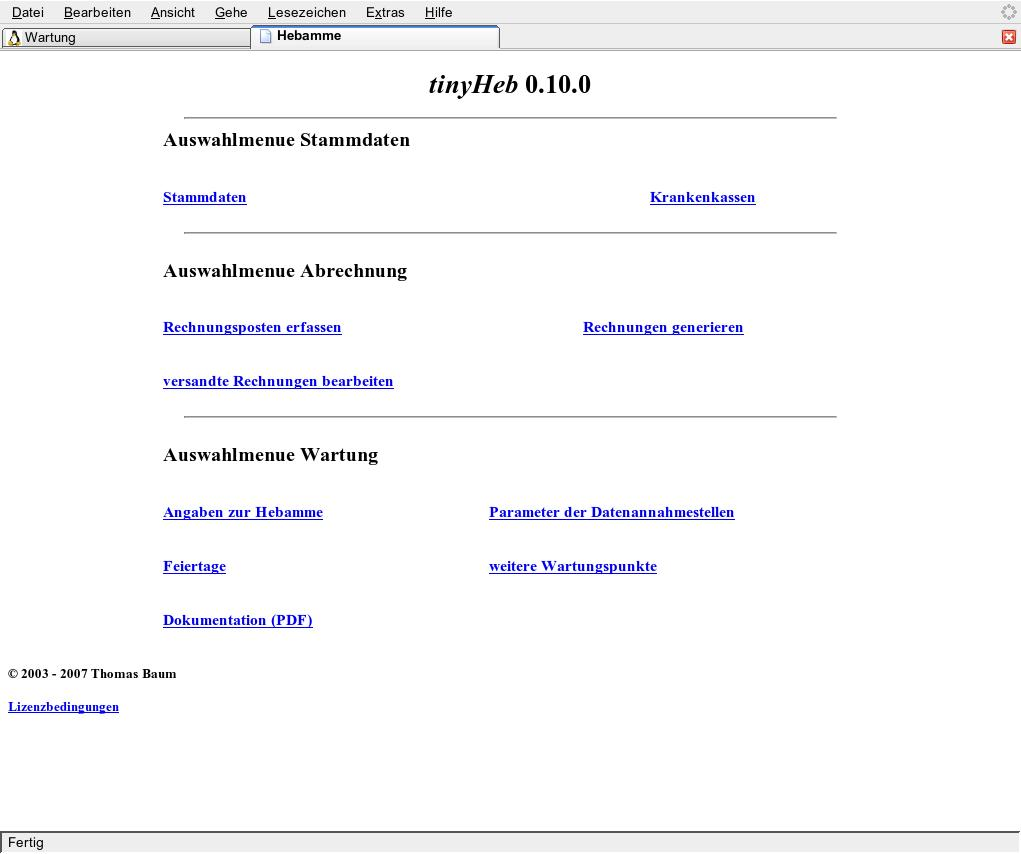
\includegraphics[width=80mm]{einstieg}
\caption{Einstiegsmenue in \emph{tinyHeb}\label{einstieg:fig}}
\end{figure}
%
Die Parameter die die Hebamme betreffen, können über die Maske
Angaben zur Hebamme gepflegt werden\footnote{Diese Maske steht erst seit
Release 0.9.0 zur Verfügung}. In diese Maske gelangt man aus dem
Hauptmenue über den Link \verb|Angaben| \verb|zur| \verb|Hebamme|.

Alternativ können die relevanten Parameter auch in der Maske Parameter
geändert werden.
Über den Link \verb|weitere| \verb|Wartungspunkte| gelangt man in das 
\tinyHeb\/ Wartungsmenue und von dort kommt man über den Link
\verb|alle| \verb|Parameter| in die Maske Parameter, hier können
Parameter neu erfasst, geändert und gelöscht werden. Eine genaue Beschreibung
dazu findet sich im Kapitel \vref{parameter:kap}.
Durch einen Klick auf den Knopf \texttt{Suchen}
 werden alle vorhandenen Parameter
angezeigt. Im konkreten Fall sind nur die Parameter von Interesse, die
mit HEB beginnen. Um nur diese angezeigt zu bekommen, erfasst man im Feld
\feld{Name} HEB -- alle anderen Felder müssen leer sein -- und klickt 
in diesem Fenster auf den Knopf \knopf{Suchen}. Als Ergebniss sollte das Bild 
aus Abbildung \vref{parameter:fig} erscheinen.
%
\begin{figure}[ht]
\centering
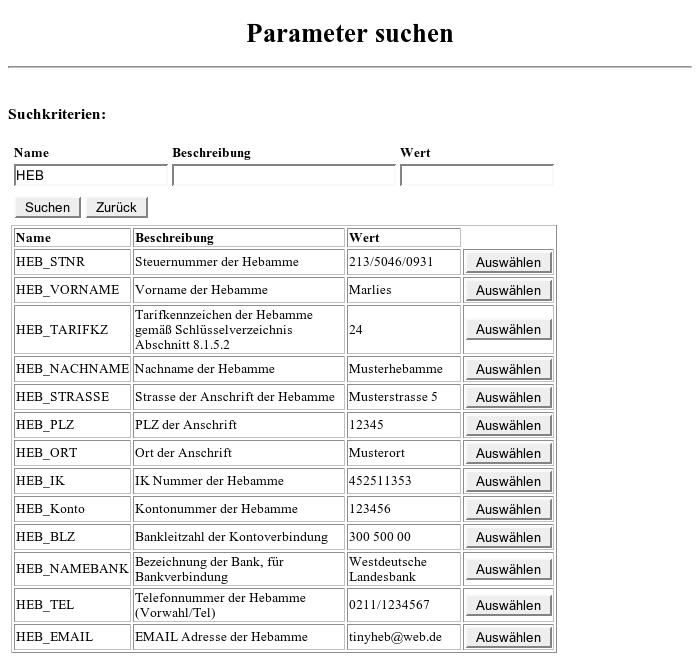
\includegraphics[width=80mm]{parameter_HEB}
\caption{Parameter Pflegemaske\label{parameter:fig}}
\end{figure}
%
Die in Tabelle \ref{parametertabelle:tab} angegebenen Parameter 
müssen angepasst werden.\\ 
Dabei ist unbedingt darauf zu achten, dass
die Parmeter Bezeichnung nicht aus Versehen geändert wird.
\marginline{\Huge\bfseries!}%
%
\begin{table}[ht]
\centering
\begin{tabular}{|ll|}
\firsthline
\textbf{Parameter Bezeichnung}&\textbf{Beschreibung Parameter}\\
HEB\_VORNAME&Vorname der Hebamme\\
HEB\_NACHNAME&Nachname der Hebamme\\
HEB\_STRASSE&Strasse der Anschrift der  Hebamme\\
HEB\_PLZ&PLZ der Anschrift der Hebamme\\
HEB\_ORT&Ort der Anschrift der Hebamme\\
HEB\_IK&IK Nummer der Hebamme\\
HEB\_Konto&Kontonummer zur Bankverbindung der Hebamme\\
HEB\_BLZ&Bankleitzahl der Bankverbindung\\
HEB\_NAMEBANK&Name der Bank\\
HEB\_TEL&Telefonnummer der Hebamme\\
HEB\_EMAIL&E-Mail Adresse der Hebamme im Format xy@provider.de\\
HEB\_STNR&Steuernummer der Hebamme im Format 123/4567/891\\
HEB\_TARIFKZ&Tarifkennzeichen: bundeseinheitlicher Tarif, West- oder\\
& Ostgebührenordnung, möglich sind 00 für bundeseinheitlich, 24 für West,\\ &
25 für Ost. Erfasst werden sollte immer 24 für West\\
HEB\_BUNDESLAND&Bundesland der Hebamme, entweder NRW, Bayern, Hessen, Hamburg,\\
& Rheinland-Pfalz, Thüringen, Sachsen, Sachsen-Anhalt, Niedersachsen,\\
& Brandenburg oder Baden-Würtemberg\\
HEB\_IK\_BELEG\_KKH&\index{Beleghebamme}IK Nummer des Krankenhauses, falls Beleghebamme\\
\lasthline
\end{tabular}
\caption{Parameter\label{parametertabelle:tab}}
\end{table}
%
\subsection{Feiertage}
Im weitesten Sinne gehören auch Feiertage zu den Parametern. Damit
diese korrekt bei Zuschlägen beachtet werden können, ist es notwendig
sie zu erfassen.
Wie schon bei den Parametern gelangt man aus dem Hauptmenue über den
Link \verb|Feiertage| in die Erfassungsmaske der Feiertage. Hier sind,
falls noch nicht vorhanden, alle Feiertage zu erfassen, für die man
Rechnungen erstellen möchte\footnote{Besser ist es mehr als weniger
Feiertage zu erfassen.}.
\\
Jetzt sollte alles Initialisiert sein und die Arbeit kann beginnen.
Falls etwas nicht gehen sollte, freue ich mich auf eine Mail:
thomas.baum@arcor.de

\subsection{Logo}
\index{Logo}
Auch das Logo der Hebamme gehört im weitesten Sinne zu den Parametern.
Wer möchte, dass ein Logo mit ausgedruckt wird, muss das Logo zunächst
in das eps Dateiformat bringen\footnote{z.B. mit dem Programm ImageMagick}. 
Die Logo Datei in den Dateinamen logo.eps
umbenennen und im Verzeichnis \verb|rechnung| speichern. Danach wird auf
jeder Rechnung das Logo mit angedruckt.


\subsection{Gebührenordnung Baden-Württemberg}
\index{Baden-Württemberg}
\index{Gebührenordnung Baden-Württemberg|see{Baden-Württemberg}}
Die Gebührenordnungen sind auch in den Parametern enthalten, dies gilt 
insb. für die Gebührenordnung Baden-Württemberg. Diese Privat-Gebührenordnung 
ist anders aufgebaut, als die der anderen Bundesländer. 
Um diese Privat-Gebührenordnung zu nutzen ist ein zusätzlicher Schritt nötig;
diese Gebührenordnung muss explizit in \tinyHeb\/ eingespielt werden.

Im Verzeichnis \verb|DATA| befindet sich das Programm \verb|update.pl|,
diese muss wie folgt aufgerufen werden:\\
\verb|./update.pl --file=bw.sql|\footnote{unter Linux sind Root Rechte nötig, daher mit sudo update.pl --file=bw.sql aufrufen.}\\
wenn das Einspielen der Daten erfolgreich durchgeführt werden konnte, wird
dies entsprechend angezeigt:
\begin{verbatim}
Update erfolgreich durchgefuehrt,
Bitte die ENTER Taste zum Beenden des Update druecken
\end{verbatim}
Sollte es zu Problemen kommen, gibt die Datei \verb|update.log| Hinweise
darauf, was schief gegangen sein könnte.


% Copyright (C) 2004 - 2013 Thomas Baum <thomas.baum@arcor.de>
% Thomas Baum, 42719 Solingen, Germany

% This program is free software; you can redistribute it and/or modify
% it under the terms of the GNU General Public License as published by
% the Free Software Foundation; either version 2 of the License, or
% (at your option) any later version.

% This program is distributed in the hope that it will be useful,
% but WITHOUT ANY WARRANTY; without even the implied warranty of
% MERCHANTABILITY or FITNESS FOR A PARTICULAR PURPOSE.  See the
% GNU General Public License for more details.

% You should have received a copy of the GNU General Public License
% along with this program; if not, write to the Free Software
% Foundation, Inc., 59 Temple Place - Suite 330, Boston, MA 02111-1307, USA.



\chapter{Kurzanleitung}\label{Kurzanleitung}
In diesem Kapitel wird beschrieben, was zu tun ist, um möglichst schnell eine
Rechnung zu produzieren. Ausgehend von der Erfassung der Stammdaten einer
Frau in Kapitel \vref{kurz:stammdaten:kap} wird übergeleitet in die
Rechnungserfassung in Kapitel \vref{kurz:rechnungserfassung:kap}. Dort
werden die wesentlichen Punkte beschrieben, die bei der Erfassung von
Rechnungsposten zu beachten sind. Im Anschluss wird in Kapitel 
\vref{kurz:rechnungsgenerierung:kap} aufgezeigt, wie diese geprüft,
entgültig ausgedruckt und bei Bedarf per E-Mail verschickt werden kann.
Entgültig abgeschlossen ist die
Rechnung, wenn der Betrag von der Krankenkasse teilweise oder ganz
überwiesen wurde. Wie der Status der einzelnen Rechnungen überwacht werden
kann, ist in Kapitel \vref{kurz:rechnungsbearbeitung:kap} dargestellt.
%
\section{Erfassen von Stammdaten (Angaben zur Kundin)}\label{kurz:stammdaten:kap}
Zunächst ist es notwendig, Stammdaten einer Kundin zu erfassen. Vom
Hauptmenue (siehe Abbildung \vref{einstieg:fig}) kommt man über den
Link Stammdaten in die Stammdatenerfassung. Um schnell eine Rechnung
zu produzieren, ist es nicht notwendig alle Felder zu erfassen. Wie man
sich vorstellen kann, werden genau die Informationen benötigt, die später
auf der Rechnung erscheinem müssen. Folgende Felder sind unbedingt 
notwendig:
\begin {itemize}
\item Vorname, Nachname, Geburtsdatum der Frau (Format TT.MM.JJJJ)
\item Anschrift der Frau (PLZ, Ort und Strasse)
\item KV-Nummer, Versichertenstatus Ablaufdatum der Versichertenkarte (Format MMJJ),
IK der Krankenkasse. Sollte die IK nicht bekannt sein, kann über den
Knopf \knopf{Kasse auswählen} eine Krankenkasse gesucht werden. Details dazu
finden sich in Kapitel \ref{stammdatenerfassung:kap}.
\item Geburtsdatum des Kindes, bzw. errechneter Termin (Format TT.MM.JJJJ)
\end {itemize}
Sind alle diese Felder erfasst worden, muss im Pop Down Menue der Punkt
Neu gewählt werden. Sobald dies gemacht ist, kann über den Knopf
\knopf{Speichern} der Datensatz gespeichert werden. Erst jetzt sind
die Daten permanent verfügbar. Das Pop Down Menue wechselt nach dem Speichern
automatisch auf Anzeigen.
Über den Knopf \knopf{Rechnungsposten erfassen} gelangt
man in die Maske zur Erfassung der einzelnen Rechnungsposten
%
%
\section{Rechnungerfassung}\label{kurz:rechnungserfassung:kap}
Die Maske Rechnungsposten erfassen ist in drei Teile gegliedert. Im oberen Teil
werden Daten zur Frau angezeigt, die aktuell bearbeitet wird. In der Mitte
werden die bisher eingegebenen Rechnungsposten angezeigt. Im unteren Teil
findet die Erfassung der Leistungspositionen statt.\\
An dieser Stelle soll nur auf die  wesentlichen Teile der Erfassung von
Leistungspositionen eingegangen werden, Details zur Rechnungserfassung
finden sich im Kapitel \vref{rechnungspostenerfassung:kap}.
Bei der Erfassung einer Leistungsposition ist das Datum auf das aktuelle
Tagesdatum vorgegeben und kann bei Bedarf auf das gewünschte Datum 
(Format TT.MM.JJJJ oder TT.MM.JJ) geändert werden. Die Anzeige des Wochentages
ändert sich automatisch, sobald das Feld \feld{Datum} verlassen wird.
Mit der TAB Taste oder mit der Maus springt man in das nächste Feld 
zur Erfassung der Positionsnummer (\feld{Posnr}).
Man wählt die gewünschte Positionsnummer durch Anklicken aus, zum Beispiel
Positionsnummer 050 Hilfe bei Beschwerden. Der Einzelpreis zu der 
angewählten Positionsnummer wird im Feld \feld{E.Preis} angezeigt.
Muss der entgültige Preis, wie bei Positionsnummer 050 in Abhängigkeit 
der Zeit berechnet werden,
sind die Felder \feld{Uhrzeit von} und \feld{Uhrzeit bis}
für die Erfassung freigeschaltet und der Cursor springt in das Feld
\feld{Uhrzeit von}.
Bei Bedarf kann noch eine Begründung für die erfasste Positionsnummer
ausgewählt werden.\\
Jetzt ist es ggf. noch nötig, die zurückgelegten Kilometer zu erfassen.
Die Felder \feld{Kilo\-meter Tag} und \feld{Kilo\-meter Nacht} sind nur
dann zur Erfassung freigeschaltet, wenn bei der entsprechenden Positionsnummer
Wegegeld berechnet werden kann.

Wurden z.B. drei Frauen besucht und
insgesamt 24 Kilometer am Tag zurückgelegt, gibt es zwei Möglichkeiten, 
wie dies erfasst werden kann.
\begin {enumerate}
\item 24 im Feld \feld{Kilometer Tag}, 3 bei \feld{Anzahl Frauen}, bei Strecke \feld{gesamt} anklicken.
\item 8 im Feld \feld{Kilometer Tag}, 3 bei \feld{Anzahl Frauen}, bei Strecke \feld{anteilig}
anklicken.
\end {enumerate}
Jetzt kann dieser Posten durch Klicken auf \knopf{Speichern} gespeichert werden. Es wird die Dauer berechnet und die Position im mittleren Teil der Maske 
angezeigt. Die Daten im unteren Teil bleiben in wesentlichen Teilen erhalten.
Dies ist vorteilhaft, wenn viele Posten gleicher Art erfasst werden müssen
und sich nur das Datum ändert\footnote{Dann ist es nur nötig, das Datum anzupassen und es kann sofort der Knopf Speichern gedrückt werden.}.
Im mittleren Teil der Maske in dem die einzelnen Posten angezeigt werden,
besteht die Möglichkeit, einzelne Posten zur Bearbeitng auszuwählen, dies
geschieht über den Knopf \knopf{Ändern}. Ist ein Posten falsch erfasst, kann man
ihn über den Knopf \knopf{Löschen} direkt löschen.

Das soll es an dieser Stelle zur Rechnungserfassung schon gewesen sein.
Über den Knopf \knopf{Rechnung generieren} gelangt man in die Maske 
zur Generierung
der Rechnung. Von hier kann die Rechnung gedruckt werden.
%
\section{Rechnungsgenerierung}\label{kurz:rechnungsgenerierung:kap}
Die Maske Rechnungsgenerierung besteht aus zwei Teilen. Im oberen
Teil werden Daten zur Frau angezeigt, die aktuell bearbeitet wird und
Informationen zur Krankenkasse, wie z.B. der Kostenträger der Krankenkasse,
welche Datenannahmestelle bzw. Belegannahmestelle von der Krankenkasse
genutzt wird. Zusätzlich wird angezeigt, ob mit dieser Datenannahmestelle
ein Datenaustausch per E-Mail möglich ist.
Im unteren Teil wird eine Vorschau auf die Rechnung angezeigt. Dies wird
auf der Rechnung mit angezeigt, durch den Text ``Rechnungsvorschau''. Dieser
Text verschwindet, sobald die Rechnung entgültig fertiggestellt wird.
Handelt es
sich bei dem Rechnungsempfänger um eine Krankenkasse, mit der man innerhalb des
elektronischen Datenaustausches in der Erprobungsphase ist, wird dies auf
der Rechnung mit angedruckt. 

Sind noch Fehler in der Rechnung oder sind Positionen vergessen worden,
kann man über den Knopf \knopf{Rechnungsposten erfassen} wieder in die Maske
zur Rechnungserfassung springen. Die Daten der Frau werden dabei automatisch
übernommen. Sind Fehler bzgl. der Stammdaten zu erkennen, kann man über den
Knopf \knopf{Stammdaten} in die Stammdatenerfassung springen, um dort
die notwendigen Änderungen vorzunehmen.

Ist man
mit der Rechnung zufrieden, kann über den Knopf \knopf{Rechnung fertigstellen}
die entgültige Rechnung produziert werden. Der Druck der Rechnung erfolgt nicht
automatisch. Es notwendig über den Knopf \knopf{Print All} in der
Rechnungsanzeige den Druck auf Papier anzustossen. Alle Positionen, für die
die Rechnung gedruckt wurde, erhalten den Bearbeitungsstatus Rechnung,
eine weitere Bearbeitung dieser Positionen ist jetzt nicht mehr
möglich.\marginline{\Huge\bfseries!}%

Falls die Rechnung per E-Mail verschickt werden muss, ist es nötig
dies von der Kommandozeile aus zu tun\footnote{für Experten aus einer SHELL}.
Dort ist folgender Befehl zu erfassen:\\
\verb|xauftrag.pl|. -- xauftrag.pl befindet
sich im Verzeichnis edifact --

In einem neuen Fenster werden alle Rechnungen angezeigt, bei denen
es möglich ist, diese elektronisch zu verschicken.

\begin{figure}[ht]
\centering
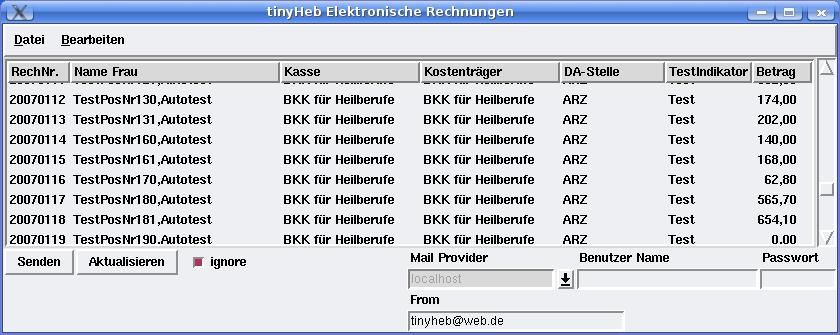
\includegraphics[width=80mm]{xauftrag}
\caption{Elektronische Rechnungen \label{kurz:xauftrag:fig}}
\end{figure}
Durch Anklicken einer Rechnungsnummer wird diese zum elektronischen Versand
ausgewählt. Über den Knopf \knopf{Senden} wird die Rechnung elektronisch
versand. Dabei wird die Rechnung sowohl an die entsprechende 
Datenannahmestelle geschickt, wie auch in Blindkopie an die Hebamme.
%
%
\section{Rechnungsbearbeitung}\label{kurz:rechnungsbearbeitung:kap}
Hat man eine oder mehrere Rechnungen erstellt, ist es notwendig, den
Zahlungseingang zu überwachen. Dazu dient die Maske 
\texttt{Rechnungsbearbeitung}. In diese Maske gelangt man aus dem
Hauptmenue über den Link \verb|versandte Rechnungen bearbeiten|.
Die Maske ist wie
auch die Maske Rechnungsgenerierung in zwei Teile gegliedert. Alle Rechnungen,
die bisher erstellt wurden, werden im oberen Teil der Maske angezeigt, dort
stehen zwei Knöpfe pro Rechnung zur Auswahl: 
% 
\begin{enumerate}[1.]
\item der Knopf \knopf{Bearbeiten}.
Über diesen Knopf werden die Daten der Rechnung
in den zweiten Teil der Maske übernommen. Dazu gehören insb. der Betrag
und der bisher gezahlte Betrag. Das Datum des
Rechnungseingangs und der gezahlte Betrag kann in den Feldern \feld{Zahldatum}
und \feld{Betrag gez.:} erfasst werden. Über den Knopf \knopf{Speichern}
werden die Daten gespeichert. Ist der bisher gezahlte Betrag und der aktuell
gezahlte Betrag kleiner als die ursprüngliche Rechnung, wird der Status auf
Teilzahlung gesetzt. Entspricht er der ursprünglichen Rechnung, bekommt diese
den Status erledigt.
\item der Knopf \knopf{Ansehen}.
Über diesen Knopf ist es möglich, sich
die original Rechnung anzusehen und bei Bedarf erneut zu drucken.
\end{enumerate}

Damit ist der komplette Zyklus einer Rechnung beschrieben. 
Details zur Erfassung von Stammdaten, Rechnungsposten, usw. 
finden sich in den nächsten Kapiteln.



%%% Local Variables: 
%%% mode: latex
%%% TeX-master: "anleitung"
%%% End: 


% $Id: anleitung.tex,v 1.19 2009/05/31 04:57:01 baum Exp $
% Tag $Name: tinyheb-1-6-3 $

% Copyright (C) 2004 - 2013 Thomas Baum <thomas.baum@arcor.de>
% Thomas Baum, 42719 Solingen, Germany

% This program is free software; you can redistribute it and/or modify
% it under the terms of the GNU General Public License as published by
% the Free Software Foundation; either version 2 of the License, or
% (at your option) any later version.

% This program is distributed in the hope that it will be useful,
% but WITHOUT ANY WARRANTY; without even the implied warranty of
% MERCHANTABILITY or FITNESS FOR A PARTICULAR PURPOSE.  See the
% GNU General Public License for more details.

% You should have received a copy of the GNU General Public License
% along with this program; if not, write to the Free Software
% Foundation, Inc., 59 Temple Place - Suite 330, Boston, MA 02111-1307, USA.


\chapter {Anleitung\label{anleitung}}
In diesem Kapitel ist die komplette Anleitung zu \tinyHeb\/ beschrieben. Zun�chst wird auf die Erfassung von Stammdaten eingegangen, inkl. einer �bersicht 
welche Plausibilit�ten Pr�fungen f�r die einzelnen Felder hinterlegt sind.
Im Abschnitt Rechnungserfassung werden die Besonderheiten bei der
Erfassung der Rechnung aufgezeigt. Es wird insbesondere beschrieben, welche
Rechnungsposten in welchen F�llen automatisch ermittelt werden. Es werden
aber auch die Grenzen des Programms gezeigt, d.h. an welchen Stellen muss
die Anwenderin selbst darauf achten, dass z.B. Zuschl�ge richtig erfasst
werden.

\section{Stammdatenerfassung\label{stammdatenerfassung:kap}}
\index{Stammdaten}
\index{Patientinnen|see{Stammdaten}}
In diesem Abschnitt werden alle Felder beschrieben, die erfasst werden
k�nnen und welche Auswirkung diese in der sp�teren Be-/ Verarbeitung haben.
Es wird gezeigt, wie ``Frauen'' angelegt, ge�ndert,
respektive gel�scht werden k�nnen und
welche Funktionen die einzelnen Kn�pfe auf der Maske haben.\par
�ber den Link \verb|Stammdaten| gelangt man aus dem Hauptmenue 
(Abbildung \vref{einstieg:fig}) in die Maske Stammdaten
(siehe Abbildung \vref{stammdatenerfassung:fig}).

\begin{figure}[ht]
\centering
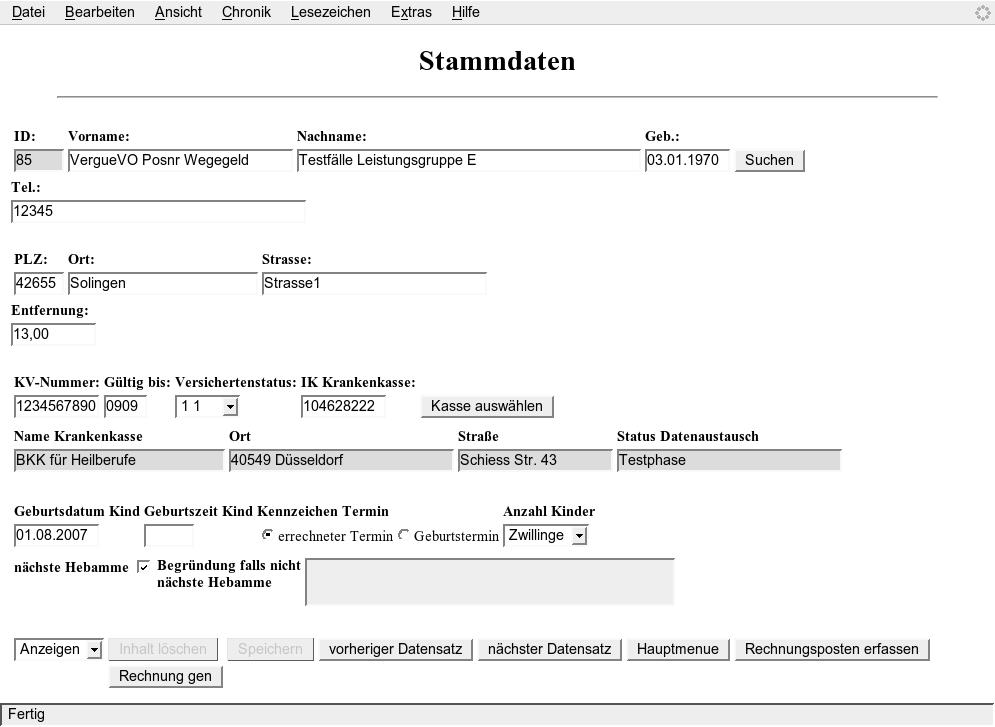
\includegraphics[width=9cm]{stammdaten}
\caption{Stammdatenerfassungsmaske\label{stammdatenerfassung:fig}}
\end{figure}

\subsection{Beschreibung der Stammdatenfelder}
Der Cursor steht nach Aufruf der Maske immer im ersten leeren  Feld.
Bei einer leeren Maske also im Feld \feld{Vorname}.
Folgende Felder sind auf der Maske vorhanden:
\begin{description}
\item[ID] Dieses Feld enth�lt die interne ID zum angezeigten Datensatz,
es wird automatisch gef�llt und kann nicht erfasst oder ge�ndert werden.
\item[Vorname] Dieses Feld enth�lt den Vornamen der Frau, es k�nnen maximal 30 Zeichen erfasst werden\footnote{im Rahmen des elektronischen Datenaustausches sind f�r den Vornamen nur 30 Zeichen vorgesehen}. Der Vorname wird in die sp�tere Rechnung �bernommen.
Eine Pr�fung ob der Vorname erfasst wird, existiert an dieser Stelle nicht.
\item[Nachname] Das Feld enth�lt den Nachnamen der Frau, es k�nnen maximal 47 Zeichen erfasst werden\footnote{im Rahmen des elektronischen Datenaustausches sind f�r den Nachnamen nur 47 Zeichen vorgesehen}. Der Nachname wird in die sp�tere Rechnung �bernommen.
Eine Pr�fung ob der Nachname erfasst wird, existiert an dieser Stelle nicht.
\item[Geb.] Dieses Feld enth�lt das Geburtsdatum der Frau. Das Datum wird
in die sp�tere Rechnng �bernommen. Die Erfassung muss
im Format TT.MM.JJJJ oder TT.MM.JJ erfolgen. 
Wird das Datum im Format TT.MM.JJ erfasst, erfolgt nach Verlassen des
Feldes automatisch die Ermittlung und Darstellung der 4-stelligen Jahreszahl.
Ein ung�ltiges Datum f�hrt zu der Fehlermeldung: Bitte g�ltiges Datum erfassen.
Das Speichern des Formulares mit ung�ltigen Werten ist nicht m�glich.
\item[Tel.] Das Feld enth�lt die Telefonnummer der Frau, es k�nnen beliebige
Zeichen erfasst werden. Das Feld hat rein informativen Charakter 
und wird in der weiteren Anwendung
nicht mehr verwendet\footnote{dies kann sich zuk�nftig �ndern, z.B. bei
Auswertungen oder Listen, die produziert werden, Stand 04.09.2005}.
\item[PLZ] Das Feld enth�lt die PLZ zur Anschrift der Frau. Es wird in die 
sp�tere Rechnung �bernommen. Es muss eine 5-stellige numerische Zahl
 erfasst werden. Das
bedeutet, eine 4-stellige PLZ, wie z.B. 04177 Leipzig,
muss mit f�hrender Null erfasst werden. Ob
die PLZ im Sinne der Post wirklich g�ltig ist oder nicht, wird nicht
gepr�ft. Ein nicht korrekter Wert f�hrt zu einer entsprechenden Fehlermeldung,
die durch Dr�cken des Knopfes \knopf{OK} best�tigt werden muss.
Das Speichern des Formulares mit ung�ltigen Werten ist nicht m�glich (siehe auch Feld Geb.).
Eine Pr�fung, ob die PLZ erfasst wird, existiert an dieser Stelle nicht.
\item[Ort] Das Feld enth�lt den Ort zur Anschrift der Frau, es k�nnen
maximal 25 Zeichen erfasst werden. Der Ort wird in die 
sp�tere Rechnung �bernommen. Eine Pr�fung, ob der Ort erfasst wird, exisiert
an dieser Stelle nicht.
\item[Strasse] Das Feld enth�lt die Strasse zur Anschrift der Frau, es k�nnen
maximal 30 Zeichen erfasst werden. Die Strasse wird in die 
sp�tere Rechnung �bernommen. Eine Pr�fung, ob die Strasse erfasst wird, 
exisiert an dieser Stelle nicht.
\item[Entfernung] Das Feld enth�lt die Entfernung von der Hebamme bis zur Frau.
Der Inhalt wird in die Maske Rechnungsposten erfassen �bernommmen.
\item[KV-Nummer] Das Feld enth�lt die Krankenversicherungsnummer der Frau, die
in die sp�tere Rechnung �bernommen wird.
Es muss 9 oder 10-stellig numerisch erfasst werden. 
Das bedeutet, es muss ggf. mit
f�hrenden Nullen erfasst werden. Ein nicht korrekter Wert f�hrt zu einer
entsprechenden Fehlermeldung, die durch Dr�cken des Knopfes \knopf{OK}
best�tigt werden muss (analog dem Feld PLZ). Eine Pr�fung, ob die KV-Nummer
erfasst wird, existiert an dieser Stelle nicht.
\item[G�ltig bis] Das Feld enth�lt die G�ltigkeitsdauer der Versichertenkarte
der Frau und wird in die sp�tere Rechnung �bernommen. Es muss im Format
MMJJ erfasst werden. Die Fehlerbehandlung erfolgt analog den Feldern
PLZ und KV-Nummer. Eine Pr�fung, ob das Feld erfasst wird, existiert an
dieser Stelle nicht,
\item[Versichertenstatus] 
\index{Versichertenstatus}
Das Feld enth�lt den Versichertenstatus der Frau
und wird in die sp�tere Rechnung �bernommen. Per Pop Down Menue k�nnen
die Werte '1 1', '3 1', 'privat', '1 9', '3 9','1 7','3 7','1 8','3 8','5 1',
'5 9','SOZ' ausgew�hlt werden.
\item[IK Krankenkasse] Das Feld enth�lt die IK Nummer der Krankenkasse der
Frau und wird in die sp�tere Rechnung �bernommen. Anhand der IK Nummer
wird der Name und die Rechnungsanschrift der Krankenkasse ermittelt. Ohne
die Angabe der IK Nummer kann keine ordnungsgem��e Rechnung produziert werden.
Die Nummer ist 9-stellig numerisch zu erfassen. Wird das Feld nur 7-stellig
numerisch erfasst, wird automatisch 10 vorangestellt, da in der Regel
die IK Nummer nur 7-stellig auf der Versichertenkarte angegeben ist.
Die Vorgehensweise bzgl.
der Fehlerkorrektur ist analog zu den Feldern \feld{PLZ} und \feld{Geb.}
\item[Name der Krankenkasse, Ort, Stra�e, Status Datenaustausch] 
Diese Felder enthalten die 
Anschrift der Krankenkasse sowie den Status zum Datenaustausch
und k�nnen nicht erfasst werden. Die Werte werden
anhand der IK Nummer der Krankenkasse automatisch nach dem Speichern
gef�llt. Wurde im Feld \feld{IK Krankenkasse} eine unbekannte IK Nummer
erfasst, erscheint im Feld \feld{Name der Krankenkasse} der Hinweistext:
``nicht bekannte IK angegeben''. Wurde im Feld \feld{Versichertenstatus} privat
ausgew�hlt, wird der Hinweistext: ``Privat versichert'' ausgegeben.
Im Feld \feld{Status Datenaustausch} ist angegeben in welchem Status mit dieser
Krankenkasse der Datenaustausch abgewickelt wird. M�gliche Werte sind:
\begin{enumerate}
\item 
kein elektronischer Datenaustausch
\item 
Testphase
\item
Erprobungsphase
\item
Echtbetrieb
\end{enumerate}
\item[Geburtsdatum Kind] Dieses Feld enth�lt das Geburtsdatum, bzw. den
errechneten Geburtstermin des Kindes und wird in die sp�tere Rechnung 
�bernommen. 
Anhand dieses Feldes werden u.a.
Materialpauschalen bei der Erfassung von Rechnungsposten ermittelt.
Die Plausipr�fungen erfolgen analog dem Feld \feld{Geb.} Eine Pr�fung,
ob das Geburtsdatum Kind erfasst wird, existiert nicht.
\item[Geburtszeit Kind]
In diesem Feld muss die Uhrzeit der Geburt erfasst werden. Es kann frei
gelassen werden, wenn es sich bei dem Geburtsdatum um den errechneten
Termin handelt oder die Uhrzeit nicht bekannt ist. 
Das Feld muss im Format HH:MM erfasst werden.
Ein nicht korrekter Wert f�hrt zu einer entsprechenden Fehlermeldung,
die durch Dr�cken des Knopfes \knopf{OK} best�tigt werden muss.
Das Speichern des Formulares mit ung�ltigen Werten ist nicht m�glich.
\footnote{Dieses Feld wird ab dem 01.02.2008 in die elektronische
Rechnung �bernommen.}
\item[Kennzeichen Termin]
�ber diesen Schalter wird gesteuert, ob es sich im Feld 
\feld{Geburtsdatum Kind}
um das Geburtsdatum,  bzw. den errechneten Geburtstermin des Kindes
handelt. Wird Geburtstermin angegeben, wird auf der Rechnung ``geboren am'' 
angedruckt, sonst wird ``ET'' angedruckt.
\footnote{Dieses Feld wird ab dem 01.02.2008 in die elektronische
Rechnung �bernommen.}
\item[Anzahl Kinder] Das Feld enth�lt die Anzahl der Kinder, die bei dem
Geburtsdatum angegebenen Termin zur Welt gebracht wurden. Sind mehrere
Kinder zur Welt gekommen, wird dies auf der sp�teren Rechnung ausgewiesen.
Per Pop Down Menue k�nnen bis zu vier Kinder ausgew�hlt werden.
\item[n�chste Hebamme] Dieses Feld enth�lt einen Schalter, ob die Hebamme,
die n�chste Hebamme ist. Das Feld hat rein informativen Charakter. Ist der
Schalter angekreuzt, ist das Feld \feld{Begr�ndung falls nicht n�chste
Hebamme} f�r die Erfassung gesperrt.
\item[Begr�ndung falls nicht n�chste Hebamme] Dieses Feld kann eine frei
formulierte Begr�ndung enthalten, falls die Hebamme nicht die n�chste Hebamme
ist. Das Feld hat rein informativen Charakter und wird in der weitere
Anwendung nicht verwendet. Eine Erfassung ist nur m�glich, wenn der Schalter
\feld{n�chste Hebamme} nicht gesetzt ist.
\end{description}
Erst bei der Rechnungserstellung wird gepr�ft, ob die Felder
\feld{Vorname, Nachname, Geburtsdatum Frau, Geburtsdatum Kind, KV-Nummer, Versichertenstatus, Geburtszeit Kind,
IK-Krankenkasse} gef�llt sind. Ist dies nicht der Fall, kann keine
Rechnung erstellt werden. Wobei die Felder \feld{KV-Nummer} und 
\feld{IK-Krankenkasse}
nur dann notwendig sind, wenn es sich um eine Kassenrechnung handelt.
Im Kapitel \vref{rechnungsgenerierung:kap} sind die Pr�fungen im Detail
beschrieben.

\subsection{Beschreibung der Kn�pfe im Stammdatenmenue}
\begin{description}
\item[Suchen] 
Mit dem Knopf \knopf{Suchen} kann eine weitere Maske ge�ffnet
werden, �ber die Frauen gesucht werden k�nnen. Die Beschreibung zu der
Suchmaske befindet sich in Abschnitt \vref{frauenauswahl:abs}.
In diese Maske werden die Werte aus den Feldern \feld{Vorname, Nachname}
sowie
\feld{Geb.} �bernommen und die Suche unmittelbar gestartet.
\item[Kasse ausw�hlen] 
Mit dem Knopf \knopf{Kasse ausw�hlen} wird ein Maske
ge�ffnet, �ber die Krankenkassen gesucht werden k�nnen. Die Beschreibung zu
der Suchmaske befindet sich in Abschnitt \vref{kassenauswahl:abs}. Eine
�bernahme von Daten, wie beim Knopf \knopf{Suchen} erfolgt nicht.
\item[Inhalt l�schen] 
Der Knopf \knopf{Inhalt l�schen} ist nur dann Aktiv, wenn in dem
Pop Down Menue vor dem Knopf der Wert Neu ausgew�hlt wurde. Wird der Knopf
gedr�ckt, werden die Feldinhalte aller Felder der Maske gel�scht und das
Pop Down Menue springt auf den Wert Anzeigen. Der Datensatz selbst wird
nicht gel�scht.
\item[Speichern/ L�schen] Der Knopf \knopf{Speichern} ist nur dann aktiv,
wenn im
Auswahlmenue entweder der Wert Neu oder �ndern gew�hlt wird. 
\par
Falls \knopf{Neu}
ausgew�hlt wurde, wird ein neuer Kundinnensatz in der Datenbank gespeichert
und das Pop Down Menue springt auf den Wert Anzeigen. Neben den oben
beschriebenen Plausibilit�ten Pr�fungen findet beim Speichern keine weitere
Pr�fung statt.\par
Falls \knopf{�ndern} gew�hlt wurde, wird der Datensatz, der sich in der Datenbank
befindet mit den angezeigten Werten �berschrieben und das Pop Down Menue
springt auf den Wert Anzeigen. Neben den oben beschriebenen
Plausibilit�tenpr�fungen finden keine weiteren Pr�fungen statt.

Falls im Pop Down Menue \knopf{L�schen} ausgew�hlt wurde, erh�lt der Knopf die
Beschriftung L�schen. Durch Dr�cken des Knopfes wird der Datensatz aus der
Datenbank gel�scht. Es wird bei der L�schung gepr�ft, ob schon Leistungen
erfasst wurden. Ist dies der Fall, kann der Datensatz nicht mehr gel�scht 
werden und es erscheint die Fehlermeldung ``L�schen nicht m�glich, es sind
schon Leistungen erfasst''. Wurde der Datensatz erfolgreich gel�scht, werden
alle Feldinhalte der Felder der Maske gel�scht und das Auswahlmenue
steht auf den Wert Anzeigen. Konnte der Datensatz nicht gel�scht werden,
bleiben die Inhalte der Felder erhalten. Das Auswahlmenue springt auf den 
Wert Anzeigen.
\item[vorheriger Datensatz] Dieser Knopf ist nur dann aktiv, wenn der Wert
des Pop Down Menues auf Anzeigen steht. Durch Dr�cken des Knopfes wird auf
den vorherigen Datensatz in der Datenbank gesprungen. Der vorherige Datensatz
ist derjenige, mit der n�chst kleineren ID, als die im Feld \feld{ID}
angezeigte. Ist
man am ersten Datensatz angekommen, bleibt dieser in der Maske erhalten.
\item[n�chster Datensatz] Dieser Knopf ist nur dann aktiv, wenn der Wert
des Pop Down Menues auf Anzeigen steht. Durch Dr�cken des Knopfes wird auf
den n�chsten Datensatz in der Datenbank gesprungen. Der n�chste Datensatz
ist derjenige, mit der n�chst h�heren ID, als die im Feld \feld{ID}
 aktuell angezeigte. Ist
man am letzten Datensatz angekommen, bleibt dieser in der Maske erhalten.
\item[Hauptmenue] �ber diesen Knopf gelangt man in das Hauptmenue.
Dabei ist zu beachten, dass nicht �berpr�ft wird, ob �nderungen oder Neu
erfasste Daten gespeichert wurden. Es wird sofort in die Maske Hauptmenue
gesprungen.
\item[Rechnungsposten erfassen] �ber diesen Knopf gelangt man in die Maske
zur Erfassung von Rechnungsposten. Ein Sprung in die Maske ist nur 
m�glich, wenn eine Kundin und \knopf{Anzeigen} ausgew�hlt ist. Die 
Stammdaten der Kundin werden in die Maske Rechnungsposten erfassen �bernommen.
\item[Rechnung gen] �ber diesen Knopf gelangt man in die Maske zum Ausdruck
der noch in Bearbeitung befindlichen Rechnungsposten. Ein Sprung in die Maske
ist nur dann m�glich, wenn eine Kundin und \knopf{Anzeigen} gew�hlt ist. Die
Stammdaten der Kundin werden in die Maske Rechnungsgenerierung �bernommen.
\end{description}

Sind alle Felder erfasst, m�ssen die Daten gespeichert werden. Dazu ist
es notwendig im Pop Down Menue unten links den Wert 'Neu' auszuw�hlen.
Sobald dies geschehen ist, wird der Knopf \knopf{Speichern} aktiv 
geschaltet. Dr�ckt man jetzt den Knopf \knopf{Speichern} werden die Daten
zu der Frau permanent abgelegt. Nach dem Speichern wird die Auswahl im 
Pop Down Menue unten links auf den Wert 'Anzeigen' gesetzt.




\section{Frauenauswahl}\label{frauenauswahl:abs}
In diesem Absatz ist beschrieben, wie Kundinnen im Datenbestand gesucht und
ausgew�hlt werden k�nnen.
In der Regel erfolgt der  Aufruf der Maske aus der 
Stammdatenerfassungsmaske (siehe
Seite \pageref{stammdatenerfassung:fig}) 
�ber den Knopf \knopf{Suchen}. Analoge Kn�pfe findet man in dem Masken der
Rechnungspostenerfassung (siehe Seite \pageref{rechnungspostenerfassen:fig})
und der
Rechnungsgenerierung (siehe Seite \pageref{rechnungsgenerierung:fig}).
Klickt man auf den Knopf \knopf{Suchen} wird ein neues Fenster mit der
�berschrift ``Frau suchen'' ge�ffnet\footnote{sollte das Fenster 
noch ge�ffnet sein, wird es in den 
Vordergrund des Bildschirms geholt.} 
(siehe Abbildung \vref{frauenauswahl:fig}). �ber die Felder \feld{Vorname,
Nachname, Geb. Frau, Geb. Kind, PLZ, Ort und Strasse} ist es m�glich die
Suchkriterien vorzugeben, d.h. es werden bei der Suche nur die Frauen
ausgegeben, bei denen alle vorgegebenen Werte vorhanden sind. Dabei ist
folgendes f�r die Felder zu beachten:

\begin{figure}[h]
\centering
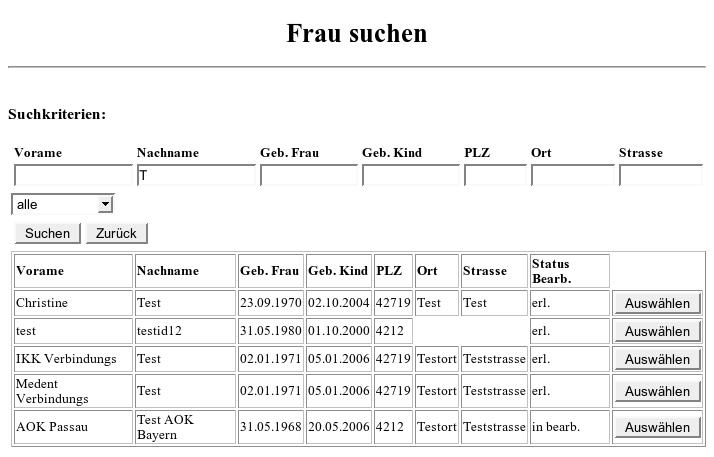
\includegraphics[width=9cm]{frauenauswahl}
\caption{Frauenauswahlmaske\label{frauenauswahl:fig}}
\end{figure}

\begin{description}
\item[Vorname] Es wird nur nach den Frauen gesucht, bei denen der Vorname 
einen Teil des Feldes enth�lt.
Wird z.B. im Feld \feld{Vorname} ``Maria'' erfasst,
w�rde Maria Luise und Anna Maria ermittelt werden.
\item[Nachname] Es wird nur nach den Frauen gesucht, bei denen der Nachname mit
dem Feldinhalt beginnt. Wird z.B. im Feld \feld{Nachname} ``D'' erfasst,
w�rden alle Frauen deren Nachname mit ``D'' beginnt ermittelt werden.
\item[Geb. Frau] Es wird nur nach den Frauen gesucht, die an diesem Tag geboren
sind. Das Feld ist im Format TT.MM.JJJJ zu erfassen, die Plausipr�fungen sind
analog der Pr�fungen, die im Kapitel Stammdatenerfassung 
(Seite \pageref{stammdatenerfassung:kap}) beschrieben sind.
\item[Geb. Kind] Es wird nur nach den Frauen gesucht, deren Kinder
an diesem Tag geboren wurden.
Das Feld ist im Format TT.MM.JJJJ zu erfassen, die Plausipr�fungen sind
analog der Pr�fungen, die im Kapitel Stammdatenerfassung 
(Seite \pageref{stammdatenerfassung:kap}) beschrieben sind.
\item[PLZ] Es wird nur nach den Frauen gesucht, deren Adresse die im Feld
\feld{PLZ} erfasste PLZ exakt enth�lt. Die Plausipr�fungen sind analog
der Pr�fungen, die im Kapitel Stammdatenerfassung (Seite 
\pageref{stammdatenerfassung:kap}) beschrieben sind.
\item[Ort] Es wird nur nach den Frauen gesucht, bei denen der Ort einen
Teil des Feldes enth�lt. Wird z.B. im Feld \feld{Ort} ``ing'' erfasst,
w�rden Frauen an den Orten Sol\textbf{ing}en und Emmend\textbf{ing}en ermittelt.
\item[Strasse] Es wird nur nach den Frauen gesucht, bei denen die Stra�e einen
Teil des Feldes enth�lt. Wird z.B. im Feld \feld{Strasse} ``el'' erfasst,
w�rden alle Frauen die in den Stra�en D\textbf{el}ler Str. und 
Ohligser F\textbf{el}d ermittelt.
\end{description}

�ber das Auswahlfeld �ber
dem Knopf \knopf{Suchen} l�sst sich die Suche zus�tzlich einschr�nken auf alle
Frauen bei denen Positionen existieren, die in einem Status ungleich
erledigt sind.
Ist der Aufruf der Maske aus der Stammdatenerfassung
erfolgt, werden die Werte Vorname, Nachname sowie das Geburtsdatum der Frau
in die Suchkriterien �bernommen und die Suche wird unmittelbar gestartet.
Die Felder k�nnen jederzeit mit neuen Suchkriterien gef�llt und die Suche
�ber den Knopf \knopf{Suchen} gestartet werden.

Das Ergebnis der Suche wird unmittelbar unter den Suchkriterien ausgegeben.
Neben den Daten zu Name und Anschrift wird auch der Bearbeitungsstatus
angezeigt, folgende Status sind m�glich:
\begin{description}
\item[in bearb.] 
Es sind keine oder Rechnungsposten erfasst, f�r die noch
keine Rechnung erstellt wurde.
\item[Rechnung] 
Es wurde eine Papierrechnung erstellt. Es sind keine weiteren
Rechnungsposten vorhanden, f�r die noch eine Rechnung erstellt werden muss.
\item[Edi Rech.] 
Es wurde eine elektronische Rechnung erstellt. Es sind
keine weiteren Rechnungsposten vorhanden, f�r die noch eine Rechnung
erstellt werden muss.
\item[Teilzahl.] 
Es wurde f�r eine Rechnung eine Teilzahlung geleistet. Es
ist weder eine weitere Rechnung vorhanden, f�r die noch keine Zahlung erfolgt
ist, noch sind weitere Rechnungsposten vorhanden, f�r die noch eine Rechnung erstellt werden muss.
\item[Mahnung] 
Es wurde f�r eine Rechnung bereits eine Mahnung erstellt, 
dabei wird angegeben, wie viele Mahnung bisher erstellt wurden.
\item[erl.] 
Es sind weder offene Rechnungsposten noch Rechnungen vorhanden.
\end{description}

�ber den Knopf \knopf{Ausw�hlen} werden die Daten der Frau in die Maske
�bernommen, aus der die Suchfunktion aufgerufen wurde. Die Maske ``Frau Suchen''
wird danach geschlossen.

Falls keine Frau den gew�nschten Suchkriterien entspricht, kann entweder
durch Klicken des Knopfes \knopf{Zur�ck} die Maske ``Frau Suchen''
geschlossen werden, oder es k�nnen andere Suchkriterien erfasst werden.





\section{Krankenkassen\label{krankenkassenerfassung:kap}}
\index{Krankenkassen}
In diesem Abschnitt werden alle Felder beschrieben, die erfasst werden
k�nnen und welche Auswirkung diese in der sp�teren Be-/ Verarbeitung haben.
Es wird gezeigt, wie �ber die Maske ``Krankenkassen'' angelegt, ge�ndert,
respektive gel�scht werden k�nnen und
welche Funktionen die einzelnen Kn�pfe in der Maske haben. In der Regel
sollte die manuelle Erfassung von Krankenkassen nicht notwendig sein,
da die aktuellen Daten der Krankenkassen in den so genannten 
Kostentr�gerdateien enthalten sind, die sich mit \tinyHeb\/ automatisch
verarbeiten lassen. Wie dies Funktioniert, ist im Anhang in Kapitel
\vref{anhang:ktrdat} beschrieben.

�ber den Link \verb|Krankenkassen| gelangt man aus dem Hauptmenue 
(Abbildung \vref{einstieg:fig}) in die Maske Krankenkassen
(siehe Abbildung \vref{krankenkassenerfassung:fig}).
\begin{figure}[ht]
\centering
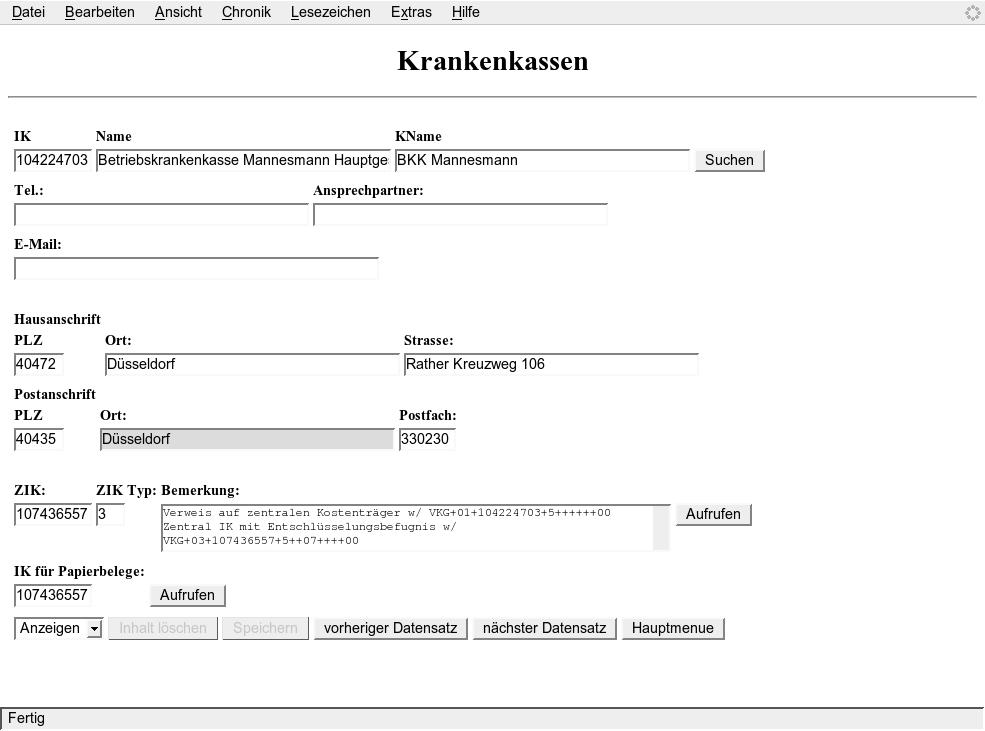
\includegraphics[width=9cm]{krankenkassen}
\caption{Krankenkassenerfassungsmaske\label{krankenkassenerfassung:fig}}
\end{figure}
\subsection{Beschreibung der Krankenkassenfelder}
Der Cursor steht nach Aufruf der Maske im Feld \feld{Name}, bzw. im ersten
leeren Feld nach der IK Nummer.
Folgende Felder sind auf der Maske vorhanden:
\begin{description}
\item[IK] 
Dieses Feld enth�lt die IK Nummer der Krankenkasse.
\item[Name]
Dieses Feld enth�lt den Namen der Krankenkasse. Hat die Krankenkasse einen
sehr langen Namen, ist nur der erste Teil des Names sichtbar.
Eine Pr�fung ob der Nname erfasst wird, existiert an dieser Stelle nicht.
\item[KName] 
Das Feld enth�lt den Kurznamen der Krankenkasse. Dieser Name wird sp�ter
in der Rechnung angedruckt.
Eine Pr�fung ob der Kurzname erfasst wird, existiert an dieser Stelle nicht.
\item[Tel.] 
Das Feld enth�lt die Telefonnummer der Krankenkasse, 
es k�nnen beliebige
Zeichen erfasst werden. Das Feld hat rein informativen Charakter 
und wird in der weiteren Anwendung
nicht mehr verwendet.
\item[E-Mail]
Das Feld enth�lt die E-Mail Adresse der Krankenkasse und ist i.d.R. nur 
f�r Datenannahmestellen gef�llt.
\end{description}

\paragraph{Hausanschrift}
\begin{description}
\item[PLZ] 
Das Feld enth�lt die PLZ zur Anschrift der Krankenkasse. 
Es wird in die 
sp�tere Rechnung �bernommen. Es muss eine 5-stellige numerische Zahl
 erfasst werden. Das
bedeutet, eine 4-stellige PLZ, wie z.B. 04177 Leipzig,
muss mit f�hrender Null erfasst werden. Ob
die PLZ im Sinne der Post wirklich g�ltig ist oder nicht, wird nicht
gepr�ft. Ein nicht korrekter Wert f�hrt zu einer entsprechenden Fehlermeldung,
die durch Dr�cken des Knopfes \knopf{OK} best�tigt werden muss.
Das Speichern des Formulares mit ung�ltigen Werten ist nicht m�glich.
Eine Pr�fung, ob die PLZ erfasst wird, existiert an dieser Stelle nicht.
\item[Ort] 
Das Feld enth�lt den Ort zur Anschrift der Krankenkasse. Der Ort wird in die 
sp�tere Rechnung �bernommen. Eine Pr�fung, ob der Ort erfasst wird, exisiert
an dieser Stelle nicht.
\item[Strasse] 
Das Feld enth�lt die Strasse zur Anschrift der Krankenkasse, Die Strasse 
wird in die 
sp�tere Rechnung �bernommen. Eine Pr�fung, ob die Strasse erfasst wird, 
exisiert an dieser Stelle nicht.
\end{description}

\paragraph{Postanschrift}
Besitzt die Krankenkasse ein Postfach, sind die Felder unter der
�berschrift Postanschrift gef�llt. Da der Ort identisch ist, wird dieser aus
der Hausanschrift �bernommen. Falls eine Postanschrift vorhanden ist,
wird die sp�tere Rechnung an die Postanschrift und nicht die Hausanschrift
verschickt.
\begin{description}
\item[PLZ] 
Das Feld enth�lt die PLZ zur Anschrift der Krankenkasse. 
Es wird in die 
sp�tere Rechnung �bernommen. Es muss eine 5-stellige numerische Zahl
 erfasst werden. Das
bedeutet, eine 4-stellige PLZ, wie z.B. 04177 Leipzig,
muss mit f�hrender Null erfasst werden. Ob
die PLZ im Sinne der Post wirklich g�ltig ist oder nicht, wird nicht
gepr�ft. Ein nicht korrekter Wert f�hrt zu einer entsprechenden Fehlermeldung,
die durch Dr�cken des Knopfes \knopf{OK} best�tigt werden muss.
Das Speichern des Formulares mit ung�ltigen Werten ist nicht m�glich.
Eine Pr�fung, ob die PLZ erfasst wird, existiert an dieser Stelle nicht.
\item[Ort] 
Das Feld ist nich erfassbar und wird aus dem Feld \feld{Ort} der
Hausanschrift �bernommen.
\item[Postfach] 
Das Feld enth�lt Nummer des Postfaches zur Anschrift der Krankenkasse.
Das Postfach wird in die 
sp�tere Rechnung �bernommen. Eine Pr�fung, ob ein Postfach erfasst wird, 
exisiert an dieser Stelle nicht.
\end{description}

\paragraph{}

\begin{description}
\item[ZIK]
\index{ZIK}
In diesem Feld ist eine IK Nummer angegeben, mit der die Krankenkasse
verkn�pft ist. Dies kann z.B. ein Kostentr�ger oder einer Datenannahmestelle
sein.
\item[ZIK Typ]
\index{ZIK Typ}
In diesem Feld ist die Art der Verkn�pfung zwischen Krankenkasse und der
``zentral IK'' angegeben. In \tinyHeb\/ existieren vier verschiedene Arten
von Verkn�pfungen:

\begin{enumerate}
\item[0] 
Es existiert keine Verkn�pfung.
\item[1]
Bei der im Feld \feld{ZIK} angegebenen IK Nummer handelt es sich um den
Kostentr�ger zur angezeigten Krankenkasse.
\item[2]
Bei der im Feld \feld{ZIK} angegebenen IK Nummer handelt es sich um eine
Datenannahmestelle ohne Entschl�sselungsbefugnis. Die angezeigte Krankenkasse
ist Datenannahmestelle mit Entschl�sselungsbefugnis. Die elektronische
Rechnung muss an die IK im \feld{ZIK} geschickt werden. Dabei handelt es
sich um den so genannten physikalischen Empf�nger der Daten \cite{ktrdat}.
\item[3]
Bei der im Feld \feld{ZIK} angegebenen IK Nummer handelt es sich um eine
Datenannahmestelle mit Entschl�sselungsbefugnis.
\end{enumerate}

\item[Bemerkung]
In diesem Feld k�nnen beliebige Informationen zu Krankenkasse hinterlegt
werden. Im Rahmen des automatischen Einlesens der Kostentr�gerdateien wird
dieses Feld �berschrieben. Angzeigt werden Informationen aus den 
Kostentr�gerdateien, die zur Ermittlung der Felder 
\feld{ZIK}, \feld{ZIK Typ} und \feld{IK f�r Papierbelege} genutzt wurden.
\item[IK f�r Papierbelege]
In diesem Feld ist die IK Nummer angegeben, an die die Papierbelege, bzw.
Urbelege geschickt werden m�ssen. Dieses Feld wird nur genutzt, wenn der
Parameter Belege auf 1 steht, siehe \vref{programmsteuerung_parm}.
\end{description}


\subsection{Beschreibung der Kn�pfe im Krankenkassenmenue}
\begin{description}
\item[Suchen] 
Mit dem Knopf \knopf{Suchen} kann eine weitere Maske ge�ffnet
werden, �ber die Krankenkassen gesucht werden k�nnen. Die Beschreibung zu der
Suchmaske befindet sich in Abschnitt \vref{kassenauswahl:abs}.
\item[Aufrufen] 
Der Knopf \knopf{Aufrufen} hinter dem Feld
\feld{Bemerkung} wird nur angezeigt, wenn das Feld \feld{ZIK} gef�llt ist. 
Die im Feld \feld{ZIK} angezeigte IK Nummer wird in der Maske
Krankenkassen aufgerufen.
\item[Aufrufen] 
Der Knopf \knopf{Aufrufen} hinter dem Feld
\feld{IK f�r Papierbelege} wird nur angezeigt, 
wenn das Feld \feld{IK f�r Papierbelege} gef�llt ist. 
Die im Feld \feld{IK f�r Papierbelege} angezeigte IK Nummer wird in der Maske
Krankenkassen aufgerufen.
\item[Inhalt l�schen] 
Der Knopf \knopf{Inhalt l�schen} ist nur dann
Aktiv, wenn in dem
Pop Down Menue vor dem Knopf der Wert Neu ausgew�hlt wurde. Wird der Knopf
gedr�ckt, werden die Feldinhalte aller Felder der Maske gel�scht und das
Pop Down Menue springt auf den Wert Anzeigen. Der Datensatz selbst wird
nicht gel�scht.
\item[Speichern/ L�schen] Der Knopf \knopf{Speichern} ist nur dann aktiv,
wenn im
Auswahlmenue entweder der Wert Neu oder �ndern gew�hlt wird. 
\par
Falls \knopf{Neu}
ausgew�hlt wurde, wird eine neue Krankenkasse in der Datenbank gespeichert
und das Pop Down Menue springt auf den Wert Anzeigen. Neben den oben
beschriebenen Plausibilit�ten Pr�fungen findet beim Speichern keine weitere
Pr�fung statt.\par
Falls \knopf{�ndern} gew�hlt wurde, wird der Datensatz, der sich in der Datenbank
befindet mit den angezeigten Werten �berschrieben und das Pop Down Menue
springt auf den Wert Anzeigen. Neben den oben beschriebenen
Plausibilit�tenpr�fungen finden keine weiteren Pr�fungen statt.

Falls im Pop Down Menue \knopf{L�schen} ausgew�hlt wurde, erh�lt der Knopf die
Beschriftung L�schen. Durch Dr�cken des Knopfes wird die Krankenkasse aus der
Datenbank gel�scht. Alle Feldinhalte der Felder der Maske werdem gel�scht 
und das Auswahlmenue
steht auf den Wert Anzeigen. 
\item[vorheriger Datensatz] 
Dieser Knopf ist nur dann aktiv, wenn der Wert
des Pop Down Menues auf Anzeigen steht. Durch Dr�cken des Knopfes wird auf
den vorherigen Datensatz in der Datenbank gesprungen. Der vorherige Datensatz
ist derjenige, mit der n�chst kleineren IK Nummer, als die im Feld 
\feld{IK} angezeigte. Ist
man am ersten Datensatz angekommen, bleibt dieser in der Maske erhalten.
\item[n�chster Datensatz] 
Dieser Knopf ist nur dann aktiv, wenn der Wert
des Pop Down Menues auf Anzeigen steht. Durch Dr�cken des Knopfes wird auf
den n�chsten Datensatz in der Datenbank gesprungen. Der n�chste Datensatz
ist derjenige, mit der n�chst h�heren IK Nummer, als die im Feld 
\feld{IK} aktuell angezeigte. Ist
man am letzten Datensatz angekommen, bleibt dieser in der Maske erhalten.
\item[Hauptmenue] 
�ber diesen Knopf gelangt man in die Maske Hauptmenue.
Dabei ist zu beachten, dass nicht �berpr�ft wird, ob �nderungen oder Neu
erfasste Daten gespeichert wurden. Es wird sofort in die Maske Hauptmenue
gesprungen.
\end{description}

Sind alle Felder erfasst, k�nnen die Daten gespeichert werden. Dazu ist
es notwendig im Pop Down Menue unten links den Wert 'Neu' auszuw�hlen.
Sobald dies geschehen ist, wird der Knopf \knopf{Speichern} aktiv 
geschaltet. Dr�ckt man jetzt den Knopf \knopf{Speichern} werden die Daten
zur Krankenkasse permanent abgelegt. Nach dem Speichern wird die Auswahl im 
Pop Down Menue unten links auf den Wert 'Anzeigen' gesetzt.




\section{Kassenauswahl}\label{kassenauswahl:abs}
In diesem Absatz ist beschrieben, wie Krankenkassen im Datenbestand gesucht und
ausgew�hlt werden k�nnen.
In der Regel erfolgt der  Aufruf der Maske aus der 
Krankenkassenerfassungsmaske (siehe
Seite \pageref{krankenkassenerfassung:fig}) 
�ber den Knopf \knopf{Suchen}. Einen analogen Knopf findet man in der Maske 
Stammdatenerfassung (siehe Seite \pageref{stammdatenerfassung:fig}).
Klickt man auf den Knopf \knopf{Suchen} wird ein neues Fenster mit der
�berschrift ``Krankenkasse suchen'' ge�ffnet\footnote{sollte das Fenster noch ge�ffnet sein, wird es in den Vordergrund des Bildschirms geholt.}

(Abbildung \vref{kassenauswahl:fig}). �ber die Felder \feld{IK,
Name, KName, Ort, PLZ Hausanschrift, PLZ Postfach} ist es m�glich die
Suchkriterien vorzugeben, d.h. es werden bei der Suche nur die Krankenkassen
ausgegeben, bei denen alle vorgegebenen Werte vorhanden sind. Dabei ist
folgendes f�r die Felder zu beachten:

\begin{figure}[h]
\centering
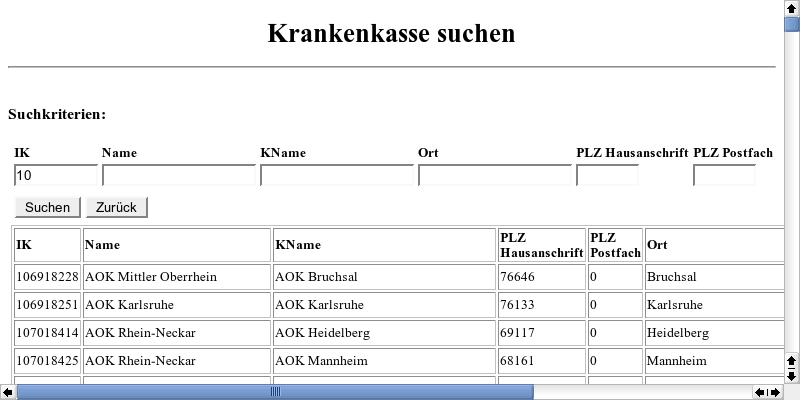
\includegraphics[width=9cm]{kassenauswahl}
\caption{Kassenauswahlmaske\label{kassenauswahl:fig}}
\end{figure}

\begin{description}
\item[IK] Es wird nur nach den Krankenkassen gesucht, bei denen die IK Nummer 
einen Teil des Feldes enth�lt.
Wird z.B. im Feld \feld{IK} ``70184'' erfasst,
w�rde IK 107018414, 107018425 und 107018436 ermittelt werden.
\item[Name] Es wird nur nach den Krankenkassen gesucht, bei denen der
Name einen Teil des Feldes enth�lt
Wird z.B. im Feld \feld{Name} ``Solingen'' erfasst,
w�rden alle Krankenkassen deren Name ``Solingen'' enth�lt ermittelt werden.
Wird z.B. im Feld \feld{Name} ``Solingen'' erfasst, w�rde
``AOK Solingen'', ``Betriebskrankenkasse Mannesmann Gesch�ftsstelle Solingen''
und ``IKK Nordrhein RD Solingen'' ermittelt werden.
\item[KName]
Es wird nur nach den Krankenkassen gesucht, bei denen der
Name einen Teil des Feldes enth�lt
Wird z.B. im Feld \feld{KName} ``IKK Nordrhein'' erfasst,
werden alle Krankenkassen ermittelt, deren Name ``IKK Nordrhein'' enth�lt.
\item[Ort] 
Es wird nur nach den Krankenkassen gesucht, bei denen der Ort einen Teil
des Feldes enth�lt.
Wird z.B. im Feld \feld{Ort} ``F�rth'' erfasst, werden
die Krankenkassen in ``F�rth'' und ``Wipperf�rth'' ermittelt.
\item[PLZ Hausanschrift] 
Es wird nur nach den Krankenkassen gesucht, bei denen die Postleitzahl der
Hausanschrift mit denen im Feld angegebenen Werten beginnt.
Wird z.B. im Feld \feld{PLZ Hausanschrift} ``4271'' erfasst, werden die
Krankenkassen ``Betriebskrankenkasse Bergisch Land Die Bergische Krankenkasse'' und ``Betriebskrankenkasse Krups/Zwilling'' ermittelt.
\item[PLZ Postfach] 
Es wird nur nach den Krankenkassen gesucht, bei denen die Postleitzahl des
Postfaches mit denen im Feld angegebenen Werten beginnt.
Wird z.B. im Feld \feld{PLZ Hausanschrift} ``427'' erfasst, werden die
Krankenkassen ``Betriebskrankenkasse Bergisch Land Die Bergische Krankenkasse'', ``Betriebskrankenkasse Krups/Zwilling'' und 
``IKK Nordrhein RD f�r den Kreis Mettmann'' ermittelt.
\end{description}
Die Suche Startet, nachdem der Knopf \knopf{Suchen} gedr�ckt wird.
Das Ergebnis der Suche wird unmittelbar unter den Suchkriterien ausgegeben.

�ber den Knopf \knopf{Ausw�hlen} werden die Daten der Krankenkasse in die Maske
�bernommen, aus der die Suchfunktion aufgerufen wurde. 
Die Maske ``Krankenkasse suchen''
wird danach geschlossen.

Falls keine Krankenkasse den gew�nschten Suchkriterien entspricht, 
kann entweder durch Klicken des Knopfes \knopf{Zur�ck} die 
Maske ``Krankenkasse suchen''
geschlossen, oder es k�nnen andere Suchkriterien erfasst werden.



\section{Erfassen von Rechnungsposten\label{rechnungspostenerfassung:kap}}
\index{Rechnungsposten}
In diesem Abschnitt werden die M�glichkeiten der Rechnungspostenerfassung
aufgezeigt. Es wird beschrieben, welche Positionsnummern automatisch
angew�hlt werden, welche Plausibilit�tenpr�fungen existieren, 
aber auch wo die Grenzen von \tinyHeb\/ sind. Es
ist insbesondere zu beachten, dass \tinyHeb\/ der Hebamme nicht das
Denken abnimmt ;-), sondern eine Hilfe f�r die Abrechnung gegen�ber den
Krankenkassen, bzw. den privaten Kundinnen darstellt.

Es gibt verschiedene Wege um in die Rechnungsposten Erfassung zu gelangen.
Aus dem Hauptmenue (Abbildung \vref{einstieg:fig})
gelangt man �ber den Link \verb|Rechnungsposten erfassen|
in die Maske zur Rechnungspostenerfassung (Abbildung 
\vref{rechnungspostenerfassen:fig}). Aus der Maske Rechnungsgenerierung
�ber den Knopf \knopf{Rechnungsposten erfassen} und aus der Maske Stammdaten
�ber den Knopf \knopf{Rechnungsposten erfassen}. Erfolgt der Aufruf
aus den Masken Rechnungsgenerierung oder Stammdaten, werden die Daten
der aktuell in der Anzeige befindlichen Frau in die Maske Rechnungsposten
erfassen �bernommen. 

\begin{figure}[ht]
\centering
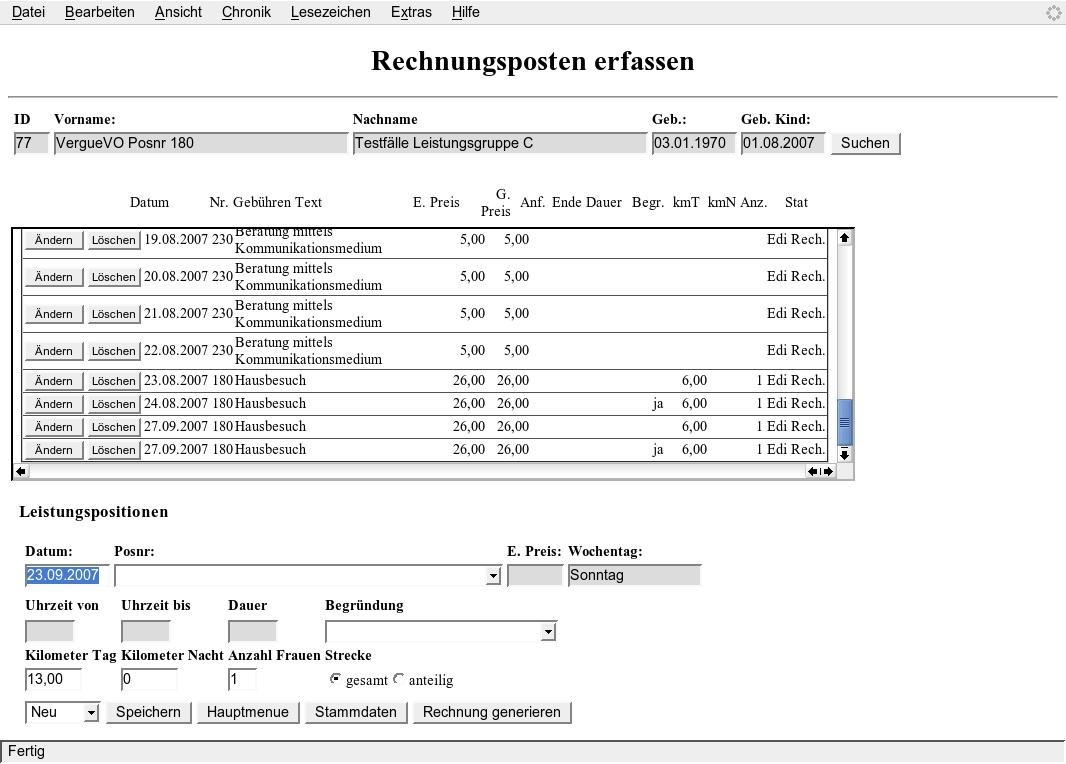
\includegraphics[width=9cm]{rechnungspostenerfassen}
\caption{Rechnungsposten erfassen\label{rechnungspostenerfassen:fig}}
\end{figure}

Wie schon in der Kurzanleitung beschrieben, ist
die Maske in drei Teile gegliedert. Im oberen Teil werden Daten zur Frau
angezeigt, die aktuell bearbeitet wird. In der Mitte werden die bisher
erfassten Rechnungsposten angzeigt. Im unteren Teil findet die Erfassung
der einzelnen Rechnungsposten statt.

\paragraph{Daten zur Frau}
Im oberen Bereich werden die wesentlichen Daten zur Frau angezeigt. Dazu
geh�ren, die ID, Vor- und Nachname, sowie das Geburtsdatum der Frau und
des Kindes. Diese Felder k�nnen nicht erfasst werden. Soll eine andere
Frau ausgew�hlt werden, muss dies �ber den Knopf \knopf{Suchen} geschehen.
Die Beschreibung zur Suchmaske befindet sich im Abschnitt 
\vref{frauenauswahl:abs}. Es werden keine Informationen in die Suchmaske
�bernommen.

\paragraph{bisher erfasste Rechnungsposten}
Im mittleren Abschnitt werden die bisher erfassten Posten angezeigt.
Es werden die Felder Datum (Datum der Leistungserbringung), die 
Positionsnummer, die Kurzbezeichnung der Positionsnummer, der Preis
der einzelnen Positionsnummer, der Gesamtpreis, ggf. Anfang und Ende
sowie die Dauer des Leistungszeitraumes, ob eine Begr�ndung erfasst wurde,
die Kilometeranzahl Tag (kmT) und Nacht (kmN), wie viele Frauen besucht
wurden und der Status der Rechnungsposition gezeigt.

Der Gesamtpreis ist in der Regel identisch mit dem Einzelpreis. Bei
Positionsnummern, die nach Dauer berechnet werden, wie z.B.
``Hilfe bei Beschwerden'', wird je nach Dauer und Positionsnummer die Dauer
mit dem Einzelpreis multipliziert und angezeigt.
Genau in diesen F�llen wird angezeigt, wann mit der Leistung begonnen, bzw.
wann sie beendet wurde. 

Ist bei einem Rechnungsposten nur die Anfangszeit erfasst worden\footnote{dies
ist sinnvoll, damit die entsprechenden
Positionsnummern f�r Nacht, Sonn- und Feiertagszuschlag automatisch ermittelt 
werden k�nnen}, z.B.
bei Positionsnummer 180 ``Hausbesuch nach der Geburt'' wird nur die 
Anfangszeit angezeigt, Ende und Dauer bleiben leer.
In allen anderen F�llen bleiben die Felder f�r
Anfang, Ende und Dauer leer. 
Bei Anzeige des Einzel- und Gesamtpreises wird die HebGV zu Grunde gelegt.
Falls es sich um eine Privatpatientin\index{Privatpatientin}
 handelt, werden die einzelnen
Rechnungsposten mit dem korrekten Preis erst in der Maske 
Rechnungsgenerierung angezeigt.

Ist eine Begr�ndung bei der einzelnen Position erfasst worden, wird unter
Begr. ``ja'' angezeigt, auch dieses Feld wird nur angezeigt, wenn eine
Begr�ndung erfasst wurde.

Analoges gilt f�r die Felder kmT und kmN, sowie Anzahl. Diese Felder werden
nur angezeigt, wenn Kilometer erfasst wurden.

Ganz Rechts wird der Status der einzelnen Position angezeigt, folgende
Status sind m�glich.
\begin{description}
\item[in bearb.] 
F�r diesen Posten wurde noch keine Rechnung erstellt.
\item[Rechnung] 
F�r diesen Posten wurde eine Papierrechnung erstellt. 
\item[Edi Rech.] 
F�r diesen Posten wurde eine elektronische Rechnung erstellt. 
\item[Mahnung]
F�r diesen Posten wurde bereits eine Mahnung erstellt, dabei wird angegeben, 
wie viele Mahnung bisher erstellt wurden.
\item[erl.] 
Dieser Rechnungsposten wurde schon beglichen.
\end{description}

Ist der Status ungleich ``in bearb.'', ist eine �nderung oder L�schung
dieses Postens nicht mehr m�glich.
�ber den Knopf \knopf{�ndern} werden die Informationen der entsprechenden
Position in den unteren Bereich der Maske �bernommen und die Daten k�nnen
ge�ndert werden.
�ber den Knopf \knopf{L�schen} wird die entsprechende Position sofort
gel�scht. Gibt es von dieser Position abh�ngige Positionsnummern, werden
diese ebenfalls gel�scht. D.h. wenn z.B. ein Rechnungsposten f�r 
Positionsnummer 190 ``Zuschlag 1. Besuch nach der Geburt'' gel�scht wird,
wird die entsprechende Materialpauschale ebenfalls gel�scht. Aber bitte
keine Sorgen machen, \tinyHeb\/ ermittelt automatisch, ob f�r einen
anderen Tag der ``Zuschlag 1. Besuch nach der Geburt'' berechnet werden
muss und wird dann auch die entsprechende Materialpauschale automatisch
ausw�hlen.

\subsection{Erfassung der Rechnungspositionen}
In diesem Abschnitt werden zun�chst die einzelnen Felder und Kn�pfe
beschrieben. Danach schlie�t sich eine Beschreibung f�r jede
Positionsnummer aus der Hebammen-Verg�tungs\-ver\-ordnung, bzw. HebGV an, 
mit einer Beschreibung, welche
Plausibilit�tenpr�fungen f�r die jeweilige Positionsnummer existieren,
respektive, welche weiteren Positionsnummern automatisch angew�hlt werden.

\subsection{Felder und Kn�pfe}
Folgende Felder sind in der Maske vorhanden:

\begin{description}
\item[Datum] 
Datum der Leistungserbringung. In diesem Feld ist zu erfassen, wann
die Leistung erbracht wurde, bzw. an welchem Tag eine Auslage entstanden ist.
D.h. wann z.B. eine Salbe verabreicht wurde.
Die Erfassung muss im Format TT.MM.JJJJ oder TT.MM.JJ erfolgen. 
Wird das Datum im Format TT.MM.JJ erfasst, erfolgt nach Verlassen des
Feldes automatisch die Ermittlung und Darstellung der 4-stelligen Jahreszahl.
Ein ung�ltiges Datum f�hrt zu der Fehlermeldung: Bitte g�ltiges Datum erfassen.
Das Speichern des Formulares mit ung�ltigen Werten ist nicht m�glich.
\item[Posnr]
�ber dieses Pop-Down-Feld kann die entsprechende Positionsnummer zu der
erbrachten Leistung ausgew�hlt werden, bzw. die interne Positionsnummer
f�r die entsprechende Materialien.
\item[Anzahl Kurse]
Dieses Feld wird nur dann auf der Maske dargestellt, wenn Positionsnummer 7,
070, 40 oder Positionsnummer 270 ausgew�hlt wird. 
In diesen F�llen l�sst sich erfassen,
wie viele Kurse durchgef�hrt wurden. Die jeweiligen einzelnen
Rechnungsposten werden automatisch generiert. Dazu werden die Werte aus
den Feldern \feld{Uhrzeit von} und \feld{Uhrzeit bis} �bernommen, 
der Inhalt des Feldes \feld{Datum} wird jeweils um sieben Tage erh�ht.
\item[E. Preis] 
Dieses Feld enth�lt den Einzelpreis zu der im Feld \feld{Posnr} ausgew�hlten
Positionsnummer, es wird angezeigt, sobald das Feld Positionsnummer
verlassen wurde. Das Feld ist nicht erfassbar. Es wird immer der
Preis gem�� HebGV angezeigt. Falls es sich um eine Privatkundin handelt,
wird erst in der Maske Rechnungsgenerierung der korrekte Preis angezeigt.
\item[Wochentag]
Dieses Feld enth�lt den Wochentag zu dem im Feld \feld{Datum} erfassten Datum.
Es wird aktualisiert, sobald das Feld \feld{Datum} verlassen wird.
Das Feld ist nicht erfassbar.
\item[Uhrzeit von]
Dieses Feld enth�lt die Uhrzeit ab der mit der Leistungserbringung begonnen
wurde. Es ist f�r alle Positionsnummern erfassbar. Zwingend ist es zu erfassen,
wenn es sich um eine Positionsnummer handelt,
bei der eine Zeitangabe notwendig ist, das ist z.B. bei Positionsnummer 050
``Hilfe bei Beschwerden'' der Fall. Bei allen Positionsummern f�r die ein
Zuschlag erfolgen kann und diese nach Beginn der Leistung berechnet wird, 
z.B. Positionsnummer 180. 
Das Feld muss im Format HH:MM oder
HHMM erfasst werden. Eine ung�ltige Uhrzeit f�hrt zu der Fehlermeldung:
Bitte g�ltige Uhrzeit im Format hh:mm erfassen. Das Speichern des Formulares
mit ung�ltigen Werten ist nicht m�glich.

\item[Uhrzeit bis]
Die Beschreibung ist analog dem Feld \feld{Uhrzeit von}. Es muss der
Zeitpunkt erfasst werden, bis zu dem die Leistung erbracht wurde.
Wichtig ist die Erfassung bei Positionsnummern, bei denen Zuschl�ge nach dem
Ende der Leistungserbringung berechnet werden, z.B. Positionsnummer 160.
\item[Dauer]
Das Feld Dauer l�sst sich nicht erfassen und hat in der aktuellen Version
noch keine Funktionalit�t. In einer sp�teren Version soll hier nach erfassen
der Felder \feld{Uhrzeit von} und \feld{Uhrzeit bis} sofort die entsprechende
Dauer angzeigt werden.
\item[Begr�ndung]
�ber dieses Pop-Down-Feld kann eine Begr�ndung ausgew�hlt werden. Sind
die angegebenen Begr�ndungen nicht ausreichend, k�nnen �ber die
Programmsteuerungsparameter neue hinzugef�gt werden. Wie dies geht ist 
in Abschnitt \vref{programmsteuerungsparameter} beschrieben. 
Eine Begr�ndung ist \textbf{immer} zu erfassen,
wenn mit diesem Posten ein Beleg verbunden ist, wie z.B. ein 
�rztliches Attest. Dann ist die Begr�ndung ``Attest (auf �rztliche
Anordnung)'' auszuw�hlen. Auf diese Begr�ndung legen verschieden 
Datenannahmestellen ausdr�cklich wert. Wird als Begr�ndung ``Attest
(auf �rztliche Anordnung)'' ausgew�hlt, werden zwei neue Felder
\feld{Schl�ssel} und {Text} zur Erfassung von Diagnose Angaben 
eingeblendet.
\item[Schl�ssel]
Dieses Feld wird nur auf der Maske dargestellt, wenn als Begr�ndung
``Attest (auf �rztliche Anordnung)'' im Feld \feld{Begr�ndung}
ausgew�hlt wurde. In diesem Fall l�sst sich der Diagnoseschl�ssel
\index{Diagnoseschl�ssel} aus der entsprechenden Anordnung
in diesem Feld erfassen.
\item[Text]
Dieses Feld wird nur auf der Maske dargestellt, wenn als Begr�ndung
``Attest (auf �rztliche Anordnung)'' im Feld \feld{Begr�ndung}
ausgew�hlt wurde. In diesem Fall l�sst sich der Diagnosetext
\index{Diagnosetext} aus der entsprechenden Anordnung
in diesem Feld erfassen.
\item[Kilometer Tag]
\index{Wegegeld}
In diesem Feld kann die Anzahl der bei Tag zur�ckgelegten Kilometer f�r die
entsprechende Positionsnummer erfasst werden. Es k�nnen nur numerische
Werte erfasst werden. Das Feld ist nur dann zur Erfassung freigeschaltet,
wenn f�r die entsprechende Positionsnummer Wegegeld abgerechnet werden
kann. D.h. f�r Positionsnummer 190 ``Zuschlag f�r den ersten Besuch nach
der Geburt'' ist das Feld f�r die Erfassung gesperrt\footnote{durch
�nderung der Leistungsartenparameter wie in  Abschnitt
\vref{leistungsarten:abs} beschrieben, kann dies individuell angepasst
werden}.
\item[Kilometer Nacht]
In diesem Feld kann die Anzahl der bei Nacht zur�ckgelegten Kilometer f�r die
entsprechende Positionsnummer erfasst werden. Es k�nnen nur numerische
Werte erfasst werden. Das Feld ist nur dann zur Erfassung freigeschaltet,
wenn f�r die entsprechende Positionsnummer Wegegeld abgerechnet werden
kann. D.h. f�r Positionsnummer 190 ``Zuschlag f�r den ersten Besuch nach
der Geburt'' ist das Feld f�r die Erfassung gesperrt.
\item[Anzahl Frauen]
In diesem Feld kann erfasst werden, wieviele Frauen im Rahmen der 
zur�ckgelegten Kilometer Anzahl besucht wurden. Wird in diesem Feld nichts
erfasst, geht \tinyHeb\/ davon aus, dass eine Frau besucht wurde.
\item[Strecke]
�ber dieses Feld kann gesteuert werden, ob es sich bei der zur�ckgelegten
Strecke um die gesamte oder die anteilige Wegstrecke handelt. D.h.
es gibt zwei M�glichkeiten, wie die Wegstrecke erfasst werden kann.
Wurden z.B. drei Frauen besucht und insgesamt 24 Kilometer am Tag
zur�ckgelegt, kann dies wie folgt erfasst werden:

\begin{enumerate}
\item 24 im Feld \feld{Kilometer Tag}, 3 bei \feld{Anzahl Frauen},
bei Strecke \feld{gesamt} anklicken.
\item 8 im Feld \feld{Kilometer Tag}, 3 bei \feld{Anzahl Frauen},
bei Strecke \feld{anteilig} anklicken.
\end{enumerate}
\end{description}

\paragraph{Folgende Kn�pfe sind im unteren Teil der Maske vorhanden:}

\begin{description}
\item[Neu]
Wird in dem Pop Down Feld links der Wert Neu ausgew�hlt, kann �ber
den Knopf \knopf{Speichern} die erfasste Leistungsposition gespeichert
werden.
\item[�ndern]
Wird in dem Pop Down Feld links der Wert �ndern ausgew�hlt, kann
�ber den Knopf \knopf{Speichern} die angezeigte Leistungsposition 
ge�ndert werden. Bei der �nderung werden abh�ngige Positionsnummern
automatisch mit ge�ndert. D.h., wird z.B. der erste Hausbesuch nach
der Geburt ge�ndert, wird �berpr�ft, ob es sich noch immer um den
ersten Hausbesuch handelt\footnote{dies kann sich durch die Eingabe 
eines neuen Datums 
�ndern.}, falls dies nicht der Fall ist, wird automatisch der erste
Hausbesuch gesucht und auch die entsprechende Materialpauschale 
angepasst. Ist die �nderung der Daten nicht m�glich, wird eine
Fehlermeldung ausgegeben.
\item[Hauptmenue] 
�ber diesen Knopf gelangt man in die Maske Hauptmenue.
Dabei ist zu beachten, dass nicht �berpr�ft wird, ob �nderungen oder Neu
erfasste Daten gespeichert wurden. Es wird sofort in die Maske Hauptmenue
gesprungen.
\item[Stammdaten]
�ber diesen Knopf gelangt man in die Stammdatenmaske.
Die ``in Bearbeitung befindlichen Frau'' wird automatisch in der
Stammdatenmaske  aufgerufen.
\item[Rechnung generieren]
�ber diesen Knopf gelangt man in die Maske zur Rechnungsgenerierung.
Die Daten der ``in Bearbeitung befindliche Frau'' wird automatisch in der 
Maske Rechnungsgenerierung aufgerufen.
\end{description}



\subsection{die einzelnen Positionsnummern der Hebammen-Verg�tungsvereinbarung}
\index{Hebammen-Verg�tungsvereinbarung}
\index{Positionsnummern}
In der folgenden Tabelle sind alle Positionsnummern der 
Hebammen-Verg�tungsvereinbarung
aufgef�hrt, sowie die in \tinyHeb\/ implementierten Plausibilit�tenpr�fungen.
Es ist zu beachten, dass in der Verg�tungsvereinbarung ggf. Einschr�nkungen 
gemacht werden,
die in der aktuellen Version von \tinyHeb\/ nicht gepr�ft werden.
Wenn m�glich habe ich dies in einer Fu�note kenntlich gemacht.
D.h. es werden nur die angegebenen Plausibilit�tenpr�fungen durchg�hrt und
auch nur die Positionsnummern automatisch angew�hlt, die angegeben sind.
Ver�nderungen an den Leistungsartenparametern wie in Abschnitt
\vref{leistungsarten:abs} beschrieben, f�hren selbstverst�ndlich zu 
anderen als den hier angebenen Pr�fungen.


\bottomcaption{Positions\-nummern der Hebammen-Verg�tungs\-vereinbarung}
\tablehead
{\hline \bfseries Positions\-nummer&\bfseries Beschreibung\\ \hline}

\tabletail
{\hline \multicolumn{2}{r}{\emph{Fortsetzung auf der n�chsten Seite}}\\}

\tablelasttail{\hline}
\begin{mpsupertabular}{|>{\centering}p{1.9cm}|p{11.6cm}|}
010&
\textbf{Beratung der Schwangeren, auch mittels Kommunikationsmedium}
\paragraph{Plausipr�fungen}
\begin{enumerate}
\item
Die Erfassung ist nur zul�ssig, wenn das Feld \feld{Datum} kleiner 
oder gleich dem Geburtsdatum des Kindes ist. Ist das Geburtsdatum des
Kindes nicht bekannt, wird diese Pr�fung nicht durchgef�hrt.
\item
Die Positionsnummer darf maximal 12 mal erfasst werden.
\item
Die Positionsnummer darf nicht mit den Positionsnummern 020, 030, 040, 050,
051, 060 und 080 am
selben Tag erfasst werden.
\item 
Bei mehrmaliger Erbringung der Leistung ist dies mit Angabe der jeweiligen
Uhrzeit zu begr�nden.
\end{enumerate}
\paragraph{automatisch gew�hlte Positionsnummern}
keine.
\\ \hline


020&
\textbf{Vorgespr�ch �ber Fragen der Schwangerschaft und Geburt}
\paragraph{Plausipr�fungen}
\begin{enumerate}
\item
Die Erfassung ist nur zul�ssig, wenn das Feld \feld{Datum} kleiner 
oder gleich dem Geburtsdatum des Kindes ist. Ist das Geburtsdatum des
Kindes nicht bekannt, wird diese Pr�fung nicht durchgef�hrt.
\item
Die Felder \feld{Uhrzeit von} und \feld{Uhrzeit bis} m�ssen erfasst 
sein.
\item
Die Beratungsdauer muss mindestens 30 Minuten betragen.
\item
Die Beratungsdauer darf 60 Minuten nur dann �berschreiten, wenn als
Begr�ndung ``geplante Hausgeburt'' erfasst wurde.
\item
Die Beratungsdauer darf 90 Minuten nicht �berschreiten.
\item
Die Positionsnummer kann nur mit Begr�ndung ``geplante Hausgeburt'' mehr als
einmal erfasst werden.
\item
Die Positionsnummer kann maximal 2 mal erfasst werden.
\item
Es wird gepr�ft, ob f�r die angegebene Uhrzeit in dieser Positionsnummer
schon ein Rechnungsposten erfasst ist. Auch �berschneidene Uhrzeiten
werden gepr�ft, z.B. f�hren 10:00 bis 12:00 und 11:00 bis 13:00 zu einer
Fehlermeldung.
\item
Die Positionsnummer darf nicht mit den Positionsnummern 010, 030, 040, 050,
051, 060 und 080 am selben Tag erfasst werden.
\end{enumerate}
\paragraph{automatisch gew�hlte Positionsnummern}
keine
\\ \hline



030&
\textbf{Vorsorgeuntersuchung der Schwangeren}
\paragraph{Plausipr�fungen}
\begin{enumerate}
\item
Die Erfassung ist nur zul�ssig, wenn das Feld \feld{Datum} kleiner 
oder gleich dem Geburtsdatum des Kindes ist. Ist das Geburtsdatum des
Kindes nicht bekannt, wird diese Pr�fung nicht durchgef�hrt.
\item
Die Positionsnummer darf nicht mit den Positionsnummern 010, 020 am
selben Tag erfasst werden.
\end{enumerate}
\paragraph{automatisch gew�hlte Positionsnummern}
\begin{enumerate}
\item
Es wird zus�tzlich automatisch Positionsnummer 340 (Pauschale f�r
Vorsorgeuntersuchung ausgew�hlt).
\end{enumerate}
\\ \hline

040&
\textbf{Entnahme von K�rpermaterial}
\paragraph{Plausipr�fungen}
\begin{enumerate}
\item
Die Erfassung ist nur zul�ssig, wenn das Feld \feld{Datum} kleiner 
oder gleich dem Geburtsdatum des Kindes ist. Ist das Geburtsdatum des
Kindes nicht bekannt, wird diese Pr�fung nicht durchgef�hrt.
\item
Die Positionsnummer darf nicht mit den Positionsnummern 010, 020 am
selben Tag erfasst werden.
\end{enumerate}
\paragraph{automatisch gew�hlte Positionsnummern}
\begin{enumerate}
\item
keine
\end{enumerate}
\\ \hline


050&
\textbf{Hilfe bei Beschwerden}
\paragraph{Plausipr�fungen}
\begin{enumerate}
\item
Die Erfassung ist nur zul�ssig, wenn das Feld \feld{Datum} kleiner 
oder gleich dem Geburtsdatum des Kindes ist. Ist das Geburtsdatum des
Kindes nicht bekannt, wird diese Pr�fung nicht durchgef�hrt.
\item
Die Felder \feld{Uhrzeit von} und \feld{Uhrzeit bis} m�ssen erfasst sein.
\item
Es wird gepr�ft, ob f�r die angegebene Uhrzeit in dieser Positionsnummer
schon ein Rechnungsposten erfasst ist. Auch �berschneidene Uhrzeiten
werden gepr�ft, z.B. f�hren 10:00 bis 12:00 und 11:00 bis 13:00 zu einer
Fehlermeldung.
\item
Die Positionsnummer darf nicht mit den Positionsnummern 010, 020 am
selben Tag erfasst werden.
\item
Dauert die Leistung l�nger als 3 Stunden, so ist eine Begr�ndung anzugeben.
\end{enumerate}
\paragraph{automatisch gew�hlte Positionsnummern}
\begin{enumerate}
\item
Nachts, an Samstagen nach 12:00, Sonn- und Feiertagen wird automatisch 
Positions\-nummer 051 ausgew�hlt.
\end{enumerate}
\\ \hline


051&
\textbf{Hilfe bei Beschwerden Sa, So, Nacht}
\paragraph{Plausipr�fungen}
\begin{enumerate}
\item
Die Erfassung ist nur zul�ssig, wenn das Feld \feld{Datum} kleiner 
oder gleich dem Geburtsdatum des Kindes ist. Ist das Geburtsdatum des
Kindes nicht bekannt, wird diese Pr�fung nicht durchgef�hrt.
\item
Die Felder \feld{Uhrzeit von} und \feld{Uhrzeit bis} m�ssen erfasst sein.
\item
Es wird gepr�ft, ob f�r die angegebene Uhrzeit in dieser Positionsnummer
schon ein Rechnungsposten erfasst ist. Auch �berschneidene Uhrzeiten
werden gepr�ft, z.B. f�hren 10:00 bis 12:00 und 11:00 bis 13:00 zu einer
Fehlermeldung.
\item
Die Positionsnummer darf nicht mit den Positionsnummern 010, 020 am
selben Tag erfasst werden.
\item
Dauert die Leistung l�nger als 3 Stunden, so ist eine Begr�ndung anzugeben.
\item
Die Erfassung ist nur zul�ssig Nachts, an Samstagen nach 12:00, 
Sonn- und Feiertagen.
\end{enumerate}
\paragraph{automatisch gew�hlte Positionsnummern}
keine.
\\ \hline


060&
\textbf{CTG �berwachung}
\paragraph{Plausipr�fungen}
\begin{enumerate}
\item
Die Erfassung ist nur zul�ssig, wenn das Feld \feld{Datum} kleiner 
oder gleich dem Geburtsdatum des Kindes ist. Ist das Geburtsdatum des
Kindes nicht bekannt, wird diese Pr�fung nicht durchgef�hrt.
\item
Die Positionsnummer darf nicht mit den Positionsnummern 010, 020 am
selben Tag erfasst werden.
\item
Es wird gepr�ft, ob als Begr�ndung ``Attest (auf �rztliche Anordnung)'' 
erfasst wurde, wenn diese Positionsnummer mehr als zweimal an
einem Tag erfasst wird.
\end{enumerate}
\paragraph{automatisch gew�hlte Positionsnummern}
keine.
\\ \hline


070&
\textbf{Geburtsvorbereitung in der Gruppe}
\paragraph{Plausipr�fungen}
\begin{enumerate}
\item
Die Erfassung ist nur zul�ssig, wenn das Feld \feld{Datum} kleiner 
oder gleich dem Geburtsdatum des Kindes ist. 
F�r den Fall, dass �ber das Feld \feld{Anzahl Kurse} ``zu viele``
Kurse ausgew�hlt wurden, wird nur die maximal m�gliche Anzahl von Kursen
gespeichert. 

Ist das Geburtsdatum des
Kindes nicht bekannt, wird diese Pr�fung nicht durchgef�hrt.
\item
Die Felder \feld{Uhrzeit von} und \feld{Uhrzeit bis} m�ssen erfasst sein.
\item
Es wird gepr�ft, ob f�r die angegebene Uhrzeit in dieser Positionsnummer
schon ein Rechnungsposten erfasst ist. Auch �berschneidene Uhrzeiten
werden gepr�ft, z.B. f�hren 10:00 bis 12:00 und 11:00 bis 13:00 zu einer
Fehlermeldung.
\item
Es wird gepr�ft, ob ob die Summe aller bisher erfassten Stunden gr��er
ist als 14 Stunden. Ist dies der Fall, kann die Position nicht gespeichert
werden. F�r den Fall, dass �ber das Feld \feld{Anzahl Kurse} ``zu viele``
Kurse ausgew�hlt wurden, wird nur die maximal m�gliche Anzahl von Kursen
gespeichert.
\end{enumerate}
\paragraph{automatisch gew�hlte Positionsnummern}
keine
\\ \hline


080&
\textbf{Geburtsvorbereitung bei Einzelunterweisung}
\paragraph{Plausipr�fungen}
\begin{enumerate}
\item
Die Erfassung ist nur zul�ssig, wenn das Feld \feld{Datum} kleiner 
oder gleich dem Geburtsdatum des Kindes ist. Ist das Geburtsdatum des
Kindes nicht bekannt, wird diese Pr�fung nicht durchgef�hrt.
\item
Die Positionsnummer darf nicht mit den Positionsnummern 010, 020 am
selben Tag erfasst werden.
\item
Die Felder \feld{Uhrzeit von} und \feld{Uhrzeit bis} m�ssen erfasst sein.
\item
Es wird gepr�ft, ob f�r die angegebene Uhrzeit in dieser Positionsnummer
schon ein Rechnungsposten erfasst ist. Auch �berschneidene Uhrzeiten
werden gepr�ft, z.B. f�hren 10:00 bis 12:00 und 11:00 bis 13:00 zu einer
Fehlermeldung.
\item
Es wird gepr�ft, ob ob die Summe aller Unterrichtseinheiten gr��er
ist als 14. Ist dies der Fall, kann die Position nicht gespeichert
werden.
\item
Es muss eine Begr�ndung angegeben werden.
\end{enumerate}
\paragraph{automatisch gew�hlte Positionsnummern}
keine.
\\ \hline


090&
\textbf{Hilfe bei der Geburt eines Kindes in einem Krankenhaus}
\paragraph{Plausipr�fungen}
\begin{enumerate}
\item
es sollte die Uhrzeit bis erfasst werden, damit Positionsnummer 091 
automatisch ausgew�hlt werden kann.
\item
Die Positionsnummer ist neben den Leistungen nach Positionsnummer 160 bis
167 nicht abrechenbar.
\end{enumerate}
\paragraph{automatisch gew�hlte Positionsnummern}
\begin{enumerate}
\item
Nachts, an Samstagen nach 12:00, Sonn- oder Feiertagen wird automatisch 
zus�tzlich Positionsnummer 091 ausgew�hlt.
\end{enumerate}
\\ \hline


091&
\textbf{Hilfe bei der Geburt eines Kindes in einem Krankenhaus Sa,So,Nacht}
\paragraph{Plausipr�fungen}
\begin{enumerate}
\item
Die Positionsnummer darf nur Nachts, an Samstagen nach 12:00, 
Sonn- und Feiertagen erfasst werden.
\item
Die Positionsnummer ist neben den Leistungen nach Positionsnummer 160 bis
167 nicht abrechenbar.
\end{enumerate}
\paragraph{automatisch gew�hlte Positionsnummern}
\begin{enumerate}
\item
keine
\end{enumerate}
\\ \hline


100&
\textbf{Hilfe bei einer au�erklinischen Geburt in einer Einrichtung
unter �rztlicher Leitung}
\paragraph{Plausipr�fungen}
\begin{enumerate}
\item
es sollte die Uhrzeit bis erfasst werden, damit Positionsnummer 101 
automatisch ausgew�hlt werden kann.
\item
Die Positionsnummer ist neben den Leistungen nach Positionsnummer 160 bis
167 nicht abrechenbar.
\end{enumerate}
\paragraph{automatisch gew�hlte Positionsnummern}
\begin{enumerate}
\item
Nachts, an Samstagen nach 12:00, Sonn- und Feiertagen wird automatisch 
zus�tzlich Positionsnummer 101 ausgew�hlt.
\item
Es wird automatisch Positionsnummer 360 (Materialpauschale Geburtshilfe)
ausgew�hlt.
\end{enumerate}
\\ \hline


101&
\textbf{Hilfe bei einer au�erklinischen Geburt in einer Einrichtung
unter �rztlicher Leitung Sa,So,Nacht}
\paragraph{Plausipr�fungen}
\begin{enumerate}
\item
Die Positionsnummer darf nur Nachts, an Samstagen nach 12:00, 
Sonntag und Feiertagen erfasst werden.
\item
Die Positionsnummer ist neben den Leistungen nach Positionsnummer 160 bis
167 nicht abrechenbar.
\end{enumerate}
\paragraph{automatisch gew�hlte Positionsnummern}
\begin{enumerate}
\item
Es wird automatisch Positionsnummer 360 (Materialpauschale Geburtshilfe)
ausgew�hlt.
\end{enumerate}
\\ \hline


110&
\textbf{Hilfe bei einer au�erklinischen Geburt in einer von Hebammen
geleiteten Einrichtung}
\paragraph{Plausipr�fungen}
\begin{enumerate}
\item
es sollte die Uhrzeit bis erfasst werden, damit Positionsnummer 111 
automatisch ausgew�hlt werden kann.
\item
Die Positionsnummer ist neben den Leistungen nach Positionsnummer 160 bis
167 nicht abrechenbar.
\end{enumerate}
\paragraph{automatisch gew�hlte Positionsnummern}
\begin{enumerate}
\item
Nachts, an Samstagen nach 12:00, Sonn- und Feiertagen wird automatisch 
zus�tzlich Positionsnummer 111 ausgew�hlt.
\item
Es wird automatisch Positionsnummer 360 (Materialpauschale Geburtshilfe)
ausgew�hlt.
\end{enumerate}
\\ \hline



111&
\textbf{Hilfe bei einer au�erklinischen Geburt in einer von Hebammen
geleiteten Einrichtung Sa,So,Nacht}
\paragraph{Plausipr�fungen}
\begin{enumerate}
\item
Die Positionsnummer darf nur Nachts, an Samstagen nach 12:00, 
Sonn- und Feiertagen erfasst werden.
\item
Die Positionsnummer ist neben den Leistungen nach Positionsnummer 160 bis
167 nicht abrechenbar.
\end{enumerate}
\paragraph{automatisch gew�hlte Positionsnummern}
\begin{enumerate}
\item
Es wird automatisch Positionsnummer 360 (Materialpauschale Geburtshilfe)
ausgew�hlt.
\end{enumerate}
\\ \hline


120&
\textbf{Hilfe bei einer Hausgeburt}
\paragraph{Plausipr�fungen}
\begin{enumerate}
\item
es sollte die Uhrzeit bis erfasst werden, damit Positionsnummer 121 
automatisch ausgew�hlt werden kann.
\item
Die Positionsnummer ist neben den Leistungen nach Positionsnummer 160 bis
167 nicht abrechenbar.
\end{enumerate}
\paragraph{automatisch gew�hlte Positionsnummern}
\begin{enumerate}
\item
Nachts, an Samstagen nach 12:00, Sonn- und Feiertagen wird automatisch 
zus�tzlich Positionsnummer 121 ausgew�hlt.
\item
Es wird automatisch Positionsnummer 360 (Materialpauschale Geburtshilfe)
ausgew�hlt.
\end{enumerate}
\\ \hline


121&
\textbf{Hilfe bei einer Hausgeburt Sa,So,Nacht}
\paragraph{Plausipr�fungen}
\begin{enumerate}
\item
Die Positionsnummer darf nur Nachts, an Samstagen nach 12:00, 
Sonn- und Feiertagen erfasst werden.
\item
Die Positionsnummer ist neben den Leistungen nach Positionsnummer 160 bis
167 nicht abrechenbar.
\end{enumerate}
\paragraph{automatisch gew�hlte Positionsnummern}
\begin{enumerate}
\item
Es wird automatisch Positionsnummer 360 (Materialpauschale Geburtshilfe)
ausgew�hlt.
\end{enumerate}
\\ \hline


130&
\textbf{Hilfe bei einer Fehlgeburt}
\paragraph{Plausipr�fungen}
\begin{enumerate}
\item
es sollte die Uhrzeit bis erfasst werden, damit Positionsnummer 131 
automatisch ausgew�hlt werden kann.
\item
Die Positionsnummer ist neben den Leistungen nach Positionsnummer 160 bis
167 nicht abrechenbar.
\end{enumerate}
\paragraph{automatisch gew�hlte Positionsnummern}
\begin{enumerate}
\item
Nachts, an Samstagen nach 12:00, Sonn- und Feiertagen wird automatisch 
zus�tzlich Positionsnummer 131 ausgew�hlt.
\item
Es wird automatisch Positionsnummer 360 (Materialpauschale Geburtshilfe)
ausgew�hlt.
\end{enumerate}
\\ \hline



131&
\textbf{Hilfe bei einer Fehlgeburt Sa,So,Nacht}
\paragraph{Plausipr�fungen}
\begin{enumerate}
\item
Die Positionsnummer darf nur Nachts, an Samstagen nach 12:00, 
Sonn- und Feiertagen erfasst werden.
\item
Die Positionsnummer ist neben den Leistungen nach Positionsnummer 160 bis
167 nicht abrechenbar.
\end{enumerate}
\paragraph{automatisch gew�hlte Positionsnummern}
\begin{enumerate}
\item
Es wird zus�tzlich automatisch Positionsnummer 360 (Materialpauschale 
Geburtshilfe) ausgew�hlt.
\end{enumerate}
\\ \hline



140&
\textbf{Versorgung eines Dammschnitts oder eines Dammrisses I. oder
II. Grades}
\paragraph{Plausipr�fungen}
keine
\paragraph{automatisch gew�hlte Positionsnummern}
\begin{enumerate}
\item
Es wird zus�tzlich automatisch Positionsnummer 370 (Materialpauschale
Naht bei Geburtsverletzungen) ausgew�hlt.
\end{enumerate}
\\ \hline


150&
\textbf{Zuschlag f�r Hilfe bei der Geburt von Zwillingen und mehr
Kindern}
\paragraph{Plausipr�fungen}
keine
\paragraph{automatisch gew�hlte Positionsnummern}
keine
\\ \hline


160&
\textbf{Hilfe bei einer nicht vollendeten Geburt in einem Krankenhaus
unter �rztlicher Leitung}
\paragraph{Plausipr�fungen}
\begin{enumerate}
\item
es sollte die Uhrzeit bis erfasst werden, damit Positionsnummer 161 
automatisch ausgew�hlt werden kann.
\item
Ist die Uhrzeit von bis erfasst worden, wird gepr�ft, ob f�r die angegebene 
Uhrzeit in dieser Positionsnummer
schon ein Rechnungsposten erfasst ist. Auch �berschneidene Uhrzeiten
werden gepr�ft, z.B. f�hren 10:00 bis 12:00 und 11:00 bis 13:00 zu einer
Fehlermeldung.
\item
Die Positionsnummer ist neben den Positionsnummern 090 bis 130 nicht
abrechenbar.
\end{enumerate}
\paragraph{automatisch gew�hlte Positionsnummern}
\begin{enumerate}
\item
Nachts, an Samstagen nach 12:00, Sonn- und Feiertagen wird automatisch 
zus�tzlich Positionsnummer 161 ausgew�hlt.
\end{enumerate}
\\ \hline


161&
\textbf{Hilfe bei einer nicht vollendeten Geburt in einem Krankenhaus
unter �rztlicher Leitung Sa,So,Nacht}
\paragraph{Plausipr�fungen}
\begin{enumerate}
\item
Die Positionsnummer darf nur Nachts, an Samstagen nach 12:00, 
Sonn- und Feiertagen erfasst werden.
\item
Ist die Uhrzeit von bis erfasst worden, wird gepr�ft, ob f�r die angegebene 
Uhrzeit in dieser Positionsnummer
schon ein Rechnungsposten erfasst ist. Auch �berschneidene Uhrzeiten
werden gepr�ft, z.B. f�hren 10:00 bis 12:00 und 11:00 bis 13:00 zu einer
Fehlermeldung.
\item
Die Positionsnummer ist neben den Positionsnummern 090 bis 130 nicht
abrechenbar.
\end{enumerate}
\paragraph{automatisch gew�hlte Positionsnummern}
\begin{enumerate}
\item
keine
\end{enumerate}
\\ \hline


170&
\textbf{Hilfe bei einer au�erklinischen Geburt oder Fehlgeburt durch eine
zweite Hebamme}
\paragraph{Plausipr�fungen}
\begin{enumerate}
\item
Die Felder \feld{Uhrzeit von} und \feld{Uhrzeit bis} m�ssen erfasst sein.
\item
Es wird gepr�ft, ob f�r die angegebene Uhrzeit in dieser Positionsnummer
schon ein Rechnungsposten erfasst ist. Auch �berschneidene Uhrzeiten
werden gepr�ft, z.B. f�hren 10:00 bis 12:00 und 11:00 bis 13:00 zu einer
Fehlermeldung.
\end{enumerate}
\paragraph{automatisch gew�hlte Positionsnummern}
\begin{enumerate}
\item
Nachts, an Samstagen nach 12:00, Sonn- und Feiertagen wird automatisch 
zus�tzlich Positionsnummer 171 ausgew�hlt.
\item
Es wird zus�tzlich automatisch Positionsnummer 360 (Materialpauschale 
Geburtshilfe) ausgew�hlt.
\end{enumerate}
\\ \hline


171&
\textbf{Hilfe bei einer au�erklinischen Geburt oder Fehlgeburt durch eine
zweite Hebamme Sa,So,Nacht}
\paragraph{Plausipr�fungen}
\begin{enumerate}
\item
Die Positionsnummer darf nur Nachts, an Samstagen nach 12:00, 
Sonn- und Feiertagen erfasst werden.
\item
Die Felder \feld{Uhrzeit von} und \feld{Uhrzeit bis} m�ssen erfasst sein.
\item
Es wird gepr�ft, ob f�r die angegebene Uhrzeit in dieser Positionsnummer
schon ein Rechnungsposten erfasst ist. Auch �berschneidene Uhrzeiten
werden gepr�ft, z.B. f�hren 10:00 bis 12:00 und 11:00 bis 13:00 zu einer
Fehlermeldung.
\end{enumerate}
\paragraph{automatisch gew�hlte Positionsnummern}
\begin{enumerate}
\item
Es wird zus�tzlich automatisch Positionsnummer 360 (Materialpauschale 
Geburtshilfe) ausgew�hlt.
\end{enumerate}
\\ \hline



180&
\textbf{Hausbesuch nach der Geburt}
\paragraph{Plausipr�fungen}
\begin{enumerate}
\item
Die Erfassung ist nur zul�ssig, wenn das Feld \feld{Datum} gr��er 
oder gleich dem Geburtsdatum des Kindes ist. Ist das Geburtsdatum des
Kindes nicht bekannt, wird diese Pr�fung nicht durchgef�hrt.
\item
Die Positionsnummern 180, 181, 200, 201, 210, 211 oder 230 sind in Summe 
ab dem 11. Tag nach der Geburt nur dann mehr 
als 16 mal abrechenbar, wenn dies �rztlich angeordnet ist.
Ist das Geburtsdatum des
Kindes nicht bekannt, wird diese Pr�fung nicht durchgef�hrt.
\item
es sollte die Uhrzeit von erfasst werden, damit Positionsnummer 181 
automatisch ausgew�hlt werden kann.
\item
Ist die Uhrzeit von bis erfasst worden, wird gepr�ft, ob f�r die angegebene 
Uhrzeit in dieser Positionsnummer
schon ein Rechnungsposten erfasst ist. Auch �berschneidene Uhrzeiten
werden gepr�ft, z.B. f�hren 10:00 bis 12:00 und 11:00 bis 13:00 zu einer
Fehlermeldung.
\end{enumerate}
\paragraph{automatisch gew�hlte Positionsnummern}
\begin{enumerate}
\item
Handelt es sich bei dem Besuch um den ersten Besuch nach der Geburt,
wird automatisch zus�tzlich Positionsnummer 190 (Zuschlag 1. Besuch 
nach der Geburt) angew�hlt. 
\item
Nachts, an Samstagen nach 12:00, Sonn- und Feiertagen wird diese 
Positionsnummer durch Positionsnummer
181 (Hausbesuch Sa,So,Nacht) ersetzt.
\end{enumerate}
\\ \hline




181&
\textbf{Hausbesuch nach der Geburt Sa,So, Nacht}
\paragraph{Plausipr�fungen}
\begin{enumerate}
\item
Die Erfassung ist nur zul�ssig, wenn das Feld \feld{Datum} gr��er 
oder gleich dem Geburtsdatum des Kindes ist. Ist das Geburtsdatum des
Kindes nicht bekannt, wird diese Pr�fung nicht durchgef�hrt.
\item
Die Positionsnummern 180, 181, 200, 201, 210, 211 oder 230 sind in Summe 
ab dem 11. Tag nach der Geburt nur dann mehr 
als 16 mal abrechenbar, wenn dies �rztlich angeordnet ist.
Ist das Geburtsdatum des
Kindes nicht bekannt, wird diese Pr�fung nicht durchgef�hrt.
\item
Die Positionsnummer darf nur Nachts, an Samstagen nach 12:00, 
Sonn- und Feiertagen erfasst werden.
\item
Ist die Uhrzeit von bis erfasst worden, wird gepr�ft, ob f�r die angegebene 
Uhrzeit in dieser Positionsnummer
schon ein Rechnungsposten erfasst ist. Auch �berschneidene Uhrzeiten
werden gepr�ft, z.B. f�hren 10:00 bis 12:00 und 11:00 bis 13:00 zu einer
Fehlermeldung.
\end{enumerate}
\paragraph{automatisch gew�hlte Positionsnummern}
\begin{enumerate}
\item
Handelt es sich bei dem Besuch um den ersten Besuch nach der Geburt,
wird automatisch zus�tzlich Positionsnummer 190 (Zuschlag 1. Besuch 
nach der Geburt) angew�hlt. 
\end{enumerate}
\\ \hline


190&
\textbf{Zuschlag zu der Geb�hr nach Nummer 180 f�r den
ersten Hausbesuch nach der Geburt}
\paragraph{Plausipr�fungen}
\begin{enumerate}
\item
Die Erfassung ist nur zul�ssig, wenn das Feld \feld{Datum} gr��er 
oder gleich dem Geburtsdatum des Kindes ist. Ist das Geburtsdatum des
Kindes nicht bekannt, wird diese Pr�fung nicht durchgef�hrt.
\end{enumerate}
\paragraph{automatisch gew�hlte Positionsnummern}
\begin{enumerate}
\item
Liegt der Besuch innerhalb der ersten 4 Tage nach der Geburt, wird
automatisch zus�tzlich Positionsnummer 380 (Materialpauschale Wochenbett
vor 4 Tag p.p.) angew�hlt. Ist das Geburtsdatum des Kindes nicht bekannt
wird Positionsnummer 390 zus�tzlich angew�hlt.
\item
Liegt der Besuch 5 oder mehr Tage nach der Geburt, wird
automatisch zus�tzlich Positionsnummer 390 (Materialpauschale Wochenbett
nach 4 Tag p.p.) angew�hlt. Ist das Geburtsdatum des Kindes nicht bekannt
wird Positionsnummer 390 zus�tzlich angew�hlt.
\end{enumerate}
\\ \hline



200&
\textbf{Besuch im Krankenhaus oder in einer au�erklinischen Einrichtung
unter �rztlicher Leitung}
\paragraph{Plausipr�fungen}
\begin{enumerate}
\item
Die Erfassung ist nur zul�ssig, wenn das Feld \feld{Datum} gr��er 
oder gleich dem Geburtsdatum des Kindes ist. Ist das Geburtsdatum des
Kindes nicht bekannt, wird diese Pr�fung nicht durchgef�hrt.
\item
Die Positionsnummern 180, 181, 200, 201, 210, 211 oder 230 sind in Summe 
ab dem 11. Tag nach der Geburt nur dann mehr 
als 16 mal abrechenbar, wenn dies �rztlich angeordnet ist.
Ist das Geburtsdatum des
Kindes nicht bekannt, wird diese Pr�fung nicht durchgef�hrt.
\item
es sollte die Uhrzeit von erfasst werden, damit Positionsnummer 201 
automatisch ausgew�hlt werden kann.
\item
Ist die Uhrzeit von bis erfasst worden, wird gepr�ft, ob f�r die angegebene 
Uhrzeit in dieser Positionsnummer
schon ein Rechnungsposten erfasst ist. Auch �berschneidene Uhrzeiten
werden gepr�ft, z.B. f�hren 10:00 bis 12:00 und 11:00 bis 13:00 zu einer
Fehlermeldung.
\end{enumerate}
\paragraph{automatisch gew�hlte Positionsnummern}
\begin{enumerate}
\item
Nachts, an Samstagen nach 12:00, Sonn- und Feiertagen wird 
diese Positionsnummer durch Positionsnummer
201 (Hausbesuch in einem Krankenhaus Sa,So,Nacht) ersetzt.
\end{enumerate}
\\ \hline


201&
\textbf{Besuch im Krankenhaus oder in einer au�erklinischen Einrichtung
unter �rztlicher Leitung Nachts und an Sonn- und Feiertagen}
\paragraph{Plausipr�fungen}
\begin{enumerate}
\item
Die Erfassung ist nur zul�ssig, wenn das Feld \feld{Datum} gr��er 
oder gleich dem Geburtsdatum des Kindes ist. Ist das Geburtsdatum des
Kindes nicht bekannt, wird diese Pr�fung nicht durchgef�hrt.
\item
Die Positionsnummern 180, 181, 200, 201, 210, 211 oder 230 sind in Summe 
ab dem 11. Tag nach der Geburt nur dann mehr 
als 16 mal abrechenbar, wenn dies �rztlich angeordnet ist.
Ist das Geburtsdatum des
Kindes nicht bekannt, wird diese Pr�fung nicht durchgef�hrt.
\item
Die Positionsnummer darf nur Nachts, an Samstagen nach 12:00, 
Sonn- und Feiertagen erfasst werden.
\item
Ist die Uhrzeit von bis erfasst worden, wird gepr�ft, ob f�r die angegebene 
Uhrzeit in dieser Positionsnummer
schon ein Rechnungsposten erfasst ist. Auch �berschneidene Uhrzeiten
werden gepr�ft, z.B. f�hren 10:00 bis 12:00 und 11:00 bis 13:00 zu einer
Fehlermeldung.
\end{enumerate}
\paragraph{automatisch gew�hlte Positionsnummern}
\begin{enumerate}
\item
keine
\end{enumerate}
\\ \hline


210&
\textbf{Besuch in einer von Hebammen geleiteten Einrichtung
nach der Geburt}
\paragraph{Plausipr�fungen}
\begin{enumerate}
\item
Die Erfassung ist nur zul�ssig, wenn das Feld \feld{Datum} gr��er 
oder gleich dem Geburtsdatum des Kindes ist. Ist das Geburtsdatum des
Kindes nicht bekannt, wird diese Pr�fung nicht durchgef�hrt.
\item
Die Positionsnummern 180, 181, 200, 201, 210, 211 oder 230 sind in Summe 
ab dem 11. Tag nach der Geburt nur dann mehr 
als 16 mal abrechenbar, wenn dies �rztlich angeordnet ist.
Ist das Geburtsdatum des
Kindes nicht bekannt, wird diese Pr�fung nicht durchgef�hrt.
\item
es sollte die Uhrzeit von erfasst werden, damit Positionsnummer 211 
automatisch ausgew�hlt werden kann.
\item
Ist die Uhrzeit von bis erfasst worden, wird gepr�ft, ob f�r die angegebene 
Uhrzeit in dieser Positionsnummer
schon ein Rechnungsposten erfasst ist. Auch �berschneidene Uhrzeiten
werden gepr�ft, z.B. f�hren 10:00 bis 12:00 und 11:00 bis 13:00 zu einer
Fehlermeldung.
\end{enumerate}
\paragraph{automatisch gew�hlte Positionsnummern}
\begin{enumerate}
\item
Nachts, an Samstagen nach 12:00, Sonn- und Feiertagen 
wird diese Positionsnummer durch Positionsnummer
211 (Hausbesuch in einem Krankenhaus Sa,So,Nacht) ersetzt.
\end{enumerate}
\\ \hline


211&
\textbf{Besuch in einer von Hebammen geleiteten Einrichtung
nach der Geburt Nachts oder an einem Sonn- oder Feiertag}
\paragraph{Plausipr�fungen}
\begin{enumerate}
\item
Die Erfassung ist nur zul�ssig, wenn das Feld \feld{Datum} gr��er 
oder gleich dem Geburtsdatum des Kindes ist. Ist das Geburtsdatum des
Kindes nicht bekannt, wird diese Pr�fung nicht durchgef�hrt.
\item
Die Positionsnummern 180, 181, 200, 201, 210, 211 oder 230 sind in Summe 
ab dem 11. Tag nach der Geburt nur dann mehr 
als 16 mal abrechenbar, wenn dies �rztlich angeordnet ist.
Ist das Geburtsdatum des
Kindes nicht bekannt, wird diese Pr�fung nicht durchgef�hrt.
\item
Die Positionsnummer darf nur Nachts, an Samstagen nach 12:00, 
Sonn- und Feiertagen erfasst werden.
\item
Ist die Uhrzeit von bis erfasst worden, wird gepr�ft, ob f�r die angegebene 
Uhrzeit in dieser Positionsnummer
schon ein Rechnungsposten erfasst ist. Auch �berschneidene Uhrzeiten
werden gepr�ft, z.B. f�hren 10:00 bis 12:00 und 11:00 bis 13:00 zu einer
Fehlermeldung.
\end{enumerate}
\paragraph{automatisch gew�hlte Positionsnummern}
\begin{enumerate}
\item
keine
\end{enumerate}
\\ \hline



220&
\textbf{Zuschlag f�r einen Besuch nach der Geburt von Zwillingen}
\paragraph{Plausipr�fungen}
\begin{enumerate}
\item
Die Erfassung ist nur zul�ssig, wenn das Feld \feld{Datum} gr��er 
oder gleich dem Geburtsdatum des Kindes ist. Ist das Geburtsdatum des
Kindes nicht bekannt, wird diese Pr�fung nicht durchgef�hrt.
\end{enumerate}
\paragraph{automatisch gew�hlte Positionsnummern}
keine.
\\ \hline


230&
\textbf{Beratung der W�chnerin mittels Kommunikationsmedium}
\paragraph{Plausipr�fungen}
\begin{enumerate}
\item
Die Erfassung ist nur zul�ssig, wenn das Feld \feld{Datum} gr��er 
oder gleich dem Geburtsdatum des Kindes ist. Ist das Geburtsdatum des
Kindes nicht bekannt, wird diese Pr�fung nicht durchgef�hrt.
\item
Die Positionsnummern 180, 181, 200, 201, 210, 211 oder 230 sind in Summe 
ab dem 11. Tag nach der Geburt nur dann mehr 
als 16 mal abrechenbar, wenn dies �rztlich angeordnet ist.
Ist das Geburtsdatum des
Kindes nicht bekannt, wird diese Pr�fung nicht durchgef�hrt.
\end{enumerate}
\paragraph{automatisch gew�hlte Positionsnummern}
keine.
\\ \hline


240&
\textbf{Erstuntersuchung des Kindes (U1)}
\paragraph{Plausipr�fungen}
\begin{enumerate}
\item
Die Erfassung ist nur zul�ssig, wenn das Feld \feld{Datum} gr��er 
oder gleich dem Geburtsdatum des Kindes ist. Ist das Geburtsdatum des
Kindes nicht bekannt, wird diese Pr�fung nicht durchgef�hrt.
\end{enumerate}
\paragraph{automatisch gew�hlte Positionsnummern}
keine.
\\ \hline

250&
\textbf{Entnahme von K�rpermaterial}
\paragraph{Plausipr�fungen}
\begin{enumerate}
\item
Die Erfassung ist nur zul�ssig, wenn das Feld \feld{Datum} gr��er 
oder gleich dem Geburtsdatum des Kindes ist. Ist das Geburtsdatum des
Kindes nicht bekannt, wird diese Pr�fung nicht durchgef�hrt.
\end{enumerate}
\paragraph{automatisch gew�hlte Positionsnummern}
keine.
\\ \hline


260&
\textbf{Wache auf �rztliche Anordnung}
\paragraph{Plausipr�fungen}
\begin{enumerate}
\item
Die Felder \feld{Uhrzeit von} und \feld{Uhrzeit bis} m�ssen erfasst sein.
\item
Es wird gepr�ft, ob f�r die angegebene 
Uhrzeit in dieser Positionsnummer
schon ein Rechnungsposten erfasst ist. Auch �berschneidene Uhrzeiten
werden gepr�ft, z.B. f�hren 10:00 bis 12:00 und 11:00 bis 13:00 zu einer
Fehlermeldung.
\item
Es muss eine Begr�ndung erfasst werden. Sinnvoll ist es, Attest (auf
�rztliche Anordnung) zu erfassen.
\end{enumerate}
\paragraph{automatisch gew�hlte Positionsnummern}
\begin{enumerate}
\item
Nachts, an Samstagen nach 12:00, Sonn- und Feiertagen wird die
Positionsnummer durch die Positionsnummer 261 (Wache bei Nacht, an
Samstagen ab 12 Uhr sowie an Sonn- und Feiertagen) ersetzt.
\end{enumerate}
\\ \hline


261&
\textbf{Wache auf �rztliche Anordnung bei Nacht, an
Samstagen ab 12 Uhr sowie an Sonn- und Feiertagen}
\paragraph{Plausipr�fungen}
\begin{enumerate}
\item
Die Felder \feld{Uhrzeit von} und \feld{Uhrzeit bis} m�ssen erfasst sein.
\item
Es wird gepr�ft, ob f�r die angegebene 
Uhrzeit in dieser Positionsnummer
schon ein Rechnungsposten erfasst ist. Auch �berschneidene Uhrzeiten
werden gepr�ft, z.B. f�hren 10:00 bis 12:00 und 11:00 bis 13:00 zu einer
Fehlermeldung.
\item
Es muss eine Begr�ndung erfasst werden. Sinnvoll ist es, Attest (auf
�rztliche Anordnung) zu erfassen.
\item
Die Positionsnummer ist nur Nachts, an Samstagen nach 12:00, 
Sonn- und Feiertagen zu erfassen
\end{enumerate}
\paragraph{automatisch gew�hlte Positionsnummern}
keine.
\\ \hline


270&
\textbf{R�ckbildungsgymnastik bei Unterweisung in der Gruppe}
\paragraph{Plausipr�fungen}
\begin{enumerate}
\item
Die Felder \feld{Uhrzeit von} und \feld{Uhrzeit bis} m�ssen erfasst sein.
\item
Es wird gepr�ft, ob f�r die angegebene 
Uhrzeit in dieser Positionsnummer
schon ein Rechnungsposten erfasst ist. Auch �berschneidene Uhrzeiten
werden gepr�ft, z.B. f�hren 10:00 bis 12:00 und 11:00 bis 13:00 zu einer
Fehlermeldung.
\item
Es wird gepr�ft, ob ob die Summe aller bisher erfassten Stunden gr��er
ist als 10 Stunden. Ist dies der Fall, kann die Position nicht gespeichert
werden. F�r den Fall, dass �ber das Feld \feld{Anzahl Kurse} ``zu viele``
Kurse ausgew�hlt wurden, wird nur die maximal m�gliche Anzahl von Kursen
gespeichert.
\end{enumerate}
\paragraph{automatisch gew�hlte Positionsnummern}
keine.
\\ \hline


280&
\textbf{Beratung bei Stillschwierigkeiten}
\paragraph{Plausipr�fungen}
\begin{enumerate}
\item
es sollte die Uhrzeit bis erfasst werden, damit Positionsnummer 281 
automatisch ausgew�hlt werden kann.
\item
Ist die Uhrzeit von bis erfasst worden, wird gepr�ft, ob f�r die angegebene 
Uhrzeit in dieser Positionsnummer
schon ein Rechnungsposten erfasst ist. Auch �berschneidene Uhrzeiten
werden gepr�ft, z.B. f�hren 10:00 bis 12:00 und 11:00 bis 13:00 zu einer
Fehlermeldung.
\item
Die Positionsnummer kann maximal 4x erfasst werden.
\item
Die Positionsnummer kann fr�hestens 8 Wochen nach der Geburt erfasst werden.
\item
Die Positionsnummer kann bis 9 Monate nach der Geburt erfasst werden.
\end{enumerate}
\paragraph{automatisch gew�hlte Positionsnummern}
\begin{enumerate}
\item
Nachts, an Samstagen nach 12:00, sowie an Sonn- und Feiertagen wird
automatisch Positionsnummer 281 ausgew�hlt
\end{enumerate}
\\ \hline


281&
\textbf{Beratung bei Stillschwierigkeiten Sa,So,Nachts}
\paragraph{Plausipr�fungen}
\begin{enumerate}
\item
Die Positionsnummer ist nur Nachts, an Samstagen nach 12:00, 
Sonn- und Feiertagen zu erfassen
\item
Ist die Uhrzeit von bis erfasst worden, wird gepr�ft, ob f�r die angegebene 
Uhrzeit in dieser Positionsnummer
schon ein Rechnungsposten erfasst ist. Auch �berschneidene Uhrzeiten
werden gepr�ft, z.B. f�hren 10:00 bis 12:00 und 11:00 bis 13:00 zu einer
Fehlermeldung.
\item
Die Positionsnummer kann maximal 4 erfasst werden.
\item
Die Positionsnummer kann fr�hestens 8 Wochen nach der Geburt erfasst werden.
\item
Die Positionsnummer kann bis  9 Monate nach der Geburt erfasst werden.
\end{enumerate}
\paragraph{automatisch gew�hlte Positionsnummern}
keine
\\ \hline
 

290&
\textbf{Fernm�ndliche Beratung der Mutter mittels Kommunikationsmedium}
\paragraph{Plausipr�fungen}
\begin{enumerate}
\item
Die Positionsnummer kann maximal 4 erfasst werden.
\item
Die Positionsnummer kann fr�hestens 8 Wochen nach der Geburt erfasst werden.
\item
Die Positionsnummer kann bis 9 Monate nach der Geburt erfasst
werden.
\end{enumerate}
\paragraph{automatisch gew�hlte Positionsnummern}
keine.
\\ \hline

\end{mpsupertabular}



\subsection{die einzelnen Positionsnummern (Geb�hrenordnung bis 31.07.2007)}
\index{Hebammen Geb�hrenordnung}
\index{Positionsnummern}
In der folgenden Tabelle sind alle Positionsnummern der HebGV
aufgef�hrt, sowie die in \tinyHeb\/ implementierten Plausibilit�tenpr�fungen.
Es ist zu beachten, dass in der HebGV ggf. Einschr�nkungen gemacht werden,
die in der aktuellen Version von \tinyHeb\/ nicht gepr�ft werden.
Wenn m�glich habe ich dies in einer Fu�note kenntlich gemacht.
D.h. es werden nur die angegebenen Plausibilit�tenpr�fungen durchg�hrt und
auch nur die Positionsnummern automatisch angew�hlt, die angegeben sind.
Ver�nderungen an den Leistungsartenparametern wie in Abschnitt
\vref{leistungsarten:abs} beschrieben, f�hren selbstverst�ndlich zu 
anderen als den hier angebenen Pr�fungen. 

Die hier angegebenen
Positionsnummern lassen sich nach \tinyHeb\/ Version 0.14.0 nur dann erfassen,
wenn in der Parametrisierung der Leistungsarten, dass jeweilige 
\feld{g�ltig bis} Datum auf 31.12.9999 oder einen Wert gr��er dem 
aktuellen Tagesdatum gesetzt wurde (siehe dazu unbedingt Kapitel
\ref{leistungsarten:abs}). Dies kann u.u. sinnvoll sein, wenn man
Privatrechnungen abrechnen m�chte, die noch auf die alte Geb�hrenordnung
verweisen sollen.

%Die einzelnen Positionsnummern und Pr�fungen sind ab \tinyHeb\/ nicht mehr
%Bestandteil der Dokumentation. Genauere Angaben von sich in der Dokumentation
%zu tinyHeb 0.18.0.


\bottomcaption{Positionsnummern}
\tablehead
{\hline \bfseries Positions\-nummer&\bfseries Beschreibung\\ \hline}

\tabletail
{\hline \multicolumn{2}{r}{\emph{Fortsetzung auf der n�chsten Seite}}\\}

\tablelasttail{\hline}
\begin{mpsupertabular}{|>{\centering}p{1.9cm}|p{11.6cm}|}
1&
\textbf{Beratung der Schwangeren, auch fernm�ndlich}
\paragraph{Plausipr�fungen}
\begin{enumerate}
\item
Die Erfassung ist nur zul�ssig, wenn das Feld \feld{Datum} kleiner 
oder gleich dem Geburtsdatum des Kindes ist. Ist das Geburtsdatum des
Kindes nicht bekannt, wird diese Pr�fung nicht durchgef�hrt.
\item
Die Positionsnummer darf maximal 12 mal erfasst werden.
\item
Die Positionsnummer darf nicht mit den Positionsnummern 2,4,5 und 8 am
selben Tag erfasst werden.
\end{enumerate}
\paragraph{automatisch gew�hlte Positionsnummern}
keine.
\\ \hline

2&
\textbf{Vorsorgeuntersuchung der Schwangeren}
\paragraph{Plausipr�fungen}
\begin{enumerate}
\item
Die Erfassung ist nur zul�ssig, wenn das Feld \feld{Datum} kleiner 
oder gleich dem Geburtsdatum des Kindes ist. Ist das Geburtsdatum des
Kindes nicht bekannt, wird diese Pr�fung nicht durchgef�hrt.
\item
Die Positionsnummer darf nicht mit der Positionsnummern 1 am
selben Tag erfasst werden.
\end{enumerate}
\paragraph{automatisch gew�hlte Positionsnummern}
Es wird zus�tzlich automatisch Positionsnummer 71 (Pauschale f�r
Vorsorgeuntersuchung ausgew�hlt).
\\ \hline

3&
\textbf{Entnahme von K�rpermaterial}
\paragraph{Plausipr�fungen}
\begin{enumerate}
\item
Die Erfassung ist nur zul�ssig, wenn das Feld \feld{Datum} kleiner 
oder gleich dem Geburtsdatum des Kindes ist. Ist das Geburtsdatum des
Kindes nicht bekannt, wird diese Pr�fung nicht durchgef�hrt.
\end{enumerate}
\paragraph{automatisch gew�hlte Positionsnummern}
keine.
\\ \hline


4&
\textbf{Hilfe bei Beschwerden}
\paragraph{Plausipr�fungen}
\begin{enumerate}
\item
Die Erfassung ist nur zul�ssig, wenn das Feld \feld{Datum} kleiner 
oder gleich dem Geburtsdatum des Kindes ist. Ist das Geburtsdatum des
Kindes nicht bekannt, wird diese Pr�fung nicht durchgef�hrt.
\item
Die Felder \feld{Uhrzeit von} und \feld{Uhrzeit bis} m�ssen erfasst sein.
\item
Die Positionsnummer darf nicht mit der Positionsnummern 1 am
selben Tag erfasst werden.
\item
Dauert die Leistung l�nger als 3 Stunden, so ist eine Begr�ndung anzugeben.
\end{enumerate}
\paragraph{automatisch gew�hlte Positionsnummern}
An Samstagen nach 12:00, Sonn- oder Feiertagen wird automatisch Positionsnummer
5 ausgew�hlt.
\\ \hline


5&
\textbf{Hilfe bei Beschwerden Sa, So, Nacht}
\paragraph{Plausipr�fungen}
\begin{enumerate}
\item
Die Erfassung ist nur zul�ssig, wenn das Feld \feld{Datum} kleiner 
oder gleich dem Geburtsdatum des Kindes ist. Ist das Geburtsdatum des
Kindes nicht bekannt, wird diese Pr�fung nicht durchgef�hrt.
\item
Die Felder \feld{Uhrzeit von} und \feld{Uhrzeit bis} m�ssen erfasst sein.
\item
Die Positionsnummer darf nicht mit der Positionsnummern 1 am
selben Tag erfasst werden.
\item
Dauert die Leistung l�nger als 3 Stunden, so ist eine Begr�ndung anzugeben.
\item
Die Erfassung ist nur zul�ssig an Samstagen nach 12:00, Sonn- und Feiertagen.
\end{enumerate}
\paragraph{automatisch gew�hlte Positionsnummern}
keine.
\\ \hline


6&
\textbf{CTG �berwachung}
\paragraph{Plausipr�fungen}
\begin{enumerate}
\item
Die Erfassung ist nur zul�ssig, wenn das Feld \feld{Datum} kleiner 
oder gleich dem Geburtsdatum des Kindes ist. Ist das Geburtsdatum des
Kindes nicht bekannt, wird diese Pr�fung nicht durchgef�hrt.
\item
bei mehr als 2x muss als Begr�ndung ``auf �rztliche Anordnung'' 
angew�hlt werden.
\end{enumerate}
\paragraph{automatisch gew�hlte Positionsnummern}
keine.
\\ \hline


7&
\textbf{Geburtsvorbereitung in der Gruppe}
\paragraph{Plausipr�fungen}
\begin{enumerate}
\item
Die Erfassung ist nur zul�ssig, wenn das Feld \feld{Datum} kleiner 
oder gleich dem Geburtsdatum des Kindes ist. Ist das Geburtsdatum des
Kindes nicht bekannt, wird diese Pr�fung nicht durchgef�hrt.
\item
Die Felder \feld{Uhrzeit von} und \feld{Uhrzeit bis} m�ssen erfasst sein.
\item
Es wird gepr�ft, ob ob die Summe aller bisher erfassten Stunden gr��er
ist als 14 Stunden. Ist dies der Fall, kann die Position nicht gespeichert
werden. F�r den Fall, dass �ber das Feld \feld{Anzahl Kurse} ``zu viele``
Kurse ausgew�hlt wurden, wird nur die maximal m�gliche Anzahl von Kursen
gespeichert.
\end{enumerate}
\paragraph{automatisch gew�hlte Positionsnummern}
keine
\\ \hline


8&
\textbf{Geburtsvorbereitung bei Einzelunterweisung}
\paragraph{Plausipr�fungen}
\begin{enumerate}
\item
Die Erfassung ist nur zul�ssig, wenn das Feld \feld{Datum} kleiner 
oder gleich dem Geburtsdatum des Kindes ist. Ist das Geburtsdatum des
Kindes nicht bekannt, wird diese Pr�fung nicht durchgef�hrt.
\item
Die Positionsnummer darf nicht mit der Positionsnummern 1 am
selben Tag erfasst werden.
\item
Die Felder \feld{Uhrzeit von} und \feld{Uhrzeit bis} m�ssen erfasst sein.
\item
Es wird gepr�ft, ob ob die Summe aller bisher erfassten Stunden gr��er
ist als 14 Stunden. Ist dies der Fall, kann die Position nicht gespeichert
werden.
\item
Es muss eine Begr�ndung angegeben werden.
\end{enumerate}
\paragraph{automatisch gew�hlte Positionsnummern}
keine.
\\ \hline


9&
\textbf{Hilfe bei der Geburt eines Kindes in einem Krankenhaus}
\paragraph{Plausipr�fungen}
\begin{enumerate}
\item
keine, es sollte allerdings die Uhrzeit von bis erfasst werden, damit
der Zuschlag aus Positionsnummer 18 automatisch berechnet werden
kann.
\end{enumerate}
\paragraph{automatisch gew�hlte Positionsnummern}
An Samstagen nach 12:00, Sonn- oder Feiertagen wird automatisch 
zus�tzlich Positionsnummer 18 ausgew�hlt.
\\ \hline


10&
\textbf{Hilfe bei einer au�erklinischen Geburt in einer Einrichtung
unter �rztlicher Leitung}
\paragraph{Plausipr�fungen}
\begin{enumerate}
\item
keine, es sollte allerdings die Uhrzeit von bis erfasst werden, damit
der Zuschlag aus Positionsnummer 18 automatisch berechnet werden
kann.
\end{enumerate}
\paragraph{automatisch gew�hlte Positionsnummern}
An Samstagen nach 12:00, Sonn- oder Feiertagen wird automatisch 
zus�tzlich Positionsnummer 18 ausgew�hlt.
\\ \hline


11&
\textbf{Hilfe bei einer au�erklinischen Geburt in einer von Hebammen
geleiteten Einrichtung}
\paragraph{Plausipr�fungen}
\begin{enumerate}
\item
keine, es sollte allerdings die Uhrzeit von bis erfasst werden, damit
der Zuschlag aus Positionsnummer 18 automatisch berechnet werden
kann.
\end{enumerate}
\paragraph{automatisch gew�hlte Positionsnummern}
An Samstagen nach 12:00, Sonn- oder Feiertagen wird automatisch 
zus�tzlich Positionsnummer 18 ausgew�hlt.
\\ \hline


12&
\textbf{Hilfe bei einer Hausgeburt}
\paragraph{Plausipr�fungen}
\begin{enumerate}
\item
keine, es sollte allerdings die Uhrzeit von bis erfasst werden, damit
der Zuschlag aus Positionsnummer 18 automatisch berechnet werden
kann.
\end{enumerate}
\paragraph{automatisch gew�hlte Positionsnummern}
An Samstagen nach 12:00, Sonn- oder Feiertagen wird automatisch 
zus�tzlich Positionsnummer 18 ausgew�hlt.
\\ \hline


13&
\textbf{Hilfe bei einer Fehlgeburt}
\paragraph{Plausipr�fungen}
\begin{enumerate}
\item
keine, es sollte allerdings die Uhrzeit von bis erfasst werden, damit
der Zuschlag aus Positionsnummer 18 automatisch berechnet werden
kann.
\end{enumerate}
\paragraph{automatisch gew�hlte Positionsnummern}
An Samstagen nach 12:00, Sonn- oder Feiertagen wird automatisch 
zus�tzlich Positionsnummer 18 ausgew�hlt.
\\ \hline


14&
\textbf{Versorgung eines Dammschnitts oder eines Dammrisses I. oder
II. Grades}
\paragraph{Plausipr�fungen}
keine
\paragraph{automatisch gew�hlte Positionsnummern}
keine
\\ \hline


15&
\textbf{Zuschlag f�r Hilfe bei der Geburt von Zwillingen und mehr
Kindern}
\paragraph{Plausipr�fungen}
keine
\paragraph{automatisch gew�hlte Positionsnummern}
keine
\\ \hline


16&
\textbf{Hilfe bei einer nicht vollendeten Geburt in einem Krankenhaus
unter �rztlicher Leitung}
\paragraph{Plausipr�fungen}
keine, es sollte allerdings die Uhrzeit in den Feldern
\feld{von} und \feld{bis} erfasst werden, damit
der Zuschlag aus Positionsnummer 18 automatisch berechnet werden
kann.
\paragraph{automatisch gew�hlte Positionsnummern}
An Samstagen nach 12:00, Sonn- oder Feiertagen wird automatisch 
zus�tzlich Positionsnummer 18 ausgew�hlt.
\\ \hline


17&
\textbf{Hilfe bei einer nicht vollendeten Hausgeburt oder einer nicht
vollendeten au�erklinischen Geburt}
\paragraph{Plausipr�fungen}
keine, es sollte allerdings die Uhrzeit in den Feldern \feld{von}
und \feld{bis} erfasst werden, damit
der Zuschlag aus Positionsnummer 18 automatisch berechnet werden
kann.
\paragraph{automatisch gew�hlte Positionsnummern}
An Samstagen nach 12:00, Sonn- oder Feiertagen wird automatisch 
zus�tzlich Positionsnummer 18 ausgew�hlt.
\\ \hline


18&
\textbf{Zuschlag zu den Leistungen nach den Nummern 9 bis 13, 16 und 17}
\paragraph{Plausipr�fungen}
keine. Diese Positionsnummer sollte NIE manuell erfasst werden. Statt
dessen sollte es \tinyHeb\/ �berlassen werden, diese Position automatisch
zu ermitteln, da sonst nicht sichergestellt ist, dass korrekte Betr�ge
ermittelt werden.
\paragraph{automatisch gew�hlte Positionsnummern}
keine.
\\ \hline


19&
\textbf{Hilfe bei einer au�erklinischen Geburt oder Fehlgeburt durch eine
zweite Hebamme}
\paragraph{Plausipr�fungen}
\begin{enumerate}
\item
Die Felder \feld{Uhrzeit von} und \feld{Uhrzeit bis} m�ssen erfasst sein.
\end{enumerate}
\paragraph{automatisch gew�hlte Positionsnummern}
An Samstagen nach 12:00, Sonn- oder Feiertagen wird Positionsnummer 19
automatisch durch Positionsnummer 20 ersetzt.
\\ \hline


20&
\textbf{Hilfe bei einer au�erklinischen Geburt oder Fehlgeburt durch eine
zweite Hebamme an Samstagen nach 12:00, Sonn- und Feiertagen }
\paragraph{Plausipr�fungen}
\begin{enumerate}
\item
Die Positionsnummer l�sst sich nur Samstag nach 12:00 und an Sonn- und
Feiertagen erfassen.
\item
Die Felder \feld{Uhrzeit von} und \feld{Uhrzeit bis} m�ssen erfasst sein.
\end{enumerate}
\paragraph{automatisch gew�hlte Positionsnummern}
keine.
\\ \hline


20&
\textbf{Perinatalerhebung}
\paragraph{Plausipr�fungen}
keine
\paragraph{automatisch gew�hlte Positionsnummern}
keine.
\\ \hline


21&
\textbf{Perinatalerhebung bei einer au�erklinischen Geburt}
\paragraph{Plausipr�fungen}
keine
\paragraph{automatisch gew�hlte Positionsnummern}
keine.
\\ \hline



22&
\textbf{Hausbesuch nach der Geburt}
\paragraph{Plausipr�fungen}
\begin{enumerate}
\item
Die Erfassung ist nur zul�ssig, wenn das Feld \feld{Datum} gr��er 
oder gleich dem Geburtsdatum des Kindes ist. Ist das Geburtsdatum des
Kindes nicht bekannt, wird diese Pr�fung nicht durchgef�hrt.
\item
Die Positionsnummern 22,23,25 bis 33 und 35 sind in Summe ab dem 11. Tag 
nach der Geburt nur dann mehr 
als 16 mal abrechenbar, wenn dies �rztlich angeordnet ist.
 Ist das Geburtsdatum des
Kindes nicht bekannt, wird diese Pr�fung nicht durchgef�hrt.
\end{enumerate}
\paragraph{automatisch gew�hlte Positionsnummern}
\begin{enumerate}
\item
Handelt es sich bei dem Besuch um den ersten Besuch nach der Geburt,
wird automatisch zus�tzlich Positionsnummer 24 (Zuschlag 1. Besuch 
nach der Geburt) angew�hlt. 
\item
An Sonn- und Feiertagen wird diese Positionsnummer durch Positionsnummer
23 (Hausbesuch Sonntag) ersetzt.
\item
Handelt es sich um den zweiten Besuch am selben Tag, wird diese 
Positionsnummer automatisch durch Positionsnummer 25 (weiterer Hausbesuch)
ersetzt.
\end{enumerate}
\\ \hline


23&
\textbf{Hausbesuch nach der Geburt an Sonn- und Feiertagen}
\paragraph{Plausipr�fungen}
\begin{enumerate}
\item
Die Erfassung ist nur zul�ssig, wenn das Feld \feld{Datum} gr��er 
oder gleich dem Geburtsdatum des Kindes ist. Ist das Geburtsdatum des
Kindes nicht bekannt, wird diese Pr�fung nicht durchgef�hrt.
\item
Die Positionsnummern 22,23,25 bis 33 und 35 sind in Summe ab dem 11. Tag 
nach der Geburt nur dann mehr 
als 16 mal abrechenbar, wenn dies �rztlich angeordnet ist.
 Ist das Geburtsdatum des
Kindes nicht bekannt, wird diese Pr�fung nicht durchgef�hrt.
\item
Die Erfassung ist nur an Sonn- und Feiertagen zul�ssig.
\end{enumerate}
\paragraph{automatisch gew�hlte Positionsnummern}
\begin{enumerate}
\item
Handelt es sich bei dem Besuch um den ersten Besuch nach der Geburt,
wird automatisch zus�tzlich Positionsnummer 24 (Zuschlag 1. Besuch 
nach der Geburt) angew�hlt. 
\item
Handelt es sich um den zweiten Besuch am selben Tag, wird diese 
Positionsnummer automatisch durch Positionsnummer 26 (weiterer Hausbesuch)
ersetzt.
\end{enumerate}
\\ \hline


24&
\textbf{Zuschlag zu der Geb�hr nach Nummer 22 oder 23 f�r den
ersten Hausbesuch nach der Geburt}
\paragraph{Plausipr�fungen}
\begin{enumerate}
\item
Die Erfassung ist nur zul�ssig, wenn das Feld \feld{Datum} gr��er 
oder gleich dem Geburtsdatum des Kindes ist. Ist das Geburtsdatum des
Kindes nicht bekannt, wird diese Pr�fung nicht durchgef�hrt.
\end{enumerate}
\paragraph{automatisch gew�hlte Positionsnummern}
\begin{enumerate}
\item
Liegt der Besuch innerhalb der ersten 4 Tage nach der Geburt, wird
automatisch zus�tzlich Positionsnummer 74 (Materialpauschale Wochenbett
vor 4 Tag p.p.) angew�hlt. Ist das Geburtsdatum des Kindes nicht bekannt
wird diese Pr�fung nicht durchgef�hrt.
\item
Liegt der Besuch 5 oder mehr Tage nach der Geburt, wird
automatisch zus�tzlich Positionsnummer 75 (Materialpauschale Wochenbett
nach 4 Tag p.p.) angew�hlt. Ist das Geburtsdatum des Kindes nicht bekannt
wird Positionsnummer 75 zus�tzlich angew�hlt.
\end{enumerate}
\\ \hline


25&
\textbf{weiterer Hausbesuch am selben Tag}
\paragraph{Plausipr�fungen}
\begin{enumerate}
\item
Die Erfassung ist nur zul�ssig, wenn das Feld \feld{Datum} gr��er 
oder gleich dem Geburtsdatum des Kindes ist. Ist das Geburtsdatum des
Kindes nicht bekannt, wird diese Pr�fung nicht durchgef�hrt.
\item
10 Tage nach der Geburt innerhalb der ersten 8 Wochen ist eine
Begr�ndung notwendig. Ist das Geburtsdatum des
Kindes nicht bekannt, wird diese Pr�fung nicht durchgef�hrt.
\item
8 Wochen nach der Geburt muss die Begr�ndung ``Attest (auf �rztliche
Anordnung)'' gew�hlt sein. In diesem Fall muss der Rechnung das
entsprechende Attest beigelegt sein, bzw. muss das Attest dem
Begleitzettel f�r Urbelege beigef�gt sein.
\footnote{letzteres nur dann, wenn die Rechnung im Echtbetrieb
ausschlie�lich per E-Mail verschickt wird.}
\item
Die Positionsnummern 22,23,25 bis 33 und 35 sind in Summe ab dem 11. Tag 
nach der Geburt nur dann mehr 
als 16 mal abrechenbar, wenn dies �rztlich angeordnet ist.
 Ist das Geburtsdatum des
Kindes nicht bekannt, wird diese Pr�fung nicht durchgef�hrt.
\end{enumerate}
\paragraph{automatisch gew�hlte Positionsnummern}
\begin{enumerate}
\item
Findet der Besuch an einem Sonn- oder Feiertag statt, wird 
Positionsnummer 24 automatisch durch Positionsnummer 26 ersetzt.
\end{enumerate}
\\ \hline


26&
\textbf{weiterer Hausbesuch an demselben Sonn- und Feiertag}
\paragraph{Plausipr�fungen}
\begin{enumerate}
\item
Die Erfassung ist nur zul�ssig, wenn das Feld \feld{Datum} gr��er 
oder gleich dem Geburtsdatum des Kindes ist. Ist das Geburtsdatum des
Kindes nicht bekannt, wird diese Pr�fung nicht durchgef�hrt.
\item
10 Tage nach der Geburt innerhalb der ersten 8 Wochen ist eine
Begr�ndung notwendig. Ist das Geburtsdatum des
Kindes nicht bekannt, wird diese Pr�fung nicht durchgef�hrt.
\item
8 Wochen nach der Geburt muss die Begr�ndung ``Attest (auf �rztliche
Anordnung)'' gew�hlt sein. In diesem Fall muss der Rechnung das
entsprechende Attest beigelegt sein, bzw. muss das Attest dem
Begleitzettel f�r Urbelege beigef�gt sein.
\footnote{letzteres nur dann, wenn die Rechnung im Echtbetrieb
ausschlie�lich per E-Mail verschickt wird.}
\item
Die Positionsnummern 22,23,25 bis 33 und 35 sind in Summe ab dem 11. Tag 
nach der Geburt nur dann mehr 
als 16 mal abrechenbar, wenn dies �rztlich angeordnet ist.
 Ist das Geburtsdatum des
Kindes nicht bekannt, wird diese Pr�fung nicht durchgef�hrt.
\item
Die Erfassung ist nur an Sonn- und Feiertagen zul�ssig.
\end{enumerate}
\paragraph{automatisch gew�hlte Positionsnummern}
keine
\\ \hline


27&
\textbf{Besuch im Krankenhaus oder in einer au�erklinischen Einrichtung
unter �rztlicher Leitung nach der Geburt}
\paragraph{Plausipr�fungen}
\begin{enumerate}
\item
Die Erfassung ist nur zul�ssig, wenn das Feld \feld{Datum} gr��er 
oder gleich dem Geburtsdatum des Kindes ist. Ist das Geburtsdatum des
Kindes nicht bekannt, wird diese Pr�fung nicht durchgef�hrt.
\item
Die Positionsnummern 22,23,25 bis 33 und 35 sind in Summe ab dem 11. Tag 
nach der Geburt nur dann mehr 
als 16 mal abrechenbar, wenn dies �rztlich angeordnet ist.
 Ist das Geburtsdatum des
Kindes nicht bekannt, wird diese Pr�fung nicht durchgef�hrt.
\end{enumerate}
\paragraph{automatisch gew�hlte Positionsnummern}
\begin{enumerate}
\item
Handelt es sich um den zweiten Besuch am selben Tag, wird diese 
Positionsnummer automatisch durch Positionsnummer 29
(weiterer Besuch im Krankenhaus an demselben Tag))
ersetzt.
\item
Findet der Besuch an einem Sonn- oder Feiertag statt, wird 
Positionsnummer 27 automatisch durch Positionsnummer 28 ersetzt.
\end{enumerate}
\\ \hline


28&
\textbf{Besuch im Krankenhaus oder in einer au�erklinischen Einrichtung
unter �rztlicher Leitung nach der Geburt an Sonn- und Feiertagen}
\paragraph{Plausipr�fungen}
\begin{enumerate}
\item
Die Erfassung ist nur zul�ssig, wenn das Feld \feld{Datum} gr��er 
oder gleich dem Geburtsdatum des Kindes ist. Ist das Geburtsdatum des
Kindes nicht bekannt, wird diese Pr�fung nicht durchgef�hrt.
\item
Die Positionsnummern 22,23,25 bis 33 und 35 sind in Summe ab dem 11. Tag 
nach der Geburt nur dann mehr 
als 16 mal abrechenbar, wenn dies �rztlich angeordnet ist.
 Ist das Geburtsdatum des
Kindes nicht bekannt, wird diese Pr�fung nicht durchgef�hrt.
\item
Die Erfassung ist nur an Sonn- und Feiertagen zul�ssig.
\end{enumerate}
\paragraph{automatisch gew�hlte Positionsnummern}
\begin{enumerate}
\item
Handelt es sich um den zweiten Besuch am selben Tag, wird diese 
Positionsnummer automatisch durch Positionsnummer 29
(weiterer Besuch im Krankenhaus an demselben Tag))
ersetzt.
\end{enumerate}
\\ \hline


29&
\textbf{Besuch im Krankenhaus oder in einer au�erklinischen Einrichtung
unter �rztlicher Leitung an demselben Tag}
\paragraph{Plausipr�fungen}
\begin{enumerate}
\item
Die Erfassung ist nur zul�ssig, wenn das Feld \feld{Datum} gr��er 
oder gleich dem Geburtsdatum des Kindes ist. Ist das Geburtsdatum des
Kindes nicht bekannt, wird diese Pr�fung nicht durchgef�hrt.
\item
Die Positionsnummern 22,23,25 bis 33 und 35 sind in Summe ab dem 11. Tag 
nach der Geburt nur dann mehr 
als 16 mal abrechenbar, wenn dies �rztlich angeordnet ist.
 Ist das Geburtsdatum des
Kindes nicht bekannt, wird diese Pr�fung nicht durchgef�hrt.
\end{enumerate}
\paragraph{automatisch gew�hlte Positionsnummern}
keine
\\ \hline


30&
\textbf{Besuch in einer von Hebammen geleiteten Einrichtung
nach der Geburt}
\paragraph{Plausipr�fungen}
\begin{enumerate}
\item
Die Erfassung ist nur zul�ssig, wenn das Feld \feld{Datum} gr��er 
oder gleich dem Geburtsdatum des Kindes ist. Ist das Geburtsdatum des
Kindes nicht bekannt, wird diese Pr�fung nicht durchgef�hrt.
\item
Die Positionsnummern 22,23,25 bis 33 und 35 sind in Summe ab dem 11. Tag 
nach der Geburt nur dann mehr 
als 16 mal abrechenbar, wenn dies �rztlich angeordnet ist.
 Ist das Geburtsdatum des
Kindes nicht bekannt, wird diese Pr�fung nicht durchgef�hrt.
\end{enumerate}
\paragraph{automatisch gew�hlte Positionsnummern}
\begin{enumerate}
\item
Handelt es sich um den zweiten Besuch am selben Tag, wird diese 
Positionsnummer automatisch durch Positionsnummer 32
(weiterer Besuch in einer von Hebammen geleiteten Einrichtung
 an demselben Tag)
ersetzt.
\item
Findet der Besuch an einem Sonn- oder Feiertag statt, wird 
Positionsnummer 30 automatisch durch Positionsnummer 31 ersetzt.
\end{enumerate}
\\ \hline


31&
\textbf{Besuch in einer von Hebammen geleiteten Einrichtung
nach der Geburt an einem Sonn- oder Feiertag}
\paragraph{Plausipr�fungen}
\begin{enumerate}
\item
Die Erfassung ist nur zul�ssig, wenn das Feld \feld{Datum} gr��er 
oder gleich dem Geburtsdatum des Kindes ist. Ist das Geburtsdatum des
Kindes nicht bekannt, wird diese Pr�fung nicht durchgef�hrt.
\item
Die Positionsnummern 22,23,25 bis 33 und 35 sind in Summe ab dem 11. Tag 
nach der Geburt nur dann mehr 
als 16 mal abrechenbar, wenn dies �rztlich angeordnet ist.
 Ist das Geburtsdatum des
Kindes nicht bekannt, wird diese Pr�fung nicht durchgef�hrt.
\item
Die Erfassung ist nur an Sonn- und Feiertagen zul�ssig.
\end{enumerate}
\paragraph{automatisch gew�hlte Positionsnummern}
\begin{enumerate}
\item
Handelt es sich um den zweiten Besuch am selben Tag, wird diese 
Positionsnummer automatisch durch Positionsnummer 33
(weiterer Besuch in einer von Hebammen geleiteten Einrichtung
 an demselben Sonn- oder Feiertag)
ersetzt.
\end{enumerate}
\\ \hline


32&
\textbf{Weiterer Besuch in einer von Hebammen geleiteten Einrichtung
nach der Geburt an demselben Tag}
\paragraph{Plausipr�fungen}
\begin{enumerate}
\item
Die Erfassung ist nur zul�ssig, wenn das Feld \feld{Datum} gr��er 
oder gleich dem Geburtsdatum des Kindes ist. Ist das Geburtsdatum des
Kindes nicht bekannt, wird diese Pr�fung nicht durchgef�hrt.
\item
Die Positionsnummern 22,23,25 bis 33 und 35 sind in Summe ab dem 11. Tag 
nach der Geburt nur dann mehr 
als 16 mal abrechenbar, wenn dies �rztlich angeordnet ist.
 Ist das Geburtsdatum des
Kindes nicht bekannt, wird diese Pr�fung nicht durchgef�hrt.
\end{enumerate}
\paragraph{automatisch gew�hlte Positionsnummern}
keine.
\\ \hline


33&
\textbf{Weiterer Besuch in einer von Hebammen geleiteten Einrichtung
nach der Geburt an demselben Sonn- oder Feiertag}
\paragraph{Plausipr�fungen}
\begin{enumerate}
\item
Die Erfassung ist nur zul�ssig, wenn das Feld \feld{Datum} gr��er 
oder gleich dem Geburtsdatum des Kindes ist. Ist das Geburtsdatum des
Kindes nicht bekannt, wird diese Pr�fung nicht durchgef�hrt.
\item
Die Positionsnummern 22,23,25 bis 33 und 35 sind in Summe ab dem 11. Tag 
nach der Geburt nur dann mehr 
als 16 mal abrechenbar, wenn dies �rztlich angeordnet ist.
 Ist das Geburtsdatum des
Kindes nicht bekannt, wird diese Pr�fung nicht durchgef�hrt.
\item
Die Erfassung ist nur an Sonn- und Feiertagen zul�ssig.
\end{enumerate}
\paragraph{automatisch gew�hlte Positionsnummern}
keine.
\\ \hline


34&
\textbf{Zuschlag f�r einen Besuch nach der Geburt von Zwillingen}
\paragraph{Plausipr�fungen}
\begin{enumerate}
\item
Die Erfassung ist nur zul�ssig, wenn das Feld \feld{Datum} gr��er 
oder gleich dem Geburtsdatum des Kindes ist. Ist das Geburtsdatum des
Kindes nicht bekannt, wird diese Pr�fung nicht durchgef�hrt.
\end{enumerate}
\paragraph{automatisch gew�hlte Positionsnummern}
keine.
\\ \hline


35&
\textbf{Fernm�ndliche Beratung der W�chnerin}
\paragraph{Plausipr�fungen}
\begin{enumerate}
\item
Die Erfassung ist nur zul�ssig, wenn das Feld \feld{Datum} gr��er 
oder gleich dem Geburtsdatum des Kindes ist. Ist das Geburtsdatum des
Kindes nicht bekannt, wird diese Pr�fung nicht durchgef�hrt.
\end{enumerate}
\paragraph{automatisch gew�hlte Positionsnummern}
keine.
\\ \hline


36&
\textbf{Erstuntersuchung des Kindes (U1)}
\paragraph{Plausipr�fungen}
\begin{enumerate}
\item
Die Erfassung ist nur zul�ssig, wenn das Feld \feld{Datum} gr��er 
oder gleich dem Geburtsdatum des Kindes ist. Ist das Geburtsdatum des
Kindes nicht bekannt, wird diese Pr�fung nicht durchgef�hrt.
\end{enumerate}
\paragraph{automatisch gew�hlte Positionsnummern}
keine.
\\ \hline

37&
\textbf{Entnahme von K�rpermaterial}
\paragraph{Plausipr�fungen}
\begin{enumerate}
\item
Die Erfassung ist nur zul�ssig, wenn das Feld \feld{Datum} gr��er 
oder gleich dem Geburtsdatum des Kindes ist. Ist das Geburtsdatum des
Kindes nicht bekannt, wird diese Pr�fung nicht durchgef�hrt.
\end{enumerate}
\paragraph{automatisch gew�hlte Positionsnummern}
keine.
\\ \hline


38&
\textbf{Wache auf �rztliche Anordnung}
\paragraph{Plausipr�fungen}
\begin{enumerate}
\item
Die Felder \feld{Uhrzeit von} und \feld{Uhrzeit bis} m�ssen erfasst sein.
\end{enumerate}
\paragraph{automatisch gew�hlte Positionsnummern}
\begin{enumerate}
\item
Nachts, an Samstagen nach 12:00 und an Sonn- und Feiertagen, wird die
Positionsnummer 38 durch die Positionsnummer 39 (Wache bei Nacht, an
Samstagen ab 12 Uhr sowie an Sonn- und Feiertagen) ersetzt.
\end{enumerate}
\\ \hline


39&
\textbf{Wache auf �rztliche Anordnung bei Nacht, an
Samstagen ab 12 Uhr sowie an Sonn- und Feiertagen}
\paragraph{Plausipr�fungen}
\begin{enumerate}
\item
Die Felder \feld{Uhrzeit von} und \feld{Uhrzeit bis} m�ssen erfasst sein.
\item
Die Positionsnummer ist nur an Samstagen nach 12:00, Sonn- und Feiertagen
und Nachts zu erfassen
\end{enumerate}
\paragraph{automatisch gew�hlte Positionsnummern}
keine.
\\ \hline


40&
\textbf{R�ckbildungsgymnastik bei Unterweisung in der Gruppe}
\paragraph{Plausipr�fungen}
\begin{enumerate}
\item
Die Felder \feld{Uhrzeit von} und \feld{Uhrzeit bis} m�ssen erfasst sein.
\item
Es wird gepr�ft, ob ob die Summe aller bisher erfassten Stunden gr��er
ist als 10 Stunden. Ist dies der Fall, kann die Position nicht gespeichert
werden. F�r den Fall, dass �ber das Feld \feld{Anzahl Kurse} ``zu viele``
Kurse ausgew�hlt wurden, wird nur die maximal m�gliche Anzahl von Kursen
gespeichert.
\end{enumerate}
\paragraph{automatisch gew�hlte Positionsnummern}
keine.
\\ \hline


41&
\textbf{Beratung bei Stillschwierigkeiten}
\paragraph{Plausipr�fungen}
\begin{enumerate}
\item
keine
\end{enumerate}
\paragraph{automatisch gew�hlte Positionsnummern}
keine.
\\ \hline

 
41&
\textbf{Fernm�ndliche Beratung der Mutter  bei Stillschwierigkeiten}
\paragraph{Plausipr�fungen}
\begin{enumerate}
\item
keine
\end{enumerate}
\paragraph{automatisch gew�hlte Positionsnummern}
keine.
\\ \hline

\end{mpsupertabular}


\section{Rechnungsgenerierung}\label{rechnungsgenerierung:kap}
\index{Rechnung}
\index{Rechnungsgenerierung}
Es gibt verschiedene M�glichkeiten, wie man in die Maske Rechnungsgenerierung
(siehe Abbildung \vref{rechnungsgenerierung:fig})
gelangen kann. Aus dem Hauptmenue (siehe Abbildung \vref{einstieg:fig})
�ber den Link \verb|Rechnungen generieren|;
aus der Maske Stammdaten �ber den Knopf \knopf{Rechnung gen} oder aus
der Maske Rechnungsposten erfassen �ber den Knopf \knopf{Rechnung generieren}.
Der Aufruf aus den Masken Stammdaten und Rechnungsposten erfassen ist nur
m�glich, wenn zuvor eine Frau ``zur Bearbeitung'' ausgew�hlt wurde.
Ist dies der Fall, wird sofort die Rechnungsvorschau angezeigt.

\begin{figure}[ht]
\centering
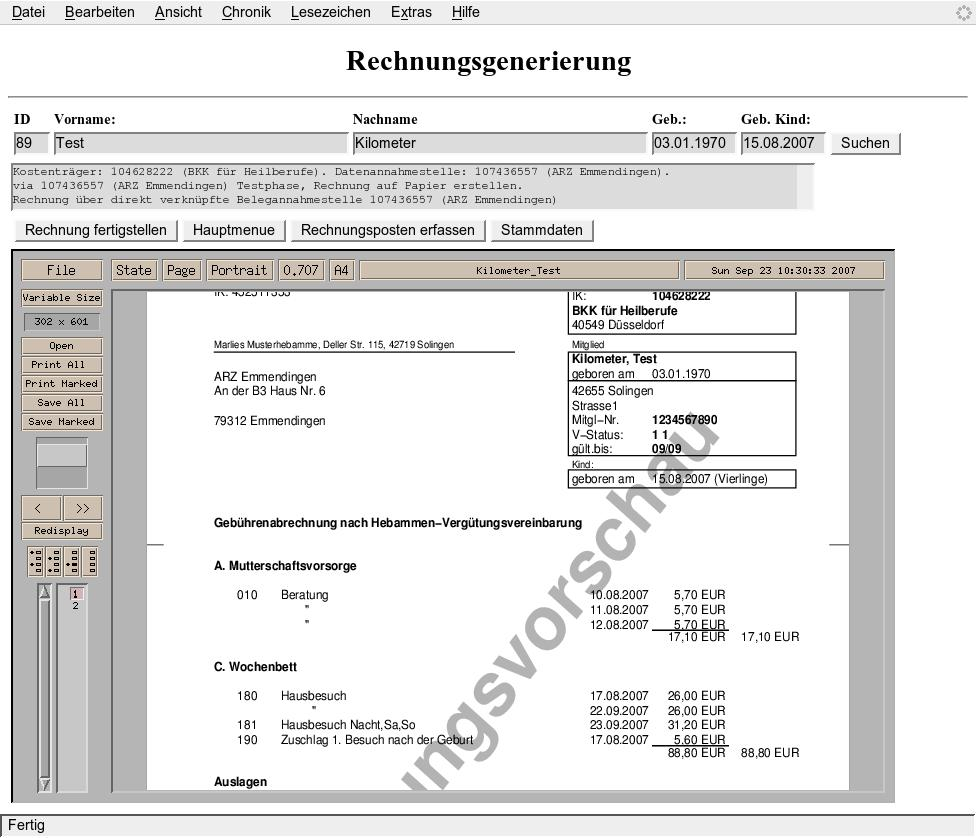
\includegraphics[width=9cm]{rechnungsgenerierung}
\caption{Rechnungsgenerierung\label{rechnungsgenerierung:fig}}
\end{figure}

Wie schon in der Kurzanleitung beschrieben, ist die Maske in zwei
Teile gegliedert. Im oberen Teil werden Daten zur Frau angezeigt,
die aktuell bearbeitet wird, sowie Informationen zur Krankenkasse.

\subsection{Daten zur Frau}
Zu den angezeigten Daten der Frau geh�ren 
die ID, Vor- und Nachname, sowie das Geburtsdatum der Frau und
des Kindes. Diese Felder k�nnen nicht erfasst werden. Soll eine andere
Frau ausgew�hlt werden, muss dies �ber den Knopf \knopf{Suchen} geschehen.
Die Beschreibung zu der Suchmaske befindet sich im Abschnitt 
\vref{frauenauswahl:abs}. Es werden keine Informationen in die Suchmaske
�bernommen. Die Suche wird unmittelbar gestartet, dabei wird nur nach
den Frauen gesucht, die einen Status ungleich erledigt besitzen.

\subsection{Informationen zur Krankenkasse}
Die Informationen zur Krankenkasse werden nur dann angezeigt, wenn es
sich um eine Kassenrechnung handelt. Ist eine Frau privat versichert 
entf�llt dieser Teil auf der Maske.

Zu jeder Krankenkasse werden die folgenden Informationen angezeigt:
\begin{enumerate} 
\item
welchem Kostentr�ger die Krankenkasse zugeordnet ist
\item
welche Datenannahmestelle die Krankenkasse, bzw. der Kostentr�ger nutzt.
\item
ob der elektronische Datenaustausch mit der Datenannahmestelle m�glich ist.
\item
ob eine Belegannahmestelle vorhanden ist, an die die Rechnung geschickt
werden muss.
\end{enumerate}

\index{elektronische Rechnung}
Es gibt verschiedene Gr�nde, warum ein elektronischer Datenaustausch mit 
einer Datenannahmestelle nicht m�glich ist. Entweder die Datenannahmestelle
ist noch nicht im Datenhaushalt von \tinyHeb\/ parametrisiert
(siehe dazu Kapitel \vref{datenannahmestellen:abs}) oder die 
Datenannahmestelle ist parametrisiert aber es liegt kein �ffentlicher
Schl�ssel der Datenannahmestelle vor (siehe dazu Kapitel \vref{anhang:pubkey}).

Ist die Datenannahmestelle parametrisiert und es liegt auch der
entsprechende Schl�ssel der Datenannahmestelle vor, ist angegeben,
in welchem Status die elektronische Rechnung verschickt wird.
\begin{enumerate}
\item
\index{Testphase}
Testphase, diese Einstellung sollte nur f�r ``Spiel'' Rechnungen genutzt
werden oder zur �berpr�fung, ob die Datennahmestelle Rechnungen
von der Rechnungsstellenden Hebamme entgegen nimmt.
\item
\index{Erprobungsphase}
Erprobungsphase, dies ist die Standardeinstellung von \tinyHeb\/ nach der
Installation der Software. In dieser Phase ist die Rechnung sowohl per
E-Mail, als auch per Papierrechnung zu verschicken. In der Regel wird man
nach drei Rechnungen zum Echtbetrieb zugelassen (siehe dazu auch
Tabelle \vref{krankenkassen302} im Anhang), wenn die Datenannahmestelle
schon den Echtbetrieb anbietet.
\item
\index{Echtbetrieb}
Echtbetrieb, nach der Zulassung zum Echtbetrieb ist es nicht mehr notwendig
Papierrechnungen an die Krankenkasse zu schicken. In der Maske wird die
Rechnungsvorschau trotzdem angezeigt, damit leicht �berpr�ft werden kann,
ob die Inhalte der Rechnung ok sind.
\end{enumerate}

\subsection{Beschreibung Kn�pfe in der Maske Rechnungsgenerierung}
Folgende Kn�pfe sind in der Maske vorhanden:

\begin{description}
\item[Rechnung fertigstellen]
\index{Rechnung!drucken}
Dieser Knopf ist nur aktiv, wenn es sinnvoll ist eine Rechnung zu erstellen,
d.h. nur wenn wirklich Rechnungsposten vorhanden sind, die abgerechnet
werden k�nnten, ist der Knopf Aktiv.

Zun�chst wird f�r jede Rechnung eine Rechnungsvorschau angzeigt. Dies
ist daran zu erkennen, dass Diagonal �ber die Rechnung der Text
Rechnungsvorschau angezeigt wird. Ist man mit dem Inhalt der Rechnung
zufrieden, kann �ber den Knopf \knopf{Rechnung fertigstellen} die
entg�ltige Rechnung produziert werden. Der Text Rechnungsvorschau
wird jetzt nicht mehr angezeigt. Alle Positionen, f�r die die
Rechnung gedruckt wurde, erhalten den Bearbeitungsstatus Rechnung,
eine weitere Bearbeitung dieser Positionen ist jetzt nicht mehr
m�glich.\marginline{\Huge\bfseries!}%

Bevor die Rechnung entg�ltig fertiggestellt wird, pr�ft \tinyHeb\/ ob 
alle notwendigen Informationen f�r den Druck der Rechnung vorhanden sind.
Ohne die folgenden Informationen ist es nicht m�glich, eine 
ordnungsgem��e Rechnung an eine Krankenkasse zu stellen:

IK Nummer der Krankenkasse, Vor- und Nachname der Frau, Geburtsdatum der
Frau und des Kindes (hier muss ggf. der errechnete Termin in den Stammdaten
erfasst werden), die Krankenversicherungsnummer und 
Versichertenstatus der Frau d�rfen nicht fehlen.

Fehlt eine dieser Informationen wird eine Fehlermeldung ausgegeben und die
Rechnung \textbf{nicht} entg�ltig fertiggestellt. Es ist dann notwendig
�ber den Knopf \knopf{Stammdaten} erneut in die Stammdatenerfassung zu 
verzweigen um die fehlenden Informationen nachzuerfassen.

Fehlen Informationen zur Anschrift der Frau, wird eine Warnmeldung ausgegeben,
ob die Rechnung trotzdem erstellt werden soll. Man kann sich in diesem 
Fall entscheiden, ob die fehlenden Informationen nacherfasst,
oder trotzdem die Rechnung erstellt werden soll.

Wenn die Rechnung erfolgreich erstellt wurde, erscheint ein
Hinweistext, wie mit der Rechnung weiter zu verfahren ist, d.h.
Rechnung ausschlie�lich ausdrucken und per Post verschicken, ggf. zus�tzlich
per E-Mail verschicken oder ausschlie�lich per E-Mail verschicken.
Dies ist Abh�ngig von der jeweiligen Krankenkasse.
Der Druck auf Papier kann f�r den Fall, das das Programm GV f�r die 
Anzeige genutzt wird, ober den Knopf \knopf{Print All} erfolgen.
Erfolgt die Vorschau, wie dies bei einer Windows Installation der Fall
ist �ber den Acrobat Reader, kann die Rechnung �ber das Druckersymbol
angestossen werden.
\item[Hauptmenue] 
�ber diesen Knopf gelangt man in die Maske Hauptmenue.
\item[Rechnungsposten erfassen] 
�ber diesen Knopf gelangt man in die Maske
zur Erfassung von Rechnungsposten. Ist eine Frau ausgew�hlt, werden deren
Daten in die Maske ``Rechnungsposten erfassen'' �bernommen.
\item[Stammdaten]
�ber diesen Knopf gelangt man in die Maske
zur Erfassung von Stammdaten. Ist eine Frau ausgew�hlt, werden deren
Daten in die Maske Stammdaten �bernommen.
\end{description}


%\section{Verschicken der Rechnung per E-Mail}
\section{Verschicken der Rechnung per E-Mail\label{elekrechnung:kap}}
\index{Rechnung!per E-Mail}
F�r das Verschicken der Rechnung per E-Mail existiert ein eigenes
Programm \textbf{xauftrag.pl}. Dieses Programm befindet sich im Verzeichnis
edifact und kann aus der Kommandozeile mit dem Befehl \verb|xauftrag.pl| gestartet
werden. Nachdem Start erscheint ein neues Fenster 
(Abbildung \vref{xauftrag:fig}).

\begin{figure}[ht]
\centering
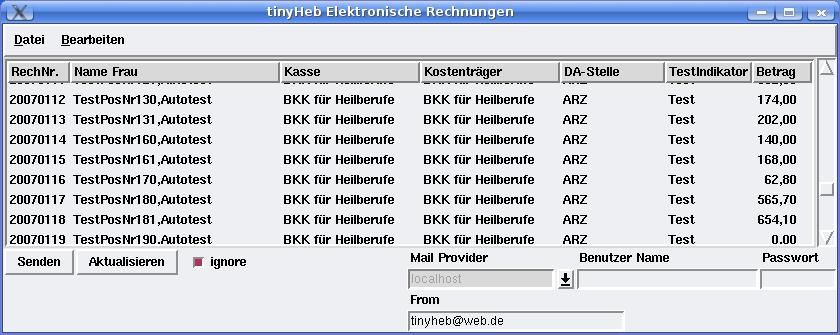
\includegraphics[width=9cm]{xauftrag}
\caption{xauftrag.pl\label{xauftrag:fig}}
\end{figure}

Das Fenster ist in zwei Bereiche geteilt. Im oberen Teil werden die
Rechnungen angezeigt, die elektronisch verschickt werden k�nnen.
Im unteren Bereich k�nnen zus�tzliche Angaben gemacht werden, die bei
der Rechnungsgenerierung genutzt werden.

\subsection{Angaben zur Rechnung}
Zu den angezeigten Daten der jeweiligen Rechnung geh�ren die
Rechnungsnummer, Vor- und Nachname der Frau, die Krankenkasse der
Frau, der Kostentr�ger der Krankenkasse, die Datenannahmestelle,
Angabe des Testindikators (Test, Erprobungsphase oder Echtbetrieb)
und der Rechnungsbetrag. Es werden nur die Rechnungen angezeigt, die
noch nicht elektronisch verschickt wurden und bei denen die M�glichkeit
zum elektronischen Rechnungsversand besteht.
Eine Rechnung kann durch Anklicken zum
elektronischen Versand ausgew�hlt werden. Sollen mehrere Rechnungen
zum Versand ausgew�hlt werden, kann dies durch Halten der Taste STRG
und Klicken auf weitere Rechnungen erreicht werden. Ausgew�hlte
Rechnungen werden in der Farbe Blau angezeigt.

\subsection{Felder und Kn�pfe}

\begin{description}
\item[Senden]
Durch Klicken auf den Knopf \knopf{Senden} werden die ausgw�hlten Rechnungen
an die entsprechenden Datenannahmestellen und die Hebamme (in Blindkopie)
verschickt.\footnote{ggf. 
ist es notwendig vor dem Senden eine Verbindung mit dem Internet herzustellen} 

Kann eine Rechnung erfolgreich verschickt werden, wird ein neues Fenster
ge�ffnet, in dem dies angezeigt wird. Das Fenster muss durch Klicken
auf den Knopf \knopf{OK} geschlossen werden, bevor weitere Rechnungen
verschickt werden k�nnen. Die Rechnung erh�lt den Status 
``Edi Rech'', f�r elektronische Rechnung und wird aus der �bersicht der
Rechnungen entfernt.

Tritt ein Fehler beim Verschicken der Rechnung auf, wird ein neues Fenster
ge�ffnet, in dem eine entsprechende Fehlermeldung angezeigt wird. Das
Versenden der Rechnungen wird abgebrochen und das Fenster muss
durch Klicken auf den Knopf \knopf{OK} geschlossen werden. 
M�gliche Ursachen f�r einen
Fehler sind z.B. eine fehlende Verbindung zum Internet (Fehlermeldung:
``The SMTP server mail.web.de was not found'') oder ein falsches
Passwort f�r die Anmeldung beim Provider (Fehlermeldung: ``Login not
accepted'').

\item[Aktualisieren]
Durch Klicken auf den Knopf \knopf{Aktualisieren} wird der Datenbestand
von \tinyHeb\/ auf alle Rechnungen durchsucht, die elektronisch verschickt
werden k�nnen. Diese Rechnungen werden angezeigt. Dies ist dann von
Interesse, wenn man weitere Rechnungen wie in Kapitel 
\vref{rechnungsgenerierung:kap} beschrieben, fertiggestellt hat 
und diese verschicken
m�chte ohne das Programm xauftrag.pl neu zu starten.

\item[ignore]
\index{Rechnung!erneut elektronisch verschicken}
Wird das Feld \feld{ignore} angew�hlt und zus�tzlich der Knopf
\knopf{Aktualisieren} gedr�ckt, werden alle Rechnungen angezeigt,
bei denen die M�glichkeit besteht, diese elektronisch zu versenden.
Dies ist unabh�ngig vom Status der Rechnung, d.h. es werden auch solche
Rechnungen angezeigt, die schon elektronisch verschickt wurden.
Rechnungen die schon beglichen sind, werden nicht angezeigt.
So ist es m�glich einzelne Rechnungen mehr als einmal zu versenden,
falls es zu Problemen beim Rechnungsversand gekommen 
ist.\footnote{dies sollte in der Regel nicht notwendig sein}

\item[Mail Provider]
\index{Mail Provider}
\index{Internet Provider}
\index{T-Online|see{Mail Provider}}
\index{Arcor|see{Mail Provider}}
\index{Web.de|see{Mail Provider}}
\index{Freenet|see{Mail Provider}}
�ber dieses Pop-Down-Menue kann der ben�tigte E-Mail Provider ausgew�hlt
werden. Als Standard Mail Provider ist auf Unix-/ Linux Systemen localhost 
angegeben, 
da \tinyHeb\/ davon ausgeht, das ein 
eigener MTA\footnote{Mail Transfer Agent} bei einer Linux
Installation �blich ist. Auf Windows Systemen wird der erste Provider,
der in der Datei \verb|.xauftragrc| angegeben ist vorgeblendet (siehe
dazu Kapitel \vref{anhang:provider}).
Sobald ein Mail Provider ausgew�hlt wurde, werden die Felder
\feld{Benutzer Name, Passwort} und \feld{From} gef�llt. Woher diese
Informationen kommen und wie zus�tzliche Provider hinterlegt werden
k�nnen ist im Anhang in Kapitel \vref{anhang:provider} beschrieben.

\item[Benutzer Name]
Dieses Feld enth�lt den Benutzer Namen, der ben�tigt wird, um sich bei
seinem Provider anzumelden. Wird kein Benutzer Name f�r die Anmeldung
ben�tigt, kann das Feld leer bleiben.

\item[Passwort]
Dieses Feld enth�lt das Passwort, welches ben�tigt wird, um sich bei seinem
Provider anzumelden. Wird kein Passwort ben�tigt, kann das Feld leer
bleiben.

\item[From]
Dieses Feld wird in die From Zeile der E-Mail �bernommen und muss
zwingend das Format name@provider.de haben. Die Datenannahmestellen
schicken die Best�tigung, ob die Rechnung empfangen wurde, an diese
E-Mail Adresse.
\end{description}

\subsection{automatische E-Mail Antwort der Datennahmestelle}
Je nach Verarbeitungsgeschwindigkeit
der Datenannahmestelle bekommt man nach ca 15 Minuten bis zu 3 Stunden eine
R�ckmeldung von der Datenannahmestelle per E-Mail, ob die Rechnung
verarbeitet werden konnte oder ein Fehler aufgetreten ist.

Sollte nach einem Tag noch keine Antwort von der Datenannahmestelle 
eigentroffen, kann dies unterschiedliche Ursachen haben, folgende Ursachen
sind bisher Evident geworden:
\begin{enumerate}
\item 
\index{Spam}
Man hat bei seinem E-Mail Provider einen Spam-Filter eingerichtet.
Die Antwort der Datennahmestelle wird als Spam Mail erkannt.
F�r diesen Fall muss der Spam Filter angepasst werden.
\item
\index{DDG}
Die Datennahmestelle ist nicht mit der Rechnungspr�fung von der
Krankenkasse beauftragt, obwohl dies in der Kostentr�gerdatei so hinterlegt
ist. Dies tritt insbesondere bei der Datennahmestelle DDG auf. Da die DDG
aber b.a.w. keinen Echtbetrieb anbieten wird ist dies nicht schlimm und
man  wird �ber den Sachverhalt schriftlich per Brief hingewiesen.
Eine Anpassung der Krankenkassendaten ist in diesem Fall notwendig.
\item 
Die Datennahmestelle erkennt die elektronische Rechnung als Spam und
verarbeitet die Rechnung nicht. Dies ist insbesondere beim ARZ-Emmendingen
der Fall, wenn die Rechnung �ber den E-Mail Provider Arcor verschickt wird.
F�r diesen Fall hilft es nur, sich einen neuen E-Mail Provider zu suchen,
da weder Arcor noch das ARZ-Emmendingen bereit sind, �nderungen ihrer
Einstellungen vorzunehmen.
In \tinyHeb\/ besteht die M�glichkeit Rechnungen �ber unterschiedliche
Provider zur verschicken, welche Einstellung dazu vorzunehmen sind, ist
im Anhang in Abschnitt \vref{anhang:provider} beschrieben. Siehe dazu
auch die Beschreibung des Feldes \feld{Mail Provider} weiter oben.
\item
\index{Signatur}
Die Rechnung wurde nicht mit einer elektronischen Unteschrift versehen
(Signatur), die Datenannahmestelle verlangt aber, dass die Rechnung
signiert ist. Dies ist z.B. bei Medent, Syntela und Autovision der Fall.
\end{enumerate}

\paragraph{Beispiel f�r eine erfolgreiche Annahmebest�tigung (hier ARZ-Emmendingen)}
\begin{verbatim}
Annahmebestaetigung 451234567 TSOL0014.auf
 Datum: 01.05.2006 11:45
 Von: Team DALE <dale@arz-emmendingen.de>
 An: 451234567 <tinyheb@web.de>
 
Diese E-Mail wurde automatisch erstellt!

Sehr geehrte Damen und Herren,

wir bestaetigen ihnen den Empfang der gesendeten Nachricht.

Eine Pruefung der von ihnen gelieferten Daten fuehrte zu dem Ergebnis:
Die Nachricht entspricht dem geforderten Aufbau und kann an die 
nachgelagerten Pruefverfahren weitergegeben werden.

Die folgenden Dateien sind in das System uebernommen worden:
TSOL0014.auf 348
TSOL0014 1641

Die Verarbeitungsergebnisse aus den Pruefstufen 1 - 4 werden separat 
protokolliert. 
Im Fehlerfall erhalten Sie hierzu separate Meldungen.

F�r etwaige Rueckfragen wurde die Datenlieferung unter der 
Referenznummer 451234567_20060501114501_0 registriert.

Mit freundlichen Gruessen

Team DALE

---

Abrechnungszentrum Emmendingen
Team DALE
An der B3 Haus Nr. 6
79312 Emmendingen
www.arz-emmendingen.de
\end{verbatim}

\paragraph{Beispiel f�r eine nicht erfolgreiche Annahmebest�tigung (hier Medent)}
\begin{verbatim}
FEHLERMELDUNG - 451234567
 Datum: 01.05.2006 10:41
 Von: 661200048 <sole@datenannahme.medent.de>
 An: 451234567 <tinyheb@web.de>
 Antwort an: 661200048 <clearing@medent.de>
 
TSOL0012.auf, 348, 20060501:1041
TSOL0012, 1553, 20060501:1041


Sehr geehrte Damen und Herren,

eine Verarbeitung Ihrer Abrechnungsdaten ist nicht moeglich, da die 
gelieferten Daten Fehler beinhalten, die zu einer Abweisung fuehren.


Daten der Anlieferung:

Uebermittelt am:         01.05.2006
Datei-Name:              TSOL0012
Bearbeitungsnummer:      981868

Erstellt am (UNB):       -
Datei-Name (UNB):        -
Datei-Nr. (UNB):         -

IK-Kostentraeger:        -
IK-Rechnungssteller:     -
Rechnungsnummer:         -
Rechnungsdatum:          -

Fehlerbeschreibung:

Es sind Fehler in der Pruefstufe 1 aufgetreten.
[2183] Es ist keine verschluesselte Nutzdatendatei vorhanden, 
oder die Nutzdatendatei ist nicht lesbar 


Ihre eventuell eingehenden Verordnungen koennen wir zur Zeit aus 
vorgenanntem Grund keine Daten zuordnen. Wir pruefen bis zu 5 Tage 
nach Eingang der Verordnungen, ob wir zwischenzeitlich die 
Daten erfolgreich annehmen konnten, andernfalls muessen wir zu unserer 
Entlastung die eingegangenen Verordnungen wieder zuruecksenden. 
Bitte reichen Sie Ihre Abrechnungsunterlagen nach erfolgter Klaerung 
wieder ein.
Falls Ihren Unterlagen eine ausfuehrliche Papierrechnung 
(incl. Einzelpreise und Positionen) beiliegt, wird diese nach Ablauf 
der 5-Tagesfrist zur Rechnungspruefung verwendet und ggf. nach Auftrag 
des Kostentraegers, eine pauschale Rechnungskuerzung nach 303 SGB V 
vorgenommen.

Mit freundlichen Gruessen,

Medent GmbH

Bei Fragen wenden Sie sich bitte an unser Team Datenaustausch unter 
Tel.: 089 / 961 77 - 511.
\end{verbatim}
Die Fehlermeldung war im o.g. Beispiel ist �bringens nicht auf \tinyHeb\/ 
zur�ckzuf�hren, sondern Medent war 2006 noch nicht in der Lage PKCS\#7
verschl�sselte Nutzdaten entgegenzunehmen\footnote{Bei Mednet m�ssen
Rechnungen verschl�sselt und signiert sein}.

\index{Rechnung!erneut elektronisch verschicken}
Ist es notwendig eine identische Rechnung ein zweitesmal zu 
verschicken --z.B. �ber einen anderen Mail Provider-- 
k�nnen durch einen
Klick auf \knopf{Ignore} und den Knopf \knopf{Aktualisieren} alle 
Rechnungen angezeigt werden, die noch nicht erledigt sind und bei denen 
es m�glich ist, diese elektronisch zu verschicken.





\section{Rechnungsbearbeitung}\label{rechnungsbearbeitung:kap}
Wie schon in der Kurzanleitung beschrieben, ist es nach Erstellung
einer Rechnung notwendig, den
Zahlungseingang zu �berwachen.
 Dazu dient die Maske Rechnungsbearbeitung. In die Maske gelangt
man aus dem Hauptmenue �ber den Link 
\verb|versandte| \verb|Rechnungen| \verb|bearbeiten|. 
Die Maske ist in zwei Teile
gegliedert. Im oberen Teil werden die Rechnungen angezeigt, die bisher
erstellt wurden, im unteren Teil k�nnen einzelne Rechnungen bearbeitet werden.

Welche Rechnungen angezeigt werden, l�sst sich durch die Auswahlbox
\feld{Anzeige Einschr�nken} beeinflussen. Es sind zwei verschiedene Werte
m�glich. Bei ``alle'', werden alle Rechnungen angezeigt. Bei
``ungleich erl.'' werden nur die Rechnungen angezeigt, die sich in einem
Status ungleich ``erl.'' befinden.

\begin{figure}[ht]
\centering
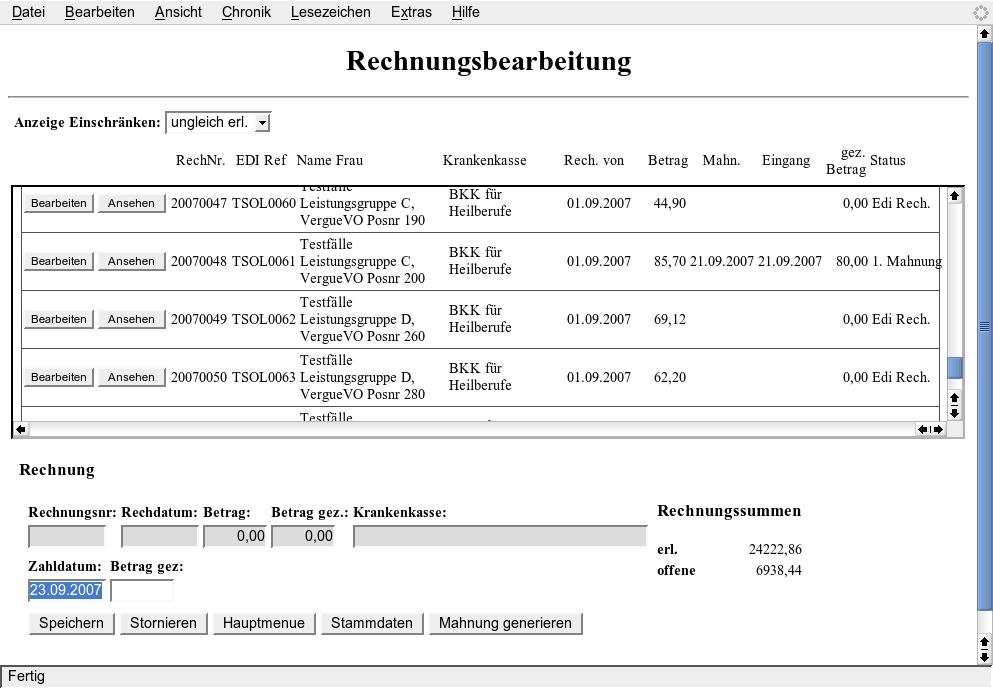
\includegraphics[width=9cm]{rechnungsbearbeitung}
\caption{Rechnungsbearbeitung\label{rechnungsbearbeitung:fig}}
\end{figure}

\subsection{�bersicht der Rechnungen}
\index{Rechnungs�bersicht}
\index{ESOL}
\index{TSOL}
Zu den angezeigten Daten einer Rechnung geh�ren die Rechnungsnummer,
die Datenaustausch\-referenz (EDI Ref),
\index{Datenaustauschreferenz}
Vor- und Nachname sowie Krankenkasse der Frau, das Datum der Rechnungsstellung,
der Rechnungsbetrag, das letzte Mahndatum -- falls die Rechnung schon
angemahnt wurde, dass Datum des letzten Rechnungseingangs, 
der gezahlte Betrag und
der Status in dem sich die Rechnung befindet. Folgende Status sind
in der Anzeige m�glich:

\begin{description}
\item[Rechnung] 
Es wurde eine Papierrechnung erstellt.
\item[Edi Rech.] 
Es wurde eine elektronische Rechnung erstellt.
\item[Teilzahl.] 
Es wurde f�r eine Rechnung eine Teilzahlung geleistet.
\item[Mahnung] 
Es wurde f�r eine Rechnung bereits eine Mahnung erstellt, 
dabei wird angegeben, wie viele Mahnung bisher erstellt wurden.
\item[Storniert]
Die Rechnung wurde storniert.
\item[erl.]
Die Rechnung wurde beglichen.
\end{description}

Neben den angezeigten Daten sind noch zwei Kn�pfe in der Anzeige vorhanden.
Durch Klicken des Knopfes \knopf{Bearbeiten} wird die entsprechende
Rechnung zur Bearbeitung ausgew�hlt und die Daten in den unteren Teil
der Maske �bernommen. Durch Klicken auf den Knopf \knopf{Ansehen} wird
ein neues Fenster ge�ffnet, in dem die original Rechnung angezeigt wird.
Falls die Rechnung elektronisch verschickt wurde, existiert in dem
neuen Fenster noch ein Pop-Down-Menue �ber das ausgew�hlt werden kann, ob 
die Papierrechnung oder die elektronische Rechnung angezeigt werden soll.
\index{elektronische Rechnung}

\subsection{Rechnung}
Im unteren Teil der Maske kann eine ausgew�hlte Rechnung bearbeitet werden.
Dies ist nur dann m�glich, wenn die Rechnung noch nicht erledigt ist. Zur
Bearbeitung einer Rechnung ist es notwendig diese im oberen Teil der Maske
durch Klicken auf den Knopf \knopf{Bearbeiten}
 auszuw�hlen. Es kann dann im Feld \feld{Zahldatum} das
Datum des Rechnungseinganges erfasst werden und im Feld
\feld{Betrag gez:} der eingegangene Betrag. F�r das Feld \feld{Zahldatum}
existieren analoge Plausipr�fungen wie f�r alle anderen Datumsfelder in der
Anwendung. F�r das Feld \feld{Betrag gez:} wird �berpr�ft, 
ob das Feld numerisch
mit maximal zwei Nachkommastellen erfasst wurde. Werden mehr Nachkommastellen
erfasst, wird eine Fehlermeldung ``Bitte numerischen Wert erfassen'' 
ausgegeben. Durch Klicken des Knopfes \knopf{Speichern} werden die erfassten
Werte in den Datenhaushalt �bernommen, dabei ist folgendes zu beachten:

\begin{enumerate}
\item
Es wird gepr�ft, ob der eingegangene Betrag kleiner ist, als der urspr�ngliche
Rechnungsbetrag. \tinyHeb\/ weisst auf diesen Sachverhalt hin und fragt,
ob die Rechnung trotzdem auf erledigt gesetzt werden soll. Beantwortet man
die Frage mit ``nein'', erh�lt die Rechnung den Status ``Teilzahlung''. 
Beantwortet man die Frage mit ``ja'', erh�lt die Rechnung den Status
``erledigt''.
\item
Es wird gepr�ft, ob der eingegangene Betrag gr��er ist, als der urspr�ngliche
Rechnungsbetrag. \tinyHeb\/ weisst auf den Sachverhalt hin und fragt, ob die
Rechnung trotzdem gespeichert werden soll. Dr�ckt man den Knopf
\knopf{Abbrechen}, kann man den erfassten Betrag korrigieren. Dr�ckt man
den Knopf \knopf{OK} wird die Rechnung auf den Status ``erledigt'' gesetzt.
\item 
Der im Feld \feld{Betrag gez:} erfasste Betrag und bisher eingegangene
Zahlungen werden summiert. Ist zum Beispiel der original Rechnungsbetrag 
127 EUR und
es geht eine Zahlung von 50 EUR ein, ist 50 EUR im Feld \feld{Betrag gez:}
zu erfassen. Nach dem Speichern erh�lt die Rechnung den Status ``Teilzahlung''.
Geht jetzt der fehlende Rechnungsbetrag von 77 EUR ein, ist im Feld
\feld{Betrag gez:} 77 EUR zu erfassen und nicht 127 EUR.
\end{enumerate}

\paragraph{Beschreibung der Kn�pfe im Menue Rechnungsbearbeitung}
\begin{description}
\item[Speichern]
Durch Klicken des Knopfes \knopf{Speichern} werden die erfassten Daten
gespeichert.
\item[Stornieren]
Durch Klicken des Knopfes \knopf{Stornieren} kann die Rechnung storniert
werden. Es werden alle Einzelposten der Rechnung auf den Status 
``in Bearbeitung'' zur�ckgesetzt. Die Rechnung erh�lt den Status storniert
und kann nicht mehr bearbeitet werden. Es k�nnen nur Rechnungen storniert
werden, bei denen noch keine Zahlung erfolgt ist.
\item[Hauptmenue]
Durch Klicken des Knopf \knopf{Hauptmenue} gelangt man in das Hauptmenue.
\item[Stammdaten]
Durch Klicken des Knopfes \knopf{Stammdaten} gelangt man in die Maske zur
Erfassung der Stammdaten. War vorher eine Rechnung zur Bearbeitung
ausgew�hlt, werden die entsprechenden Daten der Frau sofort in der
Stammdatenmaske angezeigt. War keine Rechnung zur Bearbeitung ausgew�hlt,
wird die Maske leer angezeigt.
\item[Mahnung]
Durch Klicken des Knopfes \knopf{Mahnung} gelangt man in die Maske zur
Generierung von Mahnungen. Dazu ist es notwendig vorher eine Rechnung
zur Bearbeitung auszuw�hlen.
\end{description}



\section{Mahnungsgenerierung}\label{mahnungsgenerierung:kap}
\index{Mahnung}

In diesem Kapitel wird beschrieben, wie eine Mahnung generiert werden 
kann. In die Maske Mahnungsgenerierung gelangt man aus der Maske 
Rechnungsbearbeitung (siehe \vref{rechnungsbearbeitung:kap}) indem man dort
eine Rechnung zur Bearbeitung ausw�hlt und auf den Knopf 
\knopf{Mahnung generieren} dr�ckt.

Die Maske ist in zwei Teile gegliedert. Im oberen Teil werden Daten zur Frau
angezeigt, die aktuell bearbeitet wird, sowie Informationen zur Krankenkasse.

\paragraph{Daten zur Frau}
Zu den angezeigten Daten der Frau geh�ren 
die ID, Vor- und Nachname, sowie das Geburtsdatum der Frau und
des Kindes. 


\paragraph{Informationen zur Krankenkasse}
Die Informationen zur Krankenkasse werden nur dann angezeigt, wenn es
sich um eine Kassenrechnung handelt. Ist eine Frau privat versichert 
entf�llt dieser Teil auf der Maske.

Zu jeder Krankenkasse wird angezeigt ob eine Belegannahmestelle vorhanden ist,
an die die Rechnung geschickt wird.


\subsection{Beschreibung Kn�pfe in der Maske Mahnungsgenerierung}
Folgende Kn�pfe sind in der Maske vorhanden:

\begin{description}
\item[Mahnung fertigstellen]
\index{Mahnung}

Zun�chst wird f�r jede Mahnung eine Vorschau angzeigt. Dies
ist daran zu erkennen, dass Diagonal �ber der Mahnung der Text
Mahnungsvorschau angezeigt wird. Will man die Mahnung wirklich generieren,
kann �ber den Knopf \knopf{Mahnung fertigstellen} die
entg�ltige Mahnung produziert werden. 
Der Text Mahnungsvorschau wird jetzt nicht mehr angezeigt. 
Alle Positionen, f�r die die
Mahnung gedruckt wurde, erhalten den Bearbeitungsstatus n-te Mahnung.

\item[Hauptmenue]
�ber diesen Knopf gelangt man sofort in das \tinyHeb\/ Hauptmenue.

\item[Rechnungsbearbeitung]
�ber diesen Knopf gelangt man in die Maske Rechnungsbearbeitung.

\item[Stammdaten]
�ber diesen Knopf gelangt man in die Maske Stammdaten. Die Frau mit der
entsprechenden ID wird sofort zur Bearbeitung ausgew�hlt.
\end{description}


% $Id: parameter.tex,v 1.14 2009/11/21 09:23:25 baum Exp $
% Tag $Name: tinyheb-1-6-3 $


% Copyright (C) 2004 - 2013 Thomas Baum <thomas.baum@arcor.de>
% Thomas Baum, 42719 Solingen, Germany

% This program is free software; you can redistribute it and/or modify
% it under the terms of the GNU General Public License as published by
% the Free Software Foundation; either version 2 of the License, or
% (at your option) any later version.

% This program is distributed in the hope that it will be useful,
% but WITHOUT ANY WARRANTY; without even the implied warranty of
% MERCHANTABILITY or FITNESS FOR A PARTICULAR PURPOSE.  See the
% GNU General Public License for more details.

% You should have received a copy of the GNU General Public License
% along with this program; if not, write to the Free Software
% Foundation, Inc., 59 Temple Place - Suite 330, Boston, MA 02111-1307, USA.


\chapter{Parameter\label{parameter:kap}}
\index{Parameter}
In diesem Kapitel werden die einzelenen Parameter beschrieben die
es in \tinyHeb\/ gibt. Wie neue Parameter angelegt, resp. ge�ndert werden
k�nnen und insbesondere welche Auspr�gungen sie besitzen und welche
steuernde Wirkung sie im Rest von \tinyHeb\/ haben. Die hier beschriebenen
Parameter haben eine zentrale Bedeutung f�r die Anwendung. Das hei�t
insbesondere, dass durch L�schen von bestimmten Parametern die Anwendung
nicht mehr funktionsf�hig sein kann. Also: Nur dann Parameter �ndern,
wenn man weiss, welche Auswirkung die �nderung hat.
\marginline{\Huge\bfseries!}%

\section{Parametererfassung}
Aus dem Hauptmenue gelangt man, wie schon im Kapitel 
\vref{einleitung:parameter:kap} beschrieben �ber den Link 
\verb|weitere| \verb|Wartungspunkte| in das \tinyHeb\/ 
Wartungsmenue (Abbildung \vref{parameter:wartungsmenue:fig}) und von dort �ber den
Link \verb|alle| \verb|Parameter| in die Maske zur Parameterpflege 
(Abbildung \vref{parameterpflege:fig}).
%
\begin{figure}[h]
\centering
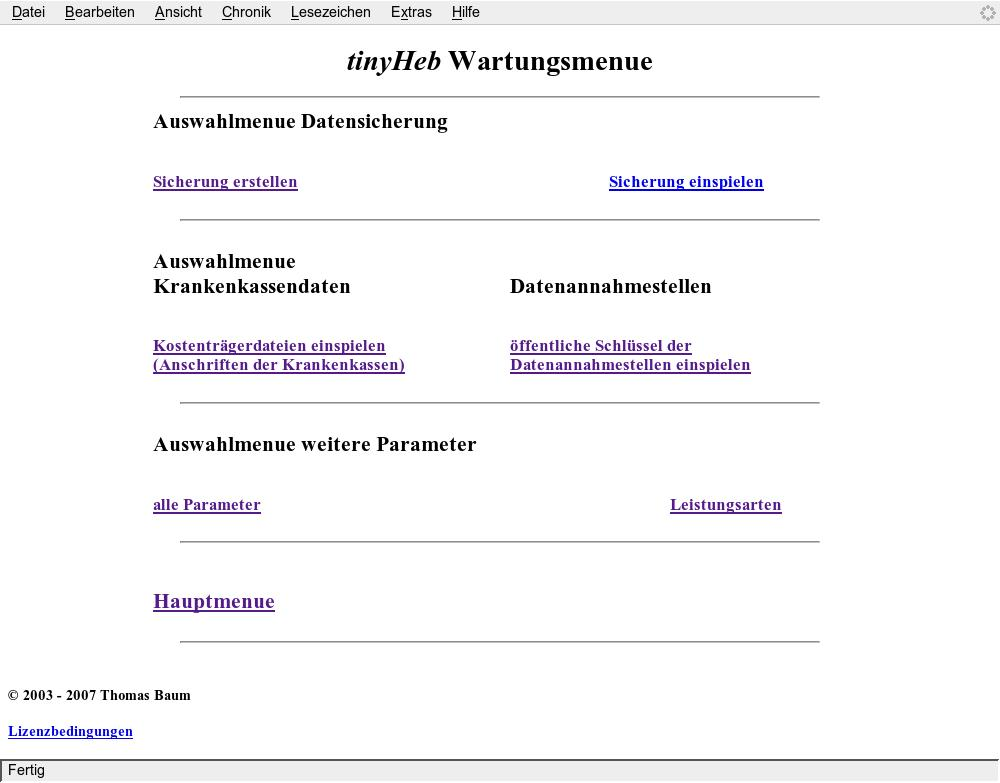
\includegraphics[width=80mm]{wartungsmenue}
\caption{\tinyHeb\/ Wartungsmenue \label{parameter:wartungsmenue:fig}}
\end{figure}
%
\begin{figure}[ht]
\centering
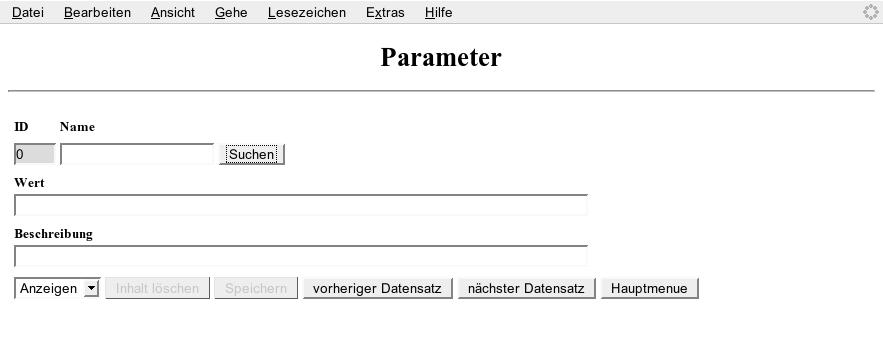
\includegraphics[width=80mm]{parameterpflege}
\caption{Parameterpflege\label{parameterpflege:fig}}
\end{figure}
%

Die Maske zur Pflege der Parameter ist relativ simple gestaltet. 
Folgende Felder sind in der Maske vorhanden:

\begin{description}
\item[ID] Dieses Feld enth�lt die interne ID zum angezeigten Parameter, es wird
automatisch gef�llt und kann nicht ge�ndert oder erfasst werden.
\item[Name] Name des Parameters, �ber diesen Namen wird in der 
Anwendung auf den Wert des Parameters zugegriffen. Es ist auf korrekte 
Schreibweise (insb. Gro�-/ Kleinschreibung) zu achten, da sonst nicht
auf den Wert zugegriffen werden kann. Es kann zwischen zwei Arten von
Namen unterschieden werden, eindeutige Namen, z.B. RECHNR, oder Namen, die 
h�ufiger vorkommen k�nnen, z.B. BEGRUENDUNG. Es exisiert keinerlei
Plausipr�fung f�r den Inahlt des Feldes.
\item[Wert] Dieses Feld enth�lt den Wert zu dem im Feld \feld{Namen}
bezeichneten Parameter. Es exisiert keinerlei Plausipr�fung f�r den 
Inahlt des Feldes.
\item[Beschreibung] 
Dieses Feld kann eine Beschreibung zu dem Parameter
enthalten, wie z.B. ``Z�hler f�r Rechnungsnummer'' f�r das Feld RECHNR.
Es exisiert keinerlei Plausipr�fung f�r den Inahlt des Feldes.
\end{description}

\subsection{Beschreibung der Kn�pfe im Parametermenue}
\begin{description}
\item[Suchen] Mit dem Knopf \knopf{Suchen} kann eine weitere Maske ge�ffnet
werden, �ber die Parameter gesucht werden k�nnen. Die Beschreibung zu der
Suchmaske befindet sich in Abschnitt \vref{parameterauswahl:abs}.
In diese Maske werden die Werte aus den Feldern \feld{Name, Wert} sowie
\feld{Beschreibung} �bernommen und die Suche unmittelbar gestartet.
\item[Inhalt l�schen] Der Knopf \knopf{Inhalt l�schen} ist nur dann
Aktiv, wenn in dem
Pop Down Menue vor dem Knopf der Wert Neu ausgew�hlt wurde. Wird der Knopf
gedr�ckt, werden alle Felder der Maske auf ihren initalen Wert gesetzt und das
Pop Down Menue springt auf den Wert Anzeigen,
\item[Speichern/ L�schen] Der Knopf \knopf{Speichern} ist nur dann aktiv,
wenn im Auswahlmenue entweder der Wert Neu oder �ndern gew�hlt wird. 
\par
Falls Neu 
ausgew�hlt wurde, wird ein neuer Parametersatz in der Datenbank gespeichert
und das Pop Down Menue springt auf den Wert Anzeigen. Es finden wie
schon bei der Erfassung der Felder beschrieben keine Plausibilit�ten
Pr�fungen statt.\par
Falls �ndern gew�hlt wurde, wird der Datensatz, der sich in der Datenbank
befindet mit den angezeigten Werten �berschrieben und das Pop Down Menue
springt auf den Wert Anzeigen. 
Es finden, wie
schon bei der Erfassung der Felder beschrieben, keine Plausibilit�ten
Pr�fungen statt.\par
Falls im Pop Down Menue L�schen ausgew�hlt wurde, erh�lt der Knopf die
Beschriftung L�schen. Durch Dr�cken des Knopfes wird der Datensatz aus der
Datenbank gel�scht. Es findet keine Plausipr�fung statt.
Wurde der Datensatz erfolgreich gel�scht, werden
alle Felder der Maske auf ihren Initial-Wert gesetzt und das Auswahlmenue
steht auf den Wert Anzeigen.
\item[vorheriger Datensatz] Dieser Knopf ist nur dann aktiv, wenn der Wert
des Pop Down Menues auf Anzeigen steht. Durch Dr�cken des Knopfes wird auf
den vorherigen Datensatz in der Datenbank gesprungen. Der vorherige Datensatz
ist derjenige mit der n�chst kleineren ID, als der aktuell angezeigte. Ist
man am ersten Datensatz angekommen, bleibt dieser in der Maske erhalten.
\item[n�chster Datensatz] Dieser Knopf ist nur dann aktiv, wenn der Wert
des Pop Down Menues auf Anzeigen steht. Durch Dr�cken des Knopfes wird auf
den n�chsten Datensatz in der Datenbank gesprungen. Der n�chste Datensatz
ist derjenige mit der n�chst h�heren ID, als der aktuell angezeigte. Ist
man am letzten Datensatz angekommen, bleibt dieser in der Maske erhalten.
\item[Hauptmenue] �ber diesen Knopf gelangt man in die Maske Hauptmenue.
Dabei ist zu beachten, dass nicht �berpr�ft wird, ob �nderungen oder Neu
erfasste Daten gespeichert wurden. Es wird sofort in die Maske Hauptmenue
gesprungen.
\end{description}

Sind alle Felder erfasst, k�nnen die Daten gespeichert werden. Dazu ist
es notwendig im Pop Down Menue unten links den Wert 'Neu' auszuw�hlen.
Sobald dies geschehen ist, wird der Knopf \knopf{Speichern} aktiv 
geschaltet. Dr�ckt man jetzt den Knopf \knopf{Speichern} werden die Daten
zu dem Parameter permanent abgelegt. Nach dem Speichern wird die Auswahl im 
Pop Down Menue unten links auf den Wert 'Anzeigen' gesetzt.




\section{Parameterauswahl\label{parameterauswahl:abs}}
In diesem Absatz ist beschrieben, wie Parameter im Datenbestand gesucht und
ausgew�hlt werden k�nnen. Der  Aufruf der Maske erfolgt aus der 
Parametererfassung (siehe Seite \pageref{parameterpflege:fig}) 
�ber den Knopf \knopf{Suchen}. 
Klickt man auf den Knopf \knopf{Suchen} wird ein neues Fenster mit der
�berschrift ``Parameter suchen'' ge�ffnet\footnote{sollte das Fenster 
noch ge�ffnet sein, wird es in den Vordergrund des Bildschirms geholt.} 
(siehe Abbildung \vref{parameterauswahl:fig}). �ber die Felder \feld{Name,
Beschreibung, Wert} ist es m�glich die
Suchkrieterien vorzugeben, d.h. es werden bei der Suche nur die Parameter
ausgegeben, bei denen alle vorgegebenen Werte vorhanden sind. Dabei ist
folgendes f�r die Felder zu beachten:

\begin{figure}[ht]
\centering
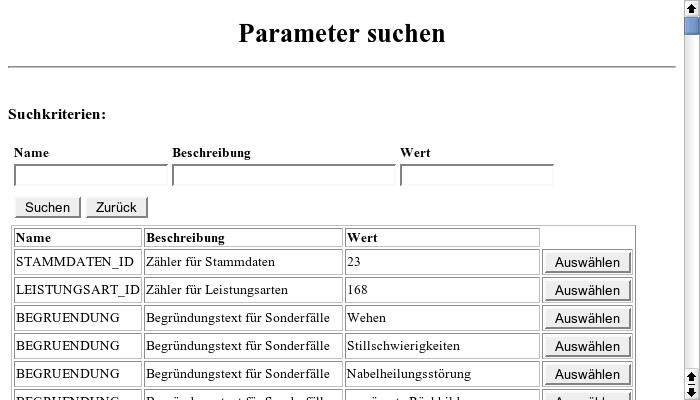
\includegraphics[width=9cm]{parameterauswahl}
\caption{Parameterauswahlmaske\label{parameterauswahl:fig}}
\end{figure}

\begin{description}
\item[Name] Es wird nur nach den Parametern gesucht, bei denen der Name
einen Teil des Feldes enth�lt.
Wird z.B. im Feld \feld{Name} ``HEB'' erfasst,
w�rde HEB\_VORNAME, HEB\_NACH\-NAME, HEB\_PLZ, usw. ermittelt werden.
\item[Beschreibung] Es wird nur nach den Parametern gesucht, bei denen die
Beschreibung mit dem Feldinhalt beginnt. Wird z.B. im Feld 
\feld{Beschreibung} ``Z�hler'' erfasst,
w�rden alle Parameter, die mit ``Z�hler'' beginnen ermittelt werden, d.h.
``Z�hler f�r Stammdaten'', ``Z�hler f�r Leistungsarten'', usw.
\item[Wert] Es wird nur nach den Parametern gesucht, die diesen Wert
enthalten.
\end{description}

Ist der Aufruf der Maske aus der Maske Parameter
erfolgt, werden die Werte Name, Wert und Beschreibung
in die Suchkriterien �bernommen und die Suche wird unmittelbar gestartet.
Die Felder k�nnen jederzeit mit neuen Suchkriterien gef�llt und die Suche
�ber den Knopf \knopf{Suchen} gestartet werden.

Das Ergebnis der Suche wird unmittelbar unter den Suchkriterien ausgegeben.
Es werden die Daten zu Name, Beschreibung und Wert ausgegeben.

�ber den Knopf \knopf{Ausw�hlen} werden die Daten des Parameters in die Maske
�bernommen, aus der die Suchfunktion aufgerufen wurde. Die Maske
``Parameter suchen''
wird danach geschlossen.

Falls keine Parameter den gew�nschten Suchkriterien entsprechen, kann entweder
durch Klicken des Knopfes \knopf{Zur�ck} die Maske ``Parameter suchen''
geschlossen werden, oder es k�nnen andere Suchkriterien erfasst werden.

\section{Beschreibung der einzelnen Parameter}

\subsection{Angaben zur Hebamme\label{parm:heb:abs}}
\index{Angaben zur Hebamme}
\index{Hebamme}
\index{Hebamme!IK-Nummer}
\index{Hebamme!Steuernummer}
\index{Steuernummer|see{Hebamme!Steuernummer}}
\index{Beleghebamme}
Die in Tabelle \vref{angaben_hebamme} beschriebenen Parameter lassen 
sich neben der Pflege in der Maske Parameter auch �ber die Maske
Angaben zur Hebamme �ndern (siehe Abbildung \vref{angaben_zur_hebamme:fig}),
die �ber einen Link mit der identischen
Bezeichnung aus dem Hauptmenue erreichbar ist. Diese Maske enth�lt
alle relevanten Daten auf einen Blick.

\begin{figure}[H]
\centering
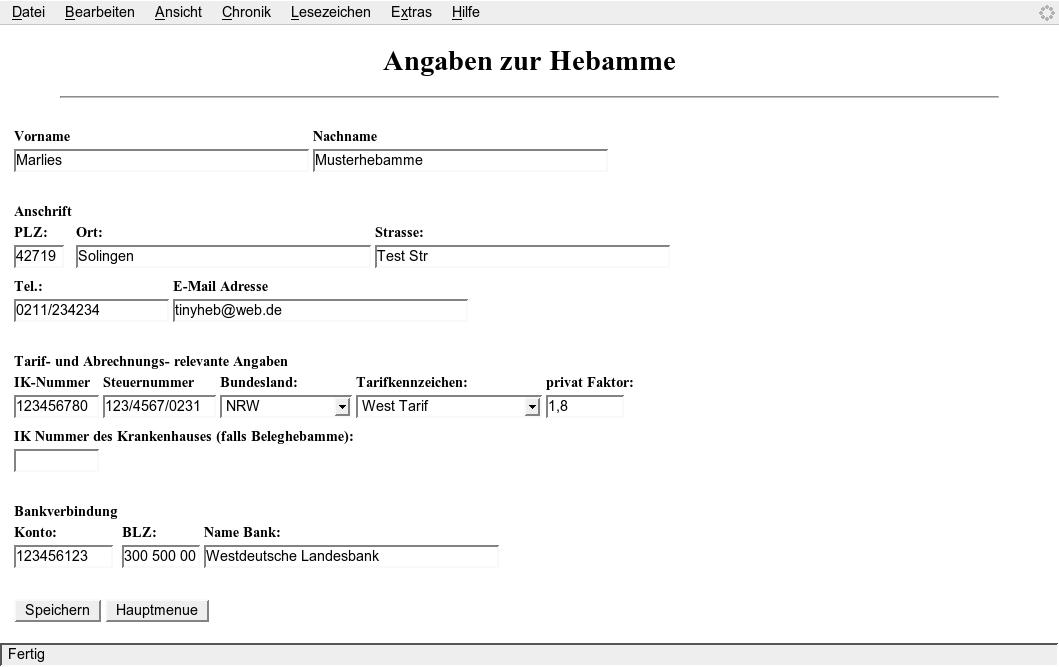
\includegraphics[width=80mm]{angaben_zur_hebamme}
\caption{Maske Angaben zur Hebamme\label{angaben_zur_hebamme:fig}}
\end{figure}


\bottomcaption{Angaben zur Hebamme\label{angaben_hebamme}}
\tablehead
{\hline \bfseries Name&\bfseries Beschreibung\\ \hline}

\tabletail
{\hline \multicolumn{2}{r}{\emph{Fortsetzung auf der n�chsten Seite}}\\}

\tablelasttail{\hline}

\begin{mpsupertabular}{|p{3.9cm}p{9.0cm}|}
%\firsthline
%\textbf{Name}&\textbf{Beschreibung}
%\tabularnewline\hline
HEB\_VORNAME&
Vorname der Hebamme. Wird in die elektronische Rechnung �bernommen und
auf der Papierrechnung mit angedruckt.
\tabularnewline\hline
HEB\_NACHNAME&
Nachname der Hebamme. Wird in die elektronische Rechnung �bernommen und
auf der Papierrechnung mit angedruckt.
\tabularnewline\hline
HEB\_TEL&
Telefonnumer der Hebamme. Wird in die elektronische Rechnung �bernommen und
auf der Papierrechnung mit angedruckt.
\tabularnewline\hline
HEB\_STRASSE&
Stra�e der Anschrift der Hebamme. Wird auf der Papierrechnung mit angedruckt.
\tabularnewline\hline
HEB\_PLZ&
Postleitzahl der Anschrift der Hebamme. Wird auf der Papierrechnung mit angedruckt.
\tabularnewline\hline
HEB\_ORT&
Ort der Anschrift der Hebamme. Wird auf der Papierrechnung mit angedruckt.
\tabularnewline\hline
HEB\_IK&
\index{Hebamme!IK-Nummer}
IK Nummer der Hebamme. Wird in die elektronische Rechnung �bernommen und
auf der Papierrechnung mit angedruckt. Die IK Nummer wird in die Betreff
Zeile der E-Mail und in die ``Absender'' Zeile �bernommen.
\tabularnewline\hline
HEB\_Konto&
Kontonummer der Hebamme. Wird auf der Papierrechnung mit angedruckt.
\tabularnewline\hline
HEB\_BLZ&
Bankleitzahl der Kontoverbindung der Hebamme. Wird auf der Papierrechnung
mit angedruckt.
\tabularnewline\hline
HEB\_NAMEBANK&
Bezeichnung der Bank, der Kontoverbindung der Hebamme. Wird auf der
Papierrechnung mit angedruckt.
\tabularnewline\hline
HEB\_TARIFKZ&
\index{Tarifkennzeichen}
Tarifkennzeichen der Hebamme gem�� \cite{schluessel}[Abschnitt 8.1.5.2].
F�r Hebammen in Westdeutschland muss 24 eigetragen werden, f�r Hebammen
in Ostdeutschland 25, oder man benutzt 00 f�r bundeseinheitlichen Tarif.
Wird f�r die Generierung der Rechnung ben�tigt und
in die elektronische Rechnung �bernommen.
\tabularnewline\hline
HEB\_EMAIL&
E-Mail Adresse der Hebamme, zwingend im Format \nolinkurl{name@provider.de}.
Wird in die ``Absender'' Zeile hinter die IK Nummer �bernommen.
An diese E-Mail Adresse wird zus�tzlich ein Blindkopie der Rechnung aus 
Dokumenationsgr�nden geschickt.
\tabularnewline\hline
HEB\_STNR&
\index{Steuernummer}
Steuernummer der Hebamme im Format 123/4568/891. Dieser Wert wird, wenn
vorhanden in die Fu�zeile der Rechnung gedruckt und in die elektronische
Rechnung �bernommen. In der elektronischen Rechnung werden die / durch
Leerzeichen ersetzt.
\tabularnewline\hline
HEB\_BUNDESLAND&
Bundesland in dem die Hebamme t�tig ist. Zur Zeit sind NRW, Bayern,
Hessen, Hamburg, Th�ringen, Rheinland-Pfalz und
\index{Bundesland}
Niedersachsen implementiert. Dieser Parameter wird dazu genutzt, die
korrekte Privat-Geb�hrenordnung zu ermitteln. In diesem Zusammenhang
ist auch die korrekte Pflege des Parameters PRIVAT\_FAKTOR zu beachten,
die im n�chsten Abschnitt beschrieben ist.
Zu einem sp�teren Zeitpunkt
wird �ber diesen Parameter auch die Ermittlung der individuellen
Feiertage erfolgen.
\tabularnewline\hline
HEB\_IK\_BELEG\_KKH&
In diesem Feld wird die IK Nummer des Krankenhauses angegeben, in dem die
Hebamme als Beleghebamme\index{Beleghebamme} t�tig ist. 
Ist die Hebamme nicht als Beleghebamme
t�tig, darf in diesem Feld nichts erfasst werden\footnote{ab
01.02.2008 wird dieses Feld in die elektronischen Rechnungen �bernommen}.
\tabularnewline\hline

\end{mpsupertabular}
 

\subsection{Programmsteuerungsparameter}\label{programmsteuerungsparameter}

\begin{table}[H]
%\centering
\begin{tabular}{|p{3cm}p{11cm}|}
\firsthline
\textbf{Name}&\textbf{Beschreibung}
\tabularnewline\hline
BEGRUENDUNG&
enth�lt Begr�ndungstexte, die bei bestimmten Leistungsarten notwendig
sind. Z.B. Wehen oder Stillschwierigkeiten. Dieser Parameter kann mehrfach
vorkommen. Enth�lt der Wert den Inhalt ``Anordnung'' muss das entsprechende
Rezept mit der Rechnung verschickt werden. Bei Rechnungen die ausschlie�lich
elektronisch �bermittelt werden, wird ein sogenannter Urbeleg generiert. In
diesem Urbeleg muss die Anzahl der �bermittelten Belege angegeben werden.
Jeder Rechnungsposten, der den Wert ``Anordnung'' enth�lt wird gez�hlt.
Eine Erfassung von Rechnungsposten bei denen eine �rztliche Anordnung
gem�� HebGo notwendig ist, ist nur m�glich, wenn o.g. Begr�ndung ausgew�hlt
wird.
\tabularnewline\hline
BELEGE&
Steuert, ob die Papierrechnungen an die Krankenkasse (Wert 0) oder
an die in der Kostentr�gerdatei \cite{ktrdat} angegebenen 
Belegannahmestellen geschickt werden (Wert  1, dies ist die 
Standardeinstellung).
\tabularnewline\hline
PRIVAT\_FAKTOR&
Mit welchem Wert m�ssen die Rechnungsposten bei privat Versicherten 
\index{Privatfaktor}
multipliziert werden. In Nordrhein-Westfalen und Bayern z.B. 1,8 in 
Niedersachsen, Hamburg oder Hessen 2,0. Wichtig ist,
dass dieser Wert mit einem . (Punkt) und nicht mit einem , (Komma)
erfasst wird.
\tabularnewline\hline
\lasthline
\end{tabular}
\caption{Programmsteuerungsparameter\label{programmsteuerung_parm}}
\end{table}



\subsection{Z�hler}

\begin{table}[H]
%\centering
\begin{tabular}{|p{3.5cm}p{10cm}|}
\firsthline
\textbf{Name}&\textbf{Beschreibung}
\tabularnewline\hline
STAMMDATEN\_ID&
Z�hler f�r Stammdaten. Wird immer dann um eins erh�ht, wenn in der Maske 
Stammdaten eine Kundin neu angelegt wird. Der Parameter enth�lt die
letzte vergebene ID und sollte nicht manuell ge�ndert werden.
\tabularnewline\hline
LEISTUNGSART\_ID&
Z�hler f�r Leistungsarten. Wird immer dann um eins erh�ht, wenn in der
Maske Leistungsarten eine neue Leistungsart gespeichert wird, bzw. eine
bestehende Leistunsart ge�ndert wird. Der Parameter enth�lt die
letzte vergebene ID und sollte nicht manuell ge�ndert werden.
In der Tabelle der Leistungsarten
sind u.a. alle Positionsnummern der HebGV mit den entsprechenden Preisen
hinterlegt.
\tabularnewline\hline
LEISTUNG\_ID&
Z�hler f�r Leistungsdaten. Wird immer dann um eins erh�ht, wenn in der
Maske Rechnungserfassung neue Leistungen gespeichert werden, bzw. eine
bestehende Position ge�ndert wird. Der Parameter enth�lt die
letzte vergebene ID und sollte nicht manuell ge�ndert werden.
\tabularnewline\hline
RECHNR&
Z�hler \index{Rechnungsnummer} f�r die Rechnungsnummer. 
Wird immer dann um eins erh�ht, wenn eine
Rechnung �ber den Knopf \knopf{Rechnung fertigstellen} in der Maske 
Rechnungsgenerierung fertiggestellt wird. Der Parameter enth�lt die letzte
vergebene Rechnungsnummer. Soll am Beginn eines Jahres dieser Z�hler
auf einen neuen Start Wert gesetzt werden, ist dieser Wert auf z.B. 20070000
zu setzen. Die Rechnungsnummer muss unbedingt numerisch erfasst werden.
\tabularnewline\hline
KALENDER\_ID&
Z�hler f�r Feiertage. Wird immer dann um eins erh�ht, wenn in der Maske 
Feiertage ein neuer Feiertag angelegt wird. Der Parameter enth�lt die
letzte vergebene ID und sollte nicht manuell ge�ndert werden.
\tabularnewline\hline
PARM\_ID&
Z�hler f�r Parameter. Wird immer dann um eins erh�ht, wenn in der Maske 
Parameter ein neuer Parameter angelegt wird. Der Parameter enth�lt die
letzte vergebene ID und sollte nicht manuell ge�ndert werden.
\tabularnewline\hline
\lasthline
\end{tabular}
\caption{Z�hler\label{zaehler_parm}}
\end{table}



\subsection{Datenannahmestellen}\label{datenannahmestellen:abs}
\index{Datenannahmestelle}
\index{PKCS\#7}
F�r die Pflege der Parameter zu den einzelnen Datenannahmestellen
existiert seit Version 0.10.0 eine eigene Maske. Diese Maske kann aus dem
Hauptmenue �ber den Link \verb|Parameter| \verb|der| \verb|Datenannahmestellen|
erreicht werden (siehe Abbildung \vref{parameter:datenannahmestellen:fig}).

Folgende Felder sind in der Maske enthalten.
\begin{description}
\item[IK-Nummer Name] 
�ber dieses Feld kann die zu bearbeitende Datenannahmestelle 
ausgew�hlt werden.
\item[Status (Testindikator)]
\index{Testphase}
Das Feld \feld{Status (Testindikator)} entspricht dem Parameter IK,
\item[E-Mail]
das Feld \feld{E-Mail} entspricht dem Parameter MAIL,
\item[Verschl�sselung]
\index{Verschl�sselung}
das Feld \feld{Verschl�sselung} entspricht dem Parameter SCHL,
\item[Signatur]
\index{Signatur}
das Feld \feld{Signatur} entspricht dem Parameter SIG und
\item[Datenaustauschreferenz]
das Feld \feld{Datenaustauschreferenz} entspricht dem Parameter DTAUS.
\end{description}

Eine genaue Beschreibung der Maske folgt in einem der n�chsten Releases.

\begin{figure}[ht]
\centering
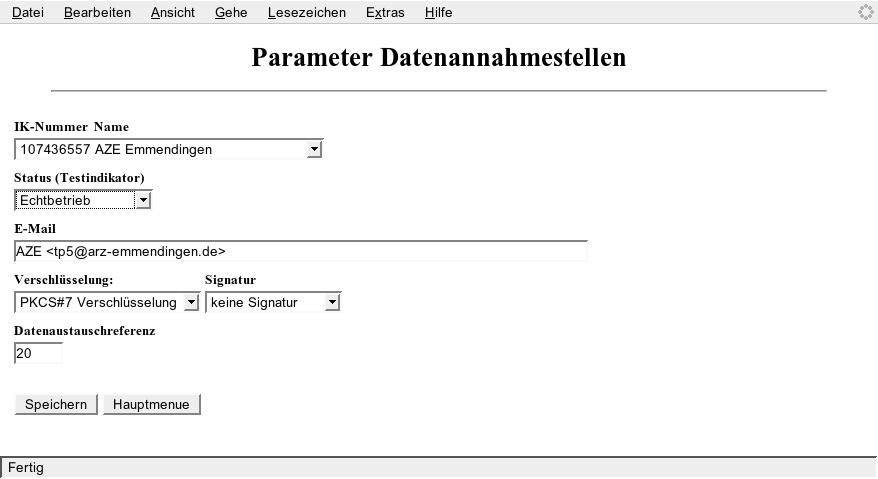
\includegraphics[width=80mm]{parameter_datenannahmestellen}
\caption{Maske Parameter der Datenannahmestellen\label{parameter:datenannahmestellen:fig}}
\end{figure}

F�r jede Datenannahmestelle sind f�nf Parameter zu erfassen, die in den
folgenden Tabellen beschrieben sind. Die Parameter enden alle mit der
IK Nummer der Datenannahmestelle, z.B. DTAUS104212516 oder 
IK104212516 bei Datenannahmestelle 
104212516. Bei Datenannahmestelle 661200093 w�re der Name des Parameters
IK661200093.

\begin{minipage}{14cm}
\begin{tabular}{|p{1cm}p{12cm}|}
\firsthline
\textbf{Name}&\textbf{Beschreibung}
\tabularnewline\hline
IK&
Mit welchen Status wird der Datenaustausch mit der Datenannahmestelle
durchgef�hrt. Name des Parameters z.B. IK104212516 bei Datenannahmestelle 
104212516. Sobald dieser Parameter f�r eine Datenannahmestelle gepflegt
ist, wird die Datenannahmestelle im Menue Rechnungsgenerierung angezeigt.
Wichtig ist es alle Parameter der Datenannahmestelle zu pflegen, um eine
korrekte elektronische Rechnung zu generieren. Trotz Pflege aller Parameter
besteht die M�glichkeit, dass eine Datennahmestelle in der Maske
Rechnungsgenerierung nicht als solche angezeigt wird, dies ist dann der
Fall, wenn kein �ffentlicher Schl�ssel der Datennahmestelle vorhanden ist.
\begin{enumerate}
\item[00] 
\index{Testphase}
Testphase gem�� \cite{pruefverfahren}. Diese Phase ist nur f�r
Softwareentwickler oder zum Test der Anwendung notwendig. Sie kann
auch genutzt werden, um zu pr�fen, ob Rechnung akzeptiert werden.
\item[01] 
\index{Erprobungsphase}
Erprobungsphase gem�� \cite{pruefverfahren}. Dies ist die
Standardeinstellung in \tinyHeb\/ nach der Installation.
Mit jeder Datenannahmestelle muss die Erprobungsphase durchlaufen 
werden\footnote{mit fast jeder -- erreicht man die Zertifizierung bei einer AOK,
 so wird dies allen anderen AOKen in Deutschland mitgeteilt.}. In dieser
Phase m�ssen sowohl Papier- wie auch elektronische Rechnungen gestellt
werden. Auf der Papierrechnung wird ein entsprechender Hinweis mit
ausgegeben, dass diese Rechnung auch per E-Mail verschickt wurde. Dies
wird von einigen Datenannahmestellen so gew�nscht. Die Erprobungsphase
ist beendet, wenn der Leistungserbringer von der Krankenkasse zum 
Echtverfahren zugelassen wird \cite{pruefverfahren}.
\item[02] 
\index{Echtverfahren}
Echtverfahren gem�� \cite{pruefverfahren}. Im Echtverfahren
ist es nicht mehr notwendig Rechnungen auf Papier zu verschicken.
Belege wie z.B. f�r Auslagen oder auch Rezepte sind weiterhin an die 
in der Kostentr�gerdatei genannten 
Belegannahmestellen zu schicken. In \tinyHeb\/ wird weiterhin eine
Papierrechnung erstellt. Auf dieser ist vermerkt, dass diese ausschlie�lich
f�r die eigenen Unterlagen ist. Sind Urbelege zu verschicken, wird im Anschlu�
an die Rechnung zus�tzlich ein Formblatt f�r Begleitzettel f�r Urbelege 
generiert \cite{urbelege}. \index{Urbeleg} 
Auf diesem Formblatt kann eingetragen werden,
wie viele Urbelege verschickt werden.
\end{enumerate}
\tabularnewline\hline
\lasthline
\end{tabular}
\captionof{table}{Parameter f�r Datenaustausch\label{datenaus_parm_ik}}
\end{minipage}



\begin{minipage}{14cm}
%\centering
\begin{tabular}{|p{1cm}p{12cm}|}
\firsthline
\textbf{Name}&\textbf{Beschreibung}
\tabularnewline\hline
SCHL&
\index{Verschl�sselung}
Mit welchem Verschl�sselungsverfahren wird der Datenaustausch mit 
der Datennahmestelle durchgef�hrt, z.B. Name des Parameters SCHL661200093.
\begin{enumerate}
\item[00] Es wird keine Verschl�sselung durchgef�hrt. Sobald echte Daten
�ber das Internet ausgetausch werden, ist man gem�� Datenschutzgesetz dazu
verpflichtet, die Daten zu verschl�sseln. Das hei�t, dieser Wert sollte nur
f�r Testzwecke mit ``Spieldaten'' gew�hlt werden.
\item[02] Verschl�sselung im PEM Verfahren. Dieses Verfahren ist nur bei
den gesetzlichen Krankenkassen in Deutschland gebr�uchlich und wird von
\tinyHeb\/ nicht unterst�tzt. Bei diesem Verfahren wird von den 
Krankenkassen mit einer Schl�ssell�nge von 768 Bit gearbeitet. Diese L�nge
wird vom BSI nicht mehr als sicher angesehen.
\item[03] 
\index{PKCS\#7}
Verschl�sselung im PKCS\#7 Format. Dieses Verfahren ist der Standard
f�r \tinyHeb\/ und wird der zuk�nftige Standard im Datenaustausch mit den
gesetzlichen Krankenkassen werden.
\end{enumerate}
\tabularnewline\hline
\lasthline
\end{tabular}
\captionof{table}{Parameter f�r Datenaustausch (Verschl�sselung)\label{datenaus_parm_schl}}
\end{minipage}



\begin{minipage}{13.0cm}
\begin{tabular}{|p{1.4cm}p{11.8cm}|}
\firsthline
\textbf{Name}&\textbf{Beschreibung}
\tabularnewline\hline
SIG&
\index{Signatur}
\index{Signieren|see{Signatur}}
Mit welchem Signaturverfahren wird der Datenaustausch mit 
der Datenannahmestelle durchgef�hrt, z.B. Name des Parameters SIG661200093
bei Datenannahmestelle 661200093.
\begin{enumerate}
\item[00] Die Rechnung wird mit keiner Signatur versehen. Die ist der
Standard in \tinyHeb, da aktuell die Datenannahmestellen nicht in der
Lage sind, signierte Rechnungen entgegenzunehmen. Dies entspricht nach
Meinung des Autors nicht dem SigG. Entsprechende Rechnung werden aber
anstandslos gezahlt.
\item[02] Signierung im PEM Verfahren. Dieses Verfahren ist nur bei
den gesetzlichen Krankenkassen in Deutschland gebr�uchlich und wird von
\tinyHeb\/ nicht unterst�tzt.
\item[03] 
\index{PKCS\#7}
Signierung im PKCS\#7 Format. Dieses Verfahren ist in 
\tinyHeb\/ implementiert. Um eine Rechnung signieren zu k�nnen, ist es
notwendig �ber ein eigenes Zertifikat zu Verf�gen, welches von der 
ITSG \cite{itsg} erteilt wird. Im Anhang in Abschnitt
\ref{anhang:eigenes_cert} ist beschrieben, wie Verfahren werden muss, um
ein solches Zertifikat zu erlangen. Dieser Abschnitt sollte im Detail
gelesen werden, da von der ITSG wenig Hilfe zu erwarten ist, wenn nicht
deren ``Tool'' D* genutzt wird.
\end{enumerate}
\tabularnewline\hline
\lasthline
\end{tabular}
\captionof{table}{Parameter f�r Datenaustausch (Signatur)\label{datenaus_parm_sig}}
\end{minipage}


\begin{minipage}{13.5cm}
\begin{table}[H]
\begin{tabular}{|p{1.3cm}p{11.9cm}|}
\firsthline
\textbf{Name}&\textbf{Beschreibung}
\tabularnewline\hline
MAIL&
An welche Mail Adresse m�ssen die Rechnungen bei der Datenannahmestelle 
geschickt werden, z.B. Name des Parameters MAIL661200093
bei Datenannahmestelle 661200093.
Hier muss die komplette E-Mail Adresse in Format: Name <email.datenannahmstelle.de> stehen.
D.h. f�r die Datenannahmestelle 661200093 Medent muss der Parameter folgenden
Wert enthalten: MEDENT <sole@datenannahme.medent.de>
\tabularnewline\hline
DTAUS&
Enth�lt die Datenaustauschreferenz f�r diese Datenannahmestelle, z.B. Name
des Parameters DTAUS661200093. Diese Parameter enth�lt die n�chste zu
vergebene Austauschreferenz. Der Wert wird nachdem eine Rechnung
elektronisch verschickt wurde um eins erh�ht. Wird eine neue
Datenannahmestelle parametrisiert, sollte dieser Wert auf eins gestellt
werden. Danach ist es nicht mehr n�tig, diesen Wert manuell zu �ndern.
\tabularnewline\hline
\lasthline
\end{tabular}
\captionof{table}{Parameter f�r Datenaustausch\label{datenaus_parm_mail}}
\end{table}
\end{minipage}

\paragraph{Beispiel f�r neue Datenannahmestelle}
F�r die Datenannahmestelle Mendent gibt es unterschiedliche IK Nummern,
bisher ist nur die Datenannahmestelle mit der IK-Nummer 661200093
parametrisiert. D.h. es k�nnen nur elektronische Rechnungen an die
Techniker Krankenkasse geschickt werden, da diese auf o.g. Nummer
verweist.

Jetzt soll die Datenannahmestelle mit der IK Nummer 220910147
parametrisiert werden. D.h. es k�nnen zuk�nftig auch Rechnungen an
die KKH geschickt werden. Folgende Parameter m�ssen im Menue
Parameter neu erfasst werden:
\begin{table}[H]
\begin{tabular}{|p{3cm}|p{5cm}|p{5cm}|}
\firsthline
\textbf{Name}&\textbf{Beschreibung}&\textbf{Wert}
\tabularnewline\hline
IK220910147&
Datenannahmestelle (Medent w/ KKH)&
01
\tabularnewline\hline
DTAUS220910147&
Datenaustauschreferenz f�r diese Datenannahmestelle (hier Mendent w/ KKH)&
1
\tabularnewline\hline
SCHL220910147&
Verschl�sselung f�r Datenannahmestelle (hier Medent w/ KKH)&
03
\tabularnewline\hline
SIG220910147&
Signatur f�r Datenannahmestelle (hier Medent w/ KKH)&
00
\tabularnewline\hline
MAIL220910147&
Mail Adresse der Datenannahmestelle (hier Mendent w/ KKH)&
\nolinkurl{Medent <sole@datenannahme.medent.de>}
\tabularnewline\hline
\lasthline
\end{tabular}
\caption{Beispiel Parameter f�r neue Datenannahmestelle\label{beispiel_parm}}
\end{table}



\paragraph{Beispiel f�r eine zu �ndernde Datenannahmestelle}
Mit der Datenannahmestelle ARZ-Emmendingen wurden bisher Rechnungen
im Rahmen der Erprobungsphase abgewickelt, d.h. der Parameter
IK107436557 hat den Wert 01. Nachdem nun drei Rechnungen erfolgreich
abgewickelt wurden, hat man eine E-Mail aus Emmendingen bekommen, die besagt,
Rechnungen d�rfen zuk�nftig im Echtbetrieb verschickt werden.
D.h. der Wert zu Parameter IK107436557 muss auf 02  ge�ndert werden.
Dazu wird der Parameter IK107436557 �ber die Maske ``Parameter suchen'' zur
Bearbeitung ausgew�hlt. Der Wert auf 02 ge�ndert, im Pop-Down-Menue
``�ndern'' ausgew�hlt und der Knopf \knopf{Speichern} gedr�ckt. Das
wars, Emmendingen ist f�r den Echtbetrieb bereit. Alle anderen Parameter
zu dieser Datennahmestelle k�nnen identisch bleiben.

\section{Leistungsarten}\label{leistungsarten:abs}
Unter Leistungsarten werden in \tinyHeb\/ alle Punkte verstanden, die in
der Rechnung auftauchen sollen. Aus diesem Grund werden die Begriffe
Positionsnummer und Leistungsart h�ufig synonym verwendet.
Es ist m�glich eigene Leistungsarten
zu definieren. Dies ist insbesondere sinnvoll f�r Arzneimittel, die
in der Rechnung unter Auslagen aufgef�hrt werden sollen. In den
Leistungsarten l�sst sich definieren, ob bestimmte Plausipr�fungen bei
der sp�teren Erfassung von Rechnungsposten durchgef�hrt,
resp. ob weitere Leistungsarten automatisch angew�hlt werden sollen.
Die Leistungsarten sind vom Prinzip Parameter. In diesem Abschnitt
wird gezeigt, wie neue Leistungsarten angelegt, respektive ge�ndert
werden k�nnen. Die Leistungsarten stellen ein m�chtiges Werkzeug zur
Konfiguration der Anwendung dar. Allerdings besteht bei den Leistungsarten
noch mehr als bei den Parametern, die M�glichkeit zu einer nicht mehr
funktionierenden Anwendung zu gelangen. Es ist insb. zu beachten, dass
keinerlei Plausibilit�tenpr�fungen in der Maske Leistungsarten existieren.
Also: nur dann Leistungsarten
�ndern, wenn man genau weiss, welche Auswirkung die �nderung hat.
\marginline{\Huge\bfseries!}%

\subsection{Leistungsartenerfassung}
\index{Leistungsarten}
\index{Positionsnummern}
Aus dem Hauptmenue gelangt man �ber den Link \nolinkurl{Leistungsarten}
in die Maske Leistungsarten (Abbildung \vref{leistungsarten:fig}).

\begin{figure}[h]
\centering
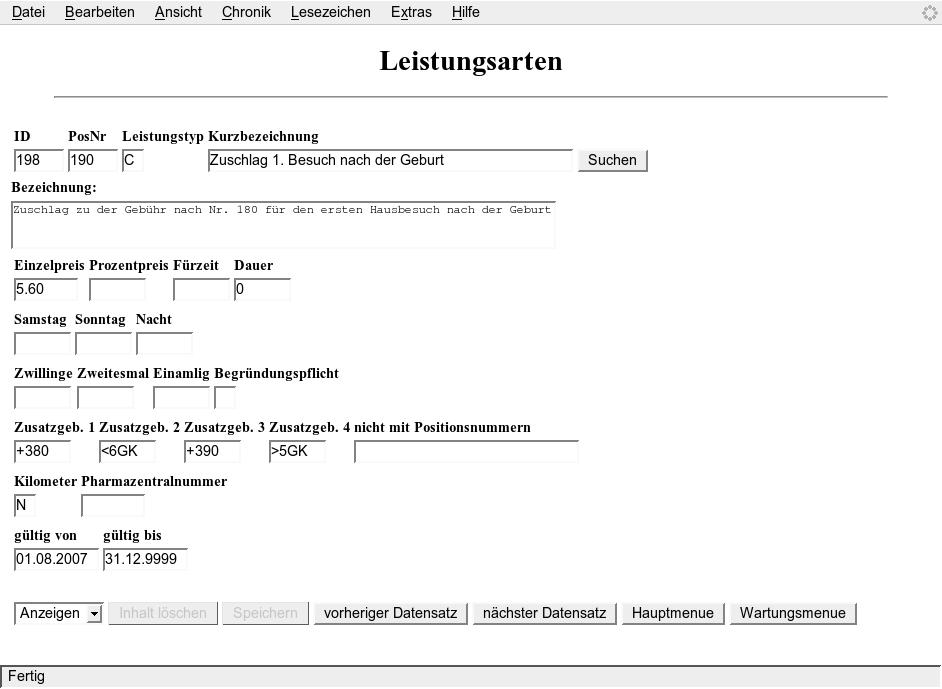
\includegraphics[width=80mm]{leistungsarten}
\caption{Leistungsarten\label{leistungsarten:fig}}
\end{figure}

Folgende Felder sind in der Maske vorhanden:
\begin{description}
\item[ID] Dieses Feld enth�lt die interne ID zum angezeigten Datensatz, das
Feld darf unter keinen Umst�nden ge�ndert oder erfasst werden.
\item[PosNr] Dieses Feld enth�lt die offizielle Positionsnummer der
entsprechenden Leistung gem�� \cite{posnr} oder eine eigene nicht offizielle
Positionsnummer. Eigene Positionsnummern sind sinnvoll f�r Auslagen oder
Materialpauschalen. Es wird empfohlen f�r Materialpauschalen eine fortlaufende
3-stellige Nummer zu vergeben, die mit M beginnt, d.h. M001 bis M999. Der Inhalt
dieses Feldes wird zusammen mit dem Inhalt aus Feld \feld{Kurzbezeichnung}
in der Maske Rechnungsposten erfassen (siehe Abbildung 
\vref{rechnungspostenerfassen:fig}) im Feld \feld{PosNr:} angezeigt.
Analog wird der Inhalt des Feldes zusammen mit der Kurzbezeichnung auf
der Rechnung angedruckt.
\item[Leistungstyp] Dieses Feld enth�lt die Gruppe, der diese 
Leistungsart zugeordnet wird. Es sind f�nf verschiedene Gruppen m�glich:
\begin{enumerate}
\item[A] Mutterschaftsvorsorge,
\item[B] Geburt,
\item[C] Wochenbett,
\item[D] sonstige Leistungen,
\item[M] 
\index{Material}
Material, in Kombination mit dem Feld \feld{Zusatzgeb. 1} wird
entschieden, zu welcher Wirkstoffgruppe diese Materialie geh�rt. D.h. es
ist ein Wert zwischen 500 und 620 nach Hebammen-Verg�tungsverordnung,
bzw. 76 und 88 nach HebGO zu erfassen. Wird im Feld \feld{Zusatzgeb. 1}
nichts erfasst, wird ``sonstige Auslagen (Positionsnummer 70 bzw. 800)'' 
angenommen.
\item[W] 
Wegegeld
\end{enumerate}

Anhand des Leistungstypes werden Plausibilit�tenpr�fungen in der
Rechnungserfassung durchgef�hrt, so sind Leistungen vom Typ A nur bis
zur Geburt des Kindes m�glich und Leistungen vom Typ C nur ab der Geburt
des Kindes.

In der sp�teren Rechnung wird die erfasste Leistung entsprechend ihres
Leistungstypes in der jeweiligen Rubrik in der Rechnung angedruckt.

\item[Kurzbezeichnung] Dieses Feld enth�lt die Kurzbezeichnung der Leistung,
Diese Bezeichnung wird in der Maske Rechnungsposten erfassen im Feld
\feld{PosNr} und auf der sp�teren Rechnung angezeigt. Falls der
Leistungstyp ``M'' ist, wird diese Bezeichnung in die elektronische 
Rechnung �bernommen\footnote{Entweder in Positionsnummer 800, bzw. 70, 
dies sind die einzigen
Positionsnummern, die unterschiedliche Bezeichnungen haben k�nnen.}.
\item[Bezeichnung] Dieses Feld enth�lt die ausf�hrliche Beschreibung der
Leistungsart und wird in der weiteren Anwendung nicht genutzt.
\item[Einzelpreis] Dieses Feld enth�lt den Einzelpreis der Leistungsart.
Dieser Preis wird in der sp�teren Rechnung angedruckt und erscheint in
der �bersicht der erfassten Rechnungsposten in der Maske Rechnungserfassung.
Handelt es sich bei der Leistungsart um eine Leistung die nach Zeit (siehe
Feld \feld{F�rzeit}
abgerechnet wird, wird mit dem Wert aus diesem Feld multipliziert.
Falls die Leistung nur prozentual in Abh�ngigkeit einer anderen Leistung
berechnet werden soll, ist dieses Feld mit Null, resp. nicht zu bef�llen.
Es ist zu beachten, dass in diesem Feld Dezimalstellen mit . (Punkt) und
nicht mit , (Komma) erfasst werden m�ssen, z.B.136.10 und nicht 136,10.
\item[Prozentpreis] Hier einen Wert einzutragen macht nur Sinn, wenn diese
Leistung in Abh�ngigkeit einer anderen Positionsnummer berechnet werden soll.
Ein Beispiel daf�r ist Positionsnummer 18, bei der 25\% Zuschlag 
gerechnet werden m�ssen. Das Feld muss
f�r einen solchen Fall mit 0.25 gef�llt werden.
\item[F�rzeit] �ber dieses Feld wird in der Anwendung gesteuert, ob eine
Leistungsart in Abh�ngigkeit der Zeit berechnet werden muss. In dieses
Feld ist die Zeit in Minuten einzutragen, f�r die jeweils abgerechnet wird.
Wird nur eine Zeit, z.B. 30 eingetragen, bedeutet dies, die Leistungsart
wird pro angefangene Zeit berechnet.
Z.B. bei Positionsnummer 4 ``Hilfe bei Beschwerden'' ist hier 30 
einzutragen, da jede angefangene halbe Stunde abgerechnet werden kann.
Muss die Leistungsart exakt abgerechnet werden, ist ein E vor der Minutenzahl
zu erfassen, z.B. E60. Dies ist z.B. bei Positionsnummer 8 der Fall, d.h.
die Position wird exakt auf 60 Minuten abgerechnet. In diesem Fall werden
auf der Rechnung die Minuten in Stunden umgerechnet und beides angedruckt.
Ist im Feld \feld{F�rzeit} ein Wert gr��er Null erfasst, werden bei Auswahl
der Positionsnummer in der Maske Rechnungserfassung die Felder
\feld{Uhrzeit von} und \feld{Uhrzeit bis} bis f�r die Erfassung freigeschaltet.
\item[Dauer] 
Dieses Feld sollte nur in Kombination mit dem \feld{F�rzeit}
erfasst werden. Ist der Wert gepflegt, wird in der Maske Rechnungserfassung
eine zus�tzliche Plausipr�fung aktiv. Der dort erfasste Zeitraum
(Feld \feld{Uhrzeit bis} Minus Feld \feld{Uhrzeit von}) wird mit der hier 
angegebene Dauer verglichen, ist er gr��er, muss
eine Begr�ndung im Feld \feld{Begr�ndung} erfasst werden.
\item[Samstag] 
In diesem Feld kann auf eine andere Positionsnummer verwiesen
werden. Es wird in der Rechnungserfassung evaluiert, ob das Datum
der Leistungserbringung auf einen Samstag f�llt\footnote{Samstag ist im
Sinne der Hebammengeb�hrenordnung erst nach 12:00, dies wird ber�cksichtigt}.
Wenn dies der Fall ist und im Feld
\feld{Samstag} ein Wert gr��er Null enthalten ist, 
wird die erfasste Positionsnummer
durch die Positionsnummer im Feld \feld{Samstag} ersetzt. Positionsnummer 4
ist ein Beispiel f�r den beschriebenen Sachverhalt. 
Dem Nutzer wird die Substitution durch einen Hinweis angezeigt. 
Wird im Feld
\feld{Samstag} eine Positionsnummer mit einem f�hrenden + (Plus) erfasst,
erfolgt keine Substituierung der Positionsnummer, statt dessen wird die
angegebene Positionsnummer zus�tzlich ausgew�hlt. Positionsnummer 18 ist
ein Beispiel f�r den beschriebenen Sachverhalt. Dem Nutzer wird die
Subsitution durch einen Hinweis angezeigt.
\item[Sonntag] 
F�r das Feld \feld{Sonntag} gilt eine analoge Beschreibung,
wie f�r das Feld \feld{Samstag}. Sonntag und Feiertag werden identisch
behandelt. Die Feiertage m�ssen allerdings zuvor in der Maske Feiertage
erfasst worden sein (siehe dazu \vref{feiertage:abs}).
\item[Nacht] 
F�r das Feld \feld{Nacht} gilt eine analoge Beschreibung,
wie f�r die Felder \feld{Samstag} und \feld{Sonntag}. Nacht ist im Sinne
der Hebammengeb�hrenordung zwischen 20:00 Uhr Abends und 08:00 Uhr Morgens.
\item[Zwillinge] 
Dieses Feld hat in der aktuellen Version keine Bedeutung. Es
ist daf�r vorgesehen die Positionsnummer f�r  Zuschlag Zwillinge aufzunehmen.
Damit dieser Zuschlag automatisch in der Rechnungserfassung ber�cksichtigt
werden kann.
\item[Zweitesmal]
In diesem Feld kann auf eine andere Positionsnummer verwiesen
werden. Es wird in der Rechnungserfassung evaluiert, ob auf eine andere
Positionsnummer verwiesen wird.
Wenn dies der Fall ist und im Feld
\feld{Zweitesmal} ein Wert gr��er Null enthalten ist, 
wird die erfasste Positionsnummer
durch die Positionsnummer im Feld \feld{Zweitesmal} ersetzt. Positionsnummer 22
ist ein Beispiel f�r den beschriebenen Sachverhalt. 
Dem Nutzer wird die Substitution durch einen Hinweis angezeigt. 
\item[Einmalig]
In diesem Feld kann auf eine andere Positionsnummer verwiesen
werden. Es wird in der Rechnungserfassung evaluiert, ob auf eine andere
Positionsnummer verwiesen wird. Wenn dies der Fall ist und im Feld
\feld{Einmalig} eine Positionsnummer mit einem f�hrenden + (Plus) erfasst,
wird die
angegebene Positionsnummer zus�tzlich ausgew�hlt. Positionsnummer 22 ist
ein Beispiel f�r den beschriebenen Sachverhalt. Dem Nutzer wird die
Subsitution durch einen Hinweis angezeigt.
Wird die Positionsnummer ohne f�hrendes Plus erfasst, wird die im Feld
\feld{Posnr} angegebene Positionsnummer ersetzt.
ersetzt.
\item[Begr�ndungspflicht]
Falls in diesem Feld J angegeben ist, wird im Rahmen der Rechnungserfassung
evaluiert, ob eine Begr�ndung erfasst wurde. Ist dies nicht der Fall,
wird dies mit einem Fehlerhinweis angezeigt und die Positionsnummer kann
nicht gespeichert werden. Positionsnummer 8 ist ein Beispiel f�r den
beschriebenen Sachverhalt.
\item[Zusatzgeb.1] 
�ber das Feld \feld{Zusatzgeb.1} werden in Abh�ngigkeit des Leistungstyps
verschiedene Sachverhalte gesteuert.
\begin{enumerate}
\item{Leistungstyp ist M}\\
Falls es sich um Leistungstyp M (Material) handelt, kann �ber das Feld
\feld{Zusatzgeb.1} auf eine Wirkstoffgruppe verwiesen 
werden\footnote{Wird das
Feld nicht erfasst bei Leistungstyp M, wird Positionsnummer 70 (alte
Geb�hrenordnung), bzw. 800 (Hebammen-Verg�tungsvereinbarung)
``sonstige Auslagen'' angenommen.}.
\item{Leistungstyp ist nicht M (Material) und Feld \feld{Zusatzgeb.2} ist leer}\\
Es wird im Rahmen der Rechnungserfassung gepr�ft, ob auf eine 
Materialie verwiesen wird. Ist dies der Fall und das Feld 
\feld{Zusatzgeb.1} ist mit einem f�hrenden + (Plus) erfasst, wird diese
Positionsnummer zus�tzlich ausgew�hlt.\\
Positionsnummer 2 ist ein Beispiel
f�r diesen Sachverhalt, es wird bei Positionsnummer 2 immer zus�tzlich die
entsprechende Materialpauschale (Positionsnummer 71) angew�hlt.
\item{Leistungstyp ist nicht M (Material) und \feld{Zusatzgeb.2} ist nicht leer}\\
Die im Feld \feld{Zusatzgeb.1} angegebene Positionsnummer wird 
zus�tzlich ausgew�hlt, wenn die Bedingung aus dem Feld \feld{Zusatzgeb.2}
erf�llt ist.\\
Positionsnummer 24 ist ein Beispiel f�r diesen Sachverhalt.
\end{enumerate}

\item[Zusatzgeb.2]
In diesem Feld, kann eine zus�tzliche Bedingung zu dem Feld \feld{Zusatzgeb.1}
angegeben werden. Das Feld muss wie folgt erfasst werden:\\
\verb|{Operator}{Zahl}{Vergleichswert}| dabei darf der Operator aktuell nur
die Werte > (gr��er), < (kleiner) oder = (gleich) enthalten. Die Zahl darf
nur Werte zwischen 0 und 999 enthalten. Als Vergleichswert ist aktuell nur 
der Wert GK (Geburtsdatum Kind) vorgesehen.
\paragraph{Beispiel}
Bei Positionsnummer 24 handelt es sich um den Zuschlag 1. Besuch nach der
Geburt. Wenn dies der Fall ist, kann auch die entsprechende Materialpauschale
Positionsnummer 74 oder 75 gew�hlt werden. D.h. bedeutet, in Feld
\feld{Zusatzgeb.1} wird +75 erfasst, die Bedingung in Feld 
\feld{Zusatzgeb.2} >4GK, d.h. liegt der Tag des ersten Besuches mehr als vier
Tage nach der Geburt des Kindes, wird Positionsnummer 75 zus�tzlich ausgew�hlt.
\item[Zusatzgeb.3]
Dieses Feld hat eine �hnliche Beschreibung wie Feld \feld{Zusatzgeb.1}, es
wird allerdings nur in Kombination mit Feld \feld{Zusatzgeb.4} genutzt.
Die hier angegeben Positionsnummer wird ausgew�hlt, wenn die Bedingung aus
Feld \feld{Zusatzgeb.4} erf�llt ist.
\item[Zusatzgeb.4]
In diesem Feld kann eine zus�tzliche Bedingung zu dem Feld \feld{Zusatzgeb.3}
angegeben werden. Das Feld muss wie folgt erfasst werden:\\
\verb|{Operator}{Zahl}{Vergleichswert}| dabei darf der Operator aktuell nur
die Werte > (gr��er), < (kleiner) oder = (gleich) enthalten. Die Zahl darf
nur Werte zwischen 0 und 999 enthalten. Als Vergleichswert ist aktuell nur 
der Wert GK (Geburtsdatum Kind) vorgesehen.
\paragraph{Beispiel}
Bei Positionsnummer 24 handelt es sich um den Zuschlag 1. Besuch nach der
Geburt. Wenn dies der Fall ist, kann auch die entsprechende Materialpauschale
Positionsnummer 74 oder 75 gew�hlt werden. D.h. bedeutet, in Feld
\feld{Zusatzgeb.3} wird +74 erfasst, die Bedingung in Feld 
\feld{Zusatzgeb.4} <5GK, d.h. liegt der Tag des ersten Besuches weniger
als f�nf
Tage nach der Geburt des Kindes, wird Positionsnummer 74 zus�tzlich ausgew�hlt.
\item[nicht mit Positionsnummer]
In diesem Feld kann eine durch ``,'' Komma separierte Liste von
Positionsnummern angegeben werden, die nicht mit der aktuellen Positionsnummer
an einem Tag erfasst werden d�rfen. Z.B. Positionsnummer 030 darf nicht mit
den Positionsnummern 010, 030 am gleichen Tag erfasst werden.
\item[Kilometer]
�ber dieses Feld wird gesteuert, ob in der Maske Rechnungsposten erfassen,
die Felder \feld{Kilometer Tag} und \feld{Kilometer Nacht} f�r die Erfassung
freigeschaltet sind. Durch Eingabe von ``J'' werden die Felder freigeschaltet,
durch die Eingabe von ``N'' f�r die Erfassung gesperrt.
\item[Pharmazentralnummer]
\index{PZN|see{Pharmazentralnummer}}
\index{Pharmazentralnummer}
In diesem Feld muss die Pharmazentralnummer (PZN) bei Materialien angegeben
werden\footnote{ab 01.02.2008 ist es Pflicht die Pharmazentralnummer bei 
elektronischen Rechnungen zu �bermitteln}. Diese Nummer ist auf den
Medikamentenpackungen aufgedruckt oder kann in der Apotheke erfragt werden.
\item[g�ltig von]
Dieses Feld gibt an, ab wann die Positionsnummer mit dieser Auspr�gung 
g�ltig ist. Dies ist z.B. sinnvoll, wenn eine neue Geb�hrenordnung ab
einem bestimmten Zeitpunkt gilt. Eine Positionsnummer kann in der Maske
Rechnungsposten erfassen nur dann ausgew�hlt werden, wenn das aktuelle
Tagesdatum gr��er oder gleich dem Feld \feld{g�ltig von} ist und kleiner
oder gleich dem Feld \feld{g�ltig bis}.
\item[g�ltig bis]
Dieses Feld gibt an, bis wann die Positionsnummer mit dieser Auspr�gung 
g�ltig ist. Dies ist z.B. sinnvoll, wenn eine alte Geb�hrenordnung nur
bis zu einem bestimmten Zeitpunkt gilt.
\end{description}


\subsection{Beschreibung der Kn�pfe im Leistungsartenmenue}
\begin{description}
\item[Suchen] Mit dem Knopf \knopf{Suchen} kann eine weitere Maske ge�ffnet
werden, �ber die Leistungsarten gesucht werden k�nnen. Die Beschreibung zu der
Suchmaske befindet sich in Abschnitt \vref{leistungsartensuchen:abs}.
In diese Maske wird der Wert aus dem Feld \feld{Posnr} �bernommen 
und die Suche unmittelbar gestartet.
\item[Inhalt l�schen] Der Knopf \knopf{Inhalt l�schen} ist nur dann
Aktiv, wenn in dem
Pop Down Menue vor dem Knopf der Wert Neu ausgew�hlt wurde. Wird der Knopf
gedr�ckt, werden alle Felder der Maske auf ihren inital Wert gesetzt und das
Pop Down Menue springt auf den Wert Anzeigen,
\item[Speichern/ L�schen] Der Knopf \knopf{Speichern} ist nur dann Aktiv,
wenn im Auswahlmenue entweder der Wert ``Neu'' oder ``�ndern'' gew�hlt wird. 
\par
Falls Neu 
ausgew�hlt wurde, wird eine neue Leistungsart in der Datenbank gespeichert
und das Pop Down Menue springt auf den Wert Anzeigen. Es finden die
identischen Plausipr�fungen, die schon bei den einzelnen Feldern
beschrieben wurden, statt.
\par
Falls �ndern gew�hlt wurde, wird der Datensatz, der sich in der Datenbank
befindet mit den angezeigten Werten �berschrieben und das Pop Down Menue
springt auf den Wert Anzeigen. 
Es finden die
identischen Plausipr�fungen, die schon bei den einzelnen Feldern
beschrieben wurden,
statt.\par
Falls im Pop Down Menue L�schen ausgew�hlt wurde, erh�lt der Knopf die
Beschriftung L�schen. Durch Dr�cken des Knopfes wird der Datensatz aus der
Datenbank gel�scht. Es findet keine Plausipr�fung statt.
Wurde der Datensatz erfolgreich gel�scht, werden
alle Felder der Maske auf ihren Initial-Wert gesetzt und das Auswahlmenue
steht auf den Wert Anzeigen.
\item[vorheriger Datensatz] Dieser Knopf ist nur dann aktiv, wenn der Wert
des Pop Down Menues auf Anzeigen steht. Durch Dr�cken des Knopfes wird auf
den vorherigen Datensatz in der Datenbank gesprungen. Der vorherige Datensatz
ist derjenige mit der n�chst kleineren Positionsnummer, 
als der aktuell angezeigte. Ist
man am ersten Datensatz angekommen, bleibt dieser in der Maske erhalten.
\item[n�chster Datensatz] Dieser Knopf ist nur dann aktiv, wenn der Wert
des Pop Down Menues auf Anzeigen steht. Durch Dr�cken des Knopfes wird auf
den n�chsten Datensatz in der Datenbank gesprungen. Der n�chste Datensatz
ist derjenige mit der n�chst h�heren Positinsnummer, 
als der aktuell angezeigte. Ist
man am letzten Datensatz angekommen, bleibt dieser in der Maske erhalten.
\item[Hauptmenue] �ber diesen Knopf gelangt man in die Maske Hauptmenue.
Dabei ist zu beachten, dass nicht �berpr�ft wird, ob �nderungen oder neu
erfasste Daten gespeichert wurden. Es wird sofort in die Maske Hauptmenue
gesprungen.
\end{description}

Sind alle Felder erfasst, k�nnen die Daten gespeichert werden. Dazu ist
es notwendig im Pop Down Menue unten links den Wert 'Neu' auszuw�hlen.
Sobald dies geschehen ist, wird der Knopf \knopf{Speichern} aktiv 
geschaltet. Dr�ckt man jetzt den Knopf \knopf{Speichern} werden die Daten
zu der Leistungsart permanent abgelegt. Nach dem Speichern wird die Auswahl im 
Pop Down Menue unten links auf den Wert 'Anzeigen' gesetzt.


\section{Leistungsarten suchen\label{leistungsartensuchen:abs}}
In diesem Absatz ist beschrieben, wie Leistungsarten im Datenbestand 
gesucht und ausgew�hlt werden k�nnen. Der  Aufruf erfolgt aus der 
Maske Leistungsarten (siehe Seite \pageref{leistungsarten:fig}) 
�ber den Knopf \knopf{Suchen}. 
Klickt man auf den Knopf \knopf{Suchen} wird ein neues Fenster mit der
�berschrift ``Leistungsarten suchen'' ge�ffnet\footnote{sollte das Fenster 
noch ge�ffnet sein, wird es in den Vordergrund des Bildschirms geholt.} 
(siehe Abbildung \vref{leistungsartensuchen:fig}). �ber die Felder \feld{Posnr,
Kurzbezeichnung, G�ltigkeit, Leistungstyp} ist es m�glich 
Suchkriterien vorzugeben, d.h. es werden bei der Suche nur die Leistungsarten
ausgegeben, bei denen alle vorgegebenen Werte vorhanden sind. Dabei ist
folgendes f�r die Felder zu beachten:

\begin{figure}[ht]
\centering
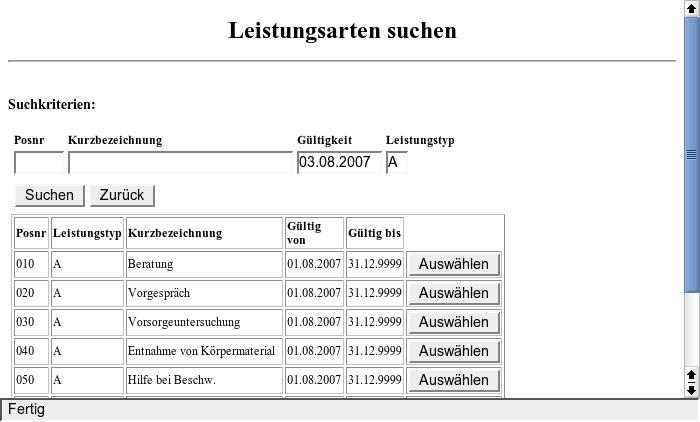
\includegraphics[width=9cm]{leistungsartensuchen}
\caption{Leistungsarten suchen\label{leistungsartensuchen:fig}}
\end{figure}

\begin{description}
\item[Posnr] 
Es wird nur nach den Leistungsarten gesucht, bei denen die Positionsnummer
exakt dem Feldes entspricht.
\item[Kurzbezeichnung] 
Es wird nur nach den Leistungsarten gesucht, bei denen die
Beschreibung mit dem Feldinhalt beginnt. Wird z.B. im Feld 
\feld{Kurzbezeichnung} ``Tel'' erfasst,
w�rden alle Leistungsarten, bei denen die Kurzbezeichnung mit ``Tel'' beginnt 
ermittelt werden, d.h. ``Telefon. Beratung im W.-Bett'' und ``Tel. Beratung
bei Stillschwierigk.''
\item[G�ltigkeit]
Es wird nach den Leistungsarten gesucht, bei denen der Wert ``g�ltig von''
kleiner ist als der im Feld \feld{G�ltigkeit}  erfasste Wert und
``g�ltig bis'' gr��er ist als der im Feld \feld{G�ltigkeit} erfasste Wert.
Wird dieses Feld leer gelassen, wird automatisch mit dem Tagesdatum gesucht.
Um unabh�ngig vom Datum zu suchen, kann '*' oder '\%' erfasst werden.
In der Regel sollte man den Wert leer lassen.

\item[Leistungstyp] 
Es wird nur nach den Leistungsarten gesucht, bei denen der Leistungstyp
exakt der Vorgabe entspricht. D.h. wird hier ein ``C'' erfasst,
werden ausschlie�lich Positionsnummern aus dem Bereich Wochenbett
ermittelt.
\end{description}

Der Werte der Positionsnummer wird aus der Maske Leistungsarten
in die Suchkriterien �bernommen und die Suche gestartet.
Die Felder k�nnen jederzeit mit neuen Kriterien gef�llt und die Suche
�ber den Knopf \knopf{Suchen} gestartet werden.

Das Ergebnis der Suche wird unmittelbar unter den Suchkriterien ausgegeben.
Es werden die Daten zu Positionsnummer, Leistungstyp, Kurzbezeichnung und
der G�ltigkeitszeitraum ausgegeben.

�ber den Knopf \knopf{Ausw�hlen} werden die Daten der Leistungsart in die Maske
�bernommen, aus der die Suchfunktion aufgerufen wurde. Die Maske
``Leistungsarten suchen''
wird danach geschlossen.

Falls keine Leistungsart den gew�nschten Suchkriterien entspricht, 
kann entweder
durch Klicken des Knopfes \knopf{Zur�ck} die Maske ``Leistungsarten suchen''
geschlossen werden, oder es k�nnen andere Suchkriterien erfasst werden.




\section{Feiertage\label{feiertage:abs}}
\index{Feiertage}
Wie schon im Kapitel Installation beschrieben, geh�ren auch die Feiertage
im weitesten Sinne zu den Parametern, da �ber die Feiertage gesteuert
wird, ob an diesen Tagen Zuschl�ge berechnet, beziehungsweise bestimmte
Positionsnummern zu erfassen sind.
Aus dem Hauptmenue gelangt man �ber den Link \nolinkurl{Feiertage}
in die Maske Feiertage (Abbildung \vref{feiertage:fig}).

\begin{figure}[ht]
\centering
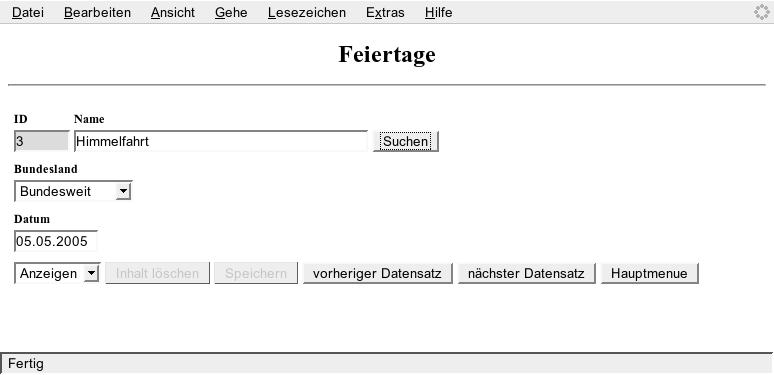
\includegraphics[width=80mm]{feiertage}
\caption{Feiertage\label{feiertage:fig}}
\end{figure}

Folgende Felder sind in der Maske vorhanden:
\begin{description}
\item[ID] 
Dieses Feld enth�lt die interne ID zum angezeigten Datensatz, es
kann nicht ge�ndert oder erfasst werden.
\item[Name] 
Dieses Feld enth�lt die den Namen des Feiertages, z.B.
1. Weihnachtsfeiertag.
\item[Bundesland] 
Dieses Feld enth�lt das Bundesland in dem der Feiertag
\index{Bundesland}
gilt oder ``Bundesweit'', wenn es sich um einen Bundesweiten Feiertag
handelt. In der aktuellen Version von \tinyHeb\/ wird das Bundesland
bei der Ermittlung des Feiertages -- z.B. in der Rechnungserfassung -- 
nicht ber�cksichtigt\footnote{Dies wird sich in einer sp�teren
Version von \tinyHeb\/ �ndern, schickt mir eine Mail, wenn Ihr die
Anforderung schon jetzt habt.}. D.h. es sollte bis auf weiteres immer
Bundesweit in dem Feld erfasst werden.
\item[Datum] 
Dieses Feld enth�lt das Datum des Feiertages. Die Erfasung muss im Format
TT.MM.JJJJ oder TT.MM.JJ erfolgen. Wird das Datum im Format TT.MM.JJ 
erfasst, erfolgt nach Verlassen des Feldes automatisch die Ermittlung
und Darstellung der 4-stelligen Jahreszahl. Ein ung�ltiges Datum f�hrt
zu der Fehlermeldung: ``Bitte g�ltiges Datum erfassen''. Das Speichern
des Formulares mit ung�ltigen Werten ist nicht m�glich.
\end{description}

\subsection{Beschreibung der Kn�pfe im Feiertagemenue}
\begin{description}
\item[Suchen] Mit dem Knopf \knopf{Suchen} kann eine weitere Maske ge�ffnet
werden, �ber die Feiertage gesucht werden k�nnen. Die Beschreibung zu der
Suchmaske befindet sich in Abschnitt \vref{feiertagsuchen:abs}.
In diese Maske werden die Werte aus den Feldern \feld{Name, Bundesland} sowie
\feld{Datum} �bernommen und die Suche unmittelbar gestartet.
\item[Inhalt l�schen] Der Knopf \knopf{Inhalt l�schen} ist nur dann
Aktiv, wenn in dem
Pop Down Menue vor dem Knopf der Wert ``Neu'' ausgew�hlt wurde. Wird der Knopf
gedr�ckt, werden alle Felder der Maske auf ihren Inital-Wert gesetzt und das
Pop Down Menue springt auf den Wert Anzeigen,
\item[Speichern/ L�schen] Der Knopf \knopf{Speichern} ist nur dann aktiv,
wenn im Auswahlmenue entweder der Wert ``Neu'' oder ``�ndern'' gew�hlt wird. 
\par
Falls ``Neu''
ausgew�hlt wurde, wird ein neuer Feiertag in der Datenbank gespeichert
und das Pop Down Menue springt auf den Wert Anzeigen. Es finden die
identischen Plausipr�fungen, die schon bei den einzelnen Feldern
beschrieben wurden, statt.
\par
Falls ``�ndern'' gew�hlt wurde, wird der Datensatz, der sich in der Datenbank
befindet mit den angezeigten Werten �berschrieben und das Pop Down Menue
springt auf den Wert Anzeigen. 
Es finden die
identischen Plausipr�fungen, die schon bei den einzelnen Feldern
beschrieben wurden,
statt.\par
Falls im Pop Down Menue L�schen ausgew�hlt wurde, erh�lt der Knopf die
Beschriftung L�schen. Durch Dr�cken des Knopfes wird der Datensatz aus der
Datenbank gel�scht. Es findet keine Plausipr�fung statt.
Wurde der Datensatz erfolgreich gel�scht, werden
alle Felder der Maske auf ihren Initial-Wert gesetzt und das Auswahlmenue
steht auf den Wert Anzeigen.
\item[vorheriger Datensatz] Dieser Knopf ist nur dann aktiv, wenn der Wert
des Pop Down Menues auf Anzeigen steht. Durch Dr�cken des Knopfes wird auf
den vorherigen Datensatz in der Datenbank gesprungen. Der vorherige Datensatz
ist derjenige mit der n�chst kleineren ID, als der aktuell angezeigte. Ist
man am ersten Datensatz angekommen, bleibt dieser in der Maske erhalten.
\item[n�chster Datensatz] Dieser Knopf ist nur dann aktiv, wenn der Wert
des Pop Down Menues auf Anzeigen steht. Durch Dr�cken des Knopfes wird auf
den n�chsten Datensatz in der Datenbank gesprungen. Der n�chste Datensatz
ist derjenige mit der n�chst h�heren ID, als der aktuell angezeigte. Ist
man am letzten Datensatz angekommen, bleibt dieser in der Maske erhalten.
\item[Hauptmenue] �ber diesen Knopf gelangt man in die Maske Hauptmenue.
Dabei ist zu beachten, dass nicht �berpr�ft wird, ob �nderungen oder Neu
erfasste Daten gespeichert wurden. Es wird sofort in die Maske Hauptmenue
gesprungen.
\end{description}

Sind alle Felder erfasst, k�nnen die Daten gespeichert werden. Dazu ist
es notwendig im Pop Down Menue unten links den Wert 'Neu' auszuw�hlen.
Sobald dies geschehen ist, wird der Knopf \knopf{Speichern} aktiv 
geschaltet. Dr�ckt man jetzt den Knopf \knopf{Speichern} werden die Daten
zu dem Feiertag permanent abgelegt. Nach dem Speichern wird die Auswahl im 
Pop Down Menue unten links auf den Wert 'Anzeigen' gesetzt.

\section{Feiertag suchen\label{feiertagsuchen:abs}}
In diesem Absatz ist beschrieben, wie Feiertage im Datenbestand gesucht und
ausgew�hlt werden k�nnen. Der  Aufruf erfolgt aus der 
Maske Feiertage (siehe Seite \pageref{feiertage:fig}) 
�ber den Knopf \knopf{Suchen}. 
Klickt man auf den Knopf \knopf{Suchen} wird ein neues Fenster mit der
�berschrift ``Feiertag suchen'' ge�ffnet\footnote{sollte das Fenster 
noch ge�ffnet sein, wird es in den Vordergrund des Bildschirms geholt.} 
(siehe Abbildung \vref{feiertagsuchen:fig}). �ber die Felder \feld{Name,
Bundesland, Datum} ist es m�glich 
Suchkriterien vorzugeben, d.h. es werden bei der Suche nur die Feiertage
ausgegeben, bei denen alle vorgegebenen Werte vorhanden sind. Dabei ist
folgendes f�r die Felder zu beachten:

\begin{figure}[ht]
\centering
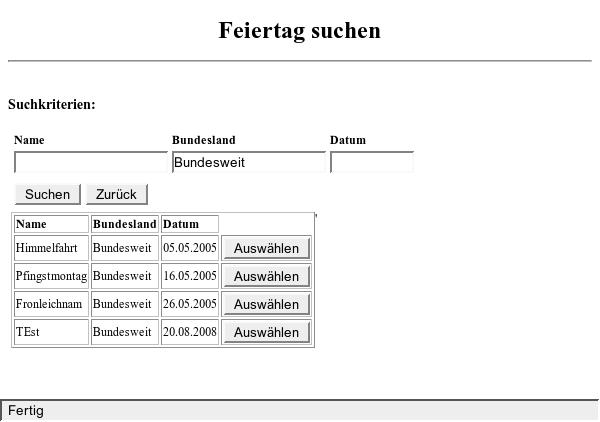
\includegraphics[width=9cm]{feiertagsuchen}
\caption{Feiertag suchen\label{feiertagsuchen:fig}}
\end{figure}

\begin{description}
\item[Name] 
Es wird nur nach den Feiertagen gesucht, bei denen der Name
einen Teil des Feldes enth�lt.
Wird z.B. im Feld \feld{Name} ``Weihn'' erfasst,
w�rde ``1. Weihnachtstag'' und ``2. Weihnachtstag'' ermittelt werden.
\item[Bundesland] 
Es wird nur nach den Feiertagen gesucht, bei denen die
Beschreibung mit dem Feldinhalt beginnt. Wird z.B. im Feld 
\feld{Bundesland} ``B'' erfasst,
w�rden alle Feiertage, bei denen das Bundesland mit ``B'' beginnt 
ermittelt werden, d.h. ``Bayern'' und ``Bundesweit''
\footnote{wobei in der aktuellen Version nur Bundesweit Sinn macht,}.
\item[Datum] Es wird nur nach den Feiertage gesucht, die diesen Wert
enthalten.
\end{description}

Die Werte Name und Bundesland
in die Suchkriterien �bernommen und die Suche gestartet.
Die Felder k�nnen jederzeit mit neuen Kriterien gef�llt und die Suche
�ber den Knopf \knopf{Suchen} gestartet werden.

Das Ergebnis der Suche wird unmittelbar unter den Suchkriterien ausgegeben.
Es werden die Daten zu Name, Bundesland und Datum ausgegeben.

�ber den Knopf \knopf{Ausw�hlen} werden die Daten des Feiertages in die Maske
�bernommen, aus der die Suchfunktion aufgerufen wurde. Die Maske
``Feiertag suchen''
wird danach geschlossen.

Falls keine Feiertage den gew�nschten Suchkriterien entsprichen, kann entweder
durch Klicken des Knopfes \knopf{Zur�ck} die Maske ``Feiertag suchen''
geschlossen werden, oder es k�nnen andere Suchkriterien erfasst werden.


%%% Local Variables: 
%%% mode: latex
%%% TeX-master: t
%%% End: 


% $Id: anhang.tex,v 1.14 2010/08/10 08:17:41 baum Exp $
% Tag $Name: tinyheb-1-6-3 $

% Copyright (C) 2004 - 2009 Thomas Baum <thomas.baum@arcor.de>
% Thomas Baum, 42719 Solingen, Germany

% This program is free software; you can redistribute it and/or modify
% it under the terms of the GNU General Public License as published by
% the Free Software Foundation; either version 2 of the License, or
% (at your option) any later version.

% This program is distributed in the hope that it will be useful,
% but WITHOUT ANY WARRANTY; without even the implied warranty of
% MERCHANTABILITY or FITNESS FOR A PARTICULAR PURPOSE.  See the
% GNU General Public License for more details.

% You should have received a copy of the GNU General Public License
% along with this program; if not, write to the Free Software
% Foundation, Inc., 59 Temple Place - Suite 330, Boston, MA 02111-1307, USA.



\appendix
\chapter{Anhang}

\section{Anmeldung zum E-Mail Verfahren\label{anhang:elekrech}}
\index{Datenaustausch!Anmeldung}
Hier findet sich die Beschreibung, was zu tun ist, um Rechnungen per
E-Mail zu verschicken. Der hier beschriebene Weg ist vom Autor selbst
beschritten worden. Dies wird ausdrücklich erwähnt, weil sich im Internet
an unterschiedlichsten Stellen Anweisungen finden, was zu tun ist und
wie viel es kostet. Diese Beschreibungen sind oft nicht korrekt, insb.
ist es nicht notwendig Geld für eine Zulassung zum Datenaustausch
auszugeben.

Wie immer im Leben führen viele Wege nach Rom und genau so ist es auch
mit der Zulassung zum Datenaustausch. 

\paragraph{Weg 1}
Auf der Anmeldeseite der ITSG \cite{itsg_email_anmeldung} findet sich
seit März 2006 ein Hinweis, dass nach dem Beschluss der Technischen
Arbeitsgruppe eine Anmeldung zum Praxisverfahren für Leistungserbringer
und Arbeitgeber nicht mehr erforderlich ist und aus diesem Grund die
entsprechenden Anmeldeformulare auf dieser Internet-Seite nicht mehr zu
Verfügung stehen.

Das ist auch gut so, weil eine Anmeldung über dieses Formular nicht 
funktionierte. Daher geht man besser Weg 2:

\paragraph{Weg 2}
Dieser Weg führt einen zu den verschiedenen Datenannahmestellen, bzw.
den einzelnen Krankenkassen und den in \cite{datenaustausch302} genannten
Ansprechpartnern. Welche das sind, ist in Tabelle \ref{krankenkassen302}
aufgeführt, unbedingt anmelden muss man sich beim VdAK.

\paragraph{}

\bottomcaption{Krankenkassen und Ansprechpartner\label{krankenkassen302}}
\tablehead
{\hline \bfseries Krankenkassen&\bfseries Anmeldung und Ansprechpartner\\ \hline}

\tabletail
{\hline \multicolumn{2}{r}{\emph{Fortsetzung auf der nächsten Seite}}\\}

\tablelasttail{\hline}
\begin{mpsupertabular}{|p{4cm}|p{9.8cm}|}

Allgemeine Ortskrankenkassen (AOK)&
\index{AOK}
Eine Anmeldung ist bei den AOKen nicht notwendig. Ein Anruf bei dem in
\cite{datenaustausch302} genannten Ansprechpartner ist trotzdem sinnvoll.
\\ \hline
\index{BKK}
\index{ARZ-Emmendingen}
BKK Bundesverband&
Eine Anmeldung beim BKK Bundesverband ist nicht
erforderlich. Da die BKKen i.d.R. über das Abrechnungszentrum Emmendingen
ihre Rechnungen verarbeiten lassen, ist eine Anmeldung dort notwendig.
Diese Anmeldung kann telefonisch erfolgen. Die SEHR freundlichen
Ansprechpartner finden sich im Internet unter 
{\href{http://www.arz-emmendingen.de/daten/daten.php}{\nolinkurl{http://www.arz-emmendingen.de/daten/daten.php}}}. Ansprechpartner für Hebammen ist
Herr Goldschmidt 07641 9201-315. Die Freischaltung zum E-Mail-Verfahren wird
per E-Mail bestätigt. Bitte Herrn Goldschmidt mitteilen, dass ihr
\tinyHeb\/ nutzt, dann werdet ihr schneller zum Echtbetrieb zugelassen.
\\ \hline
\index{DDG}
BKK Bundesverband und IKK (DDG)&
nicht alle BKK's und IKK's
rechnen über das Abrechnungszentrum Emmendingen ab, ein Teil arbeitet 
mit der DDG zusammen. Bei der DDG gibt es ein Online Ameldeformular unter
{\href{http://www-ddg-online.de/dta/formemail.php3}{\nolinkurl{http://www-ddg-online.de/dta/formemail.php3}}}. Sollte die Anmeldung
nicht per E-Mail bestätigt werden, hilft ein Anruf bei Herrn Numratzki
Tel. 0201/8998-980.
\\ \hline
\index{Medent}
\index{Techniker-Krankenkasse}
\index{TKK|see{Techniker-Krankenkasse}}
\index{VdAK}
Ersatzkassen (VdAK/AEV)&
Hier ist eine Anmeldung notwendig, da über den
VdAK die Freischaltung bei der T-Systems erfolgt. Nur durch diese Freischaltung
bei der T-Systems ist es möglich, Rechnungen an den IKK Bundesverband zu
schicken. Das Anmeldeformular für den VdAK steht im Internet zum Download
zur Verfügung {\href{http://www.vdak.de/vertragspartner/sonstige-vertragspartner/Abrechnungsverfahren/index.htm}{\nolinkurl{http://www.vdak.de/vertragspartner/sonstige-vertragspartner/Abrechnungsverfahren/index.htm}}}.
Die Freischaltung wurde per E-Mail
bestätigt. Die Weiterleitung der Anmeldung an die T-Systems erfolgt 
Mittwochs und Freitags. Die Ersatzkassen nutzen unterschiedliche
Datenannahmestellen, nicht bei allen ist eine Anmeldung erforderlich. So
gilt z.B. für die Techniker Krankenkasse, das diese die Medent GmbH als
Datenannahmestelle beauftragt hat. Bei Medent ist keine Anmeldung
erforderlich. Medent nimmt nur verschlüsselte und signierte Rechnungen
entgegen.
\\ \hline

\index{IKK}
IKK Bundesverband&
Hier ist eine Anmeldung notwendig. Diese hilft aber nur
dann weiter, wenn auch die Freischaltung beim VdAK beantragt wurde.
Vermutlich ist sogar eine Anmeldung beim VdAK ausreichend, ich hatte meine
Frau zunächst beim IKK Bundesverband und erst danach beim VdAK
angemeldet. Ansprechpartner beim IKK Bundesverband ist Herr Andreas Kinas
02204/44-491, {\href{email:andreas.kinas@bv.ikk.de}{\nolinkurl{email:andreas.kinas@bv.ikk.de}}}. Die Anmeldung kann per
E-Mail erfolgen, es werden die gleichen Informationen wie schon beim
VdAK benötigt. Die Anmeldung wird schriftlich bestätigt.
\\ \hline

\end{mpsupertabular}



\section{Aktualisierung der Krankenkassendaten\label{anhang:aktkk}}
\index{Krankenkassen!Anschriften}
\index{Kostenträgerdateien}
\subsection{Verarbeitung der Kostenträgerdateien\label{anhang:ktrdat}}
Die Krankenkassendaten, d.h. Name, Anschrift oder Ansprechpartner werden
in den sogenannten Kostenträgerdateien \cite{ktrdat} zur Verfügung gestellt.
Diese Dateien werden von den Spitzenverbänden der einzelnen 
Krankenkassen zum Quartalsende im Internet veröffentlicht.
Sollte es im Laufe eines Quartals nötig sein, Änderungen an den Daten
vorzunehmen, werden auch diese Änderungen veröffentlicht.
Es gibt eine zentrale Adresse im Internet {\href{http://www.gkv-datenaustausch.de/Leistungserbringer_Sole_Kostentraegerdateien.gkvnet}
{\nolinkurl{http://www.gkv-datenaustausch.de/Leistungserbringer_Sole_Kostentraegerdateien.gkvnet}}}
an der die
Dateien heruntergeladen werden können. 
Die Dateien können entweder aus aus der Kommandozeile mit dem Programm
\verb|kostentraeger.pl| aus dem Verzeichnis \verb|tools| eingelesen werden,
oder über die Maske ``Kostenträgerdateien einspielen'', die aus dem 
Wartungsmenue aufgerufen werden kann.

\paragraph{Maske Kostenträgerdateien einspielen}

Die Maske ``Kostenrägerdateien einspielen'' ist in zwei Bereiche geteilt.
Im oberen Teil der Maske lässt sich einstellen, welche Kostenträgerdatei
eingelesen werden soll und ob ein Testlauf oder Update durchgeführt werden
soll.

Der Dateiname der Kostenrägerdatei muss im Feld 
\feld{Dateiname der Kostenträgerdatei} angegeben werden. Über den 
Knopf \knopf{Durchsuchen} kann alternativ ein Dateibrowser geöffnet werden,
über den die Datei ausgewählt werden kann.

Bevor ein Update auf die Datenbank gemacht wird, ist es sinnvoll einen
Testlauf durchzuführen, um zu überprüfen, welche Daten sich geändert haben.
Dazu ist \feld{Testlauf} zu markieren.

Über den Knopf \knopf{Kostenträgerdatei einspielen} kann der Testlauf, resp.
der Update auf die Datenbank gestartet werden. Im Unteren Bereich der Maske
wird angezeigt, bei welchen Krankenkassen es zu Änderungen gekommen ist und
welche Felder im einzelnen geändert wurden.

\begin{figure}[H]
\centering
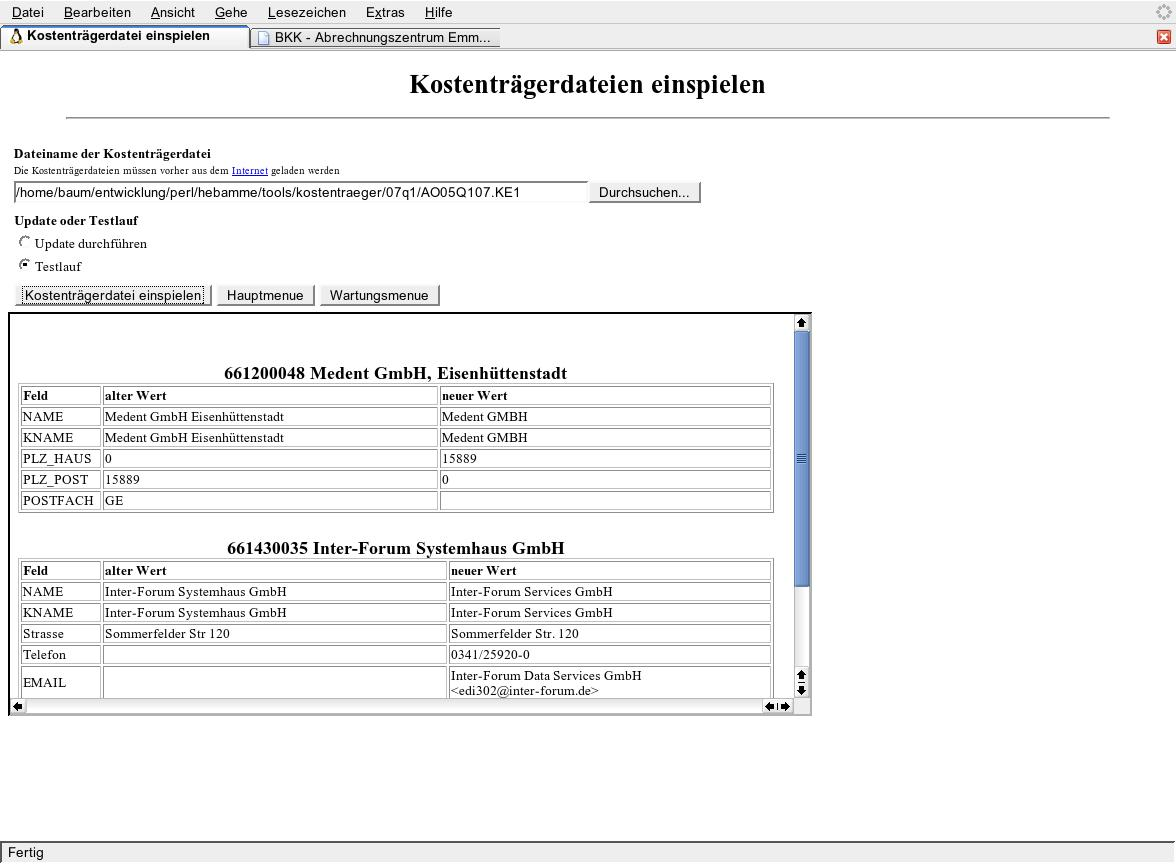
\includegraphics[width=9cm]{kostentraegerdateien}
\caption{Kostenträgerdateien einspielen\label{kostentraegerdateien:fig}}
\end{figure}


\paragraph{Beschreibung des Kommandozeilentools}
\index{kostentraeger.pl}
Mit dem Programm \verb|kostentraeger.pl| im Verzeichnis \verb|tools| können
die Kostenträgerdateien der Krankenkassen
automatisch eingelesen werden. Das Programm muss wie folgt aufgerufen werden:\\
\\
\verb|kostentraeger.pl Optionen|. \\
\\
Folgende Optionen sind möglich:
\begin{compactdesc}
\item\textbf{-h} (Help) gibt eine Bedienungshilfe aus.
\item\textbf{-p} (Pfad) Pfad zu den Kostenträgerdateien.
\item\textbf{-f} (File) die Kostenträgerdatei.
\item\textbf{-o} (Out) der Inhalt der Kostenträgerdatei werden durch TAB \verb|\t| getrennt
ausgegeben. Dadurch ist es möglich Ausgabe in einer Datei zu speichern und
z.B. in einer Tabellenkalkulation weiter zu verarbeiten oder es kann
ein Ladebestand für eine Datenbank generiert werden.
\item\textbf{-c} (Check) Vergleich der Krankenkassen aus der Datenbank mit den Daten aus
der Eingabedatei. Krankenkassen die nicht im Datenbankbestand vorhanden sind,
werden als neue Krankenkassen ausgegeben.
\item\textbf{-n} (New) Ausgabe der Krankenkassen, deren Daten sich zwischen der Eingabedatei
und dem Datenbankbestand unterscheiden, inkl. der Felder, die sich geändert
haben. Nur sinnvoll in Kombination mit Option -c.
\item\textbf{-u} (Update) Geänderte Daten aus der Eingabedatei überschreiben Werte in
der Datenbank. Nur sinnvoll in Kombination mit Option -c.
\item\textbf{-d} (Delete) Es werden die Krankenkassen ausgegeben, die sich in der
Datenbank, aber nicht in der Eingabedatei befinden.
\item\textbf{-v} (Verbose) jede Menge zusätzliche Ausgabem, ist für Debugging sinnvoll.
\end{compactdesc}

\paragraph{Beispiele}
\begin{compactdesc}
\item\textbf{kostentraeger.pl -p kostentraeger/06q2/ -f IK05Q206.KE1 -o}\\
Ausgabe aller Krankenkassen aus der Kostenträgerdatei IK05Q206.KE1 aus 
dem Verzeichnis kostentraeger/06q2/.
\item\textbf{kostentraeger.pl -p kostentraeger/06q2/ -f IK05Q206.KE1 -c}\\
Ausgabe der neuen Krankenkassen aus der Datei IK05Q206.KE1 und Ausgabe, bei 
wie vielen Krankenkassen sich Änderungen, bzw. sich keine Änderungen 
ergeben haben.
\item\textbf{ kostentraeger.pl -p kostentraeger/06q2/ -f IK05Q206.KE1 -c -n}\\
Ausgabe der neuen Krankenkassen und Ausgabe aller geänderten Kassen, inkl.
der Angabe, welche Felder sich geändert haben.
\item\textbf{ kostentraeger.pl -p kostentraeger/06q2/ -f IK05Q206.KE1 -c -n -u}\\
Ausgabe der neuen Krankenkassen und Ausgabe aller geänderten Kassen, inkl.
der Angabe, welche Felder sich geändert haben und update auf die
Datenbank durchführen.
\end{compactdesc}


\subsection{Verarbeitung der öffentlichen Schlüssel der
Datenannahmestellen\label{anhang:pubkey}}
\index{\"offentliche Schlüssel}
\index{Public Keys}
Damit der elektronische Datenaustausch mit den Krankenkassen durchgeführt
werden kann, ist es notwendig die Rechnungsdaten zu verschlüsseln.
Das in \tinyHeb\/ genutzte Verschlüsselungsverfahren ist PKCS\#7\footnote{Wer sich für Details der Verschlüsselungsalgorithmen interessiert, kann diese z.B. in \cite{buchmann} nachlesen. Mathe Leistungskurs oder besser einige Semester Mathematik Studium sind Voraussetzung für die Lektüre.}.
Wesentlicher Bestandteil der Verschlüsselung ist der so genannte public
key der Datenannahmestelle.

Die öffentlichen Schlüssel der Datenannahmestellen stehen im Internet
unter der Adresse 
{\href{ftp://trust.itsg.de/dale/}{\nolinkurl{ftp://trust.itsg.de/dale/}}}
zum Download zur Verfügung. Zwei Dateien sind an dieser Stelle von Interesse:
\begin{enumerate}
\item
\index{gesamt-pkcs.key}
\verb|gesamt-pkcs.key| enthält alle öffentlichen PKCS\#7 Schlüssel, unabhängig,
ob es sich um eine Datenannahmestelle oder eine Hebamme handelt.
\item
\index{annahme-pkcs.key}
\verb|annahme-pkcs.key| enthält die öffentlichen PKCS\#7 Schlüssel der
Datenannahmestellen.
\end{enumerate}
\index{key.pl}
Die Schlüssel aus den Dateien können entweder aus der Kommandozeile 
mit dem Programm  \verb|key.pl| aus dem Verzeichnis \verb|tools| in den
Datenhaushalt von \tinyHeb\/ eingelesen werden, oder über die Maske
``öffentliche Schlüssel der Datenannahmestellen einspielen'', die aus
dem Wartungsmenue aufgerufen werden kann.


\paragraph{Maske öffentliche Schlüssel der Datenannahmestellen
einspielen}
\index{Datenannahmestelle!\"offentlicher Schlüssel}
Die Maske ``öffentliche Schlüssel einspielen'' ist in zwei Bereiche
geteilt. Im oberen Teil der Maske lässt sich einstellen, welche 
Schlüsseldatei eingespielt und ob ein Testlauf oder Update durchgeführt
werden soll.

Der Dateiname der Schlüsseldatei muss im Feld
\feld{Dateiname der Schlüsseldatei} angegeben werden. Über den Knopf
\knopf{Durchsuchen} kann alternativ ein Dateibrowser geöffnet werden,
über den die Datei ausgewählt werden kann.

Bevor ein Update auf die Datenbank gemacht wird, ist es sinnvoll einen
Testlauf durchzuführen, um zu prüfen, welche Daten in der Datei enthalten
sind. Dazu ist \feld{Testlauf} zu markieren. 

Über den Knopf \knopf{Schlüsseldatei einspielen} kann der Testlauf,
resp. das Update auf die Datenbank gestartet werden. Die Verarbeitung
kann je nach Rechneraustattung und welche Datei man gewählt hat, einige
Zeit in Anspruch nehmen. Es sollte solange gewartet werden, bis
im unteren Bereich der Maske keine Ausgabe mehr erfolgt.

Im unteren Bereich der Maske wird angezeigt, welche Informationen in
der eingelesenen Schlüsseldatei vorhanden ist. Als Überschrift wird
bei jedem Zertifikat die IK-Nummer und die Kurzbezeichnung zu dieser
IK-Nummer angezeigt\footnote{natürlich nur dann, wenn diese Information
im Datenhaushalt vorhanden ist.}. Folgende Informationen werden
zusätzlich ausgegeben.

\begin{description}
\item[Seriennummer]
Jedes Zertifikat besitzt eine eindeutige Seriennummer. Diese wird hier
angezeigt.

\item[Organisation]
Organisationsbezeichnung für die das Zertifikat ausgestellt wurde.

\item[Ansprechpartner]
Ansprechpartner für das Zertifikat und ``Inhaber'' des privaten Schlüssels
zu diesem Zertifikat.

\item[Gültig von]
Ab wann kann dieses Zertifikat genutzt werden.

\item[Gültig bis]
Bis wann ist dieses Zertifikat gültig.

\item[Herausgeber]
Wer ist Zertifizierungsstelle für dieses Zertifikat.

\item[Länge des Schlüssels]
Wie lang ist der Schlüssel dieses Zertifikates. Ist die Länge des Schlüssels
kleiner als 2000 Bit, wird die Verarbeitung abgebrochen. Vermutlich wurde
versucht die PEM Version der Schlüsseldatei einzulesen. Bei der PEM Version
wird mit Schlüssellängen von 768 Bit gearbeitet.

\item[Algorithmus des Schlüssels]
Mit welchem Verfahren wurde der Schlüssel erzeugt. Hier sollte b.a.w. immer
rsaEncryption stehen.

\item[Status Datenaustausch]
Hier wird angezeigt, ob es sich bei dem Schlüssel dieser Organisation
um eine Datenannahmestelle
handelt oder nicht. Falls es sich um eine Datenannahmestelle handelt, wird
der Schlüssel eingelesen und der Status des Datenaustausches, wie er in
\tinyHeb\/ parametrisiert ist, angezeigt.

\end{description}

\begin{figure}[H]
\centering
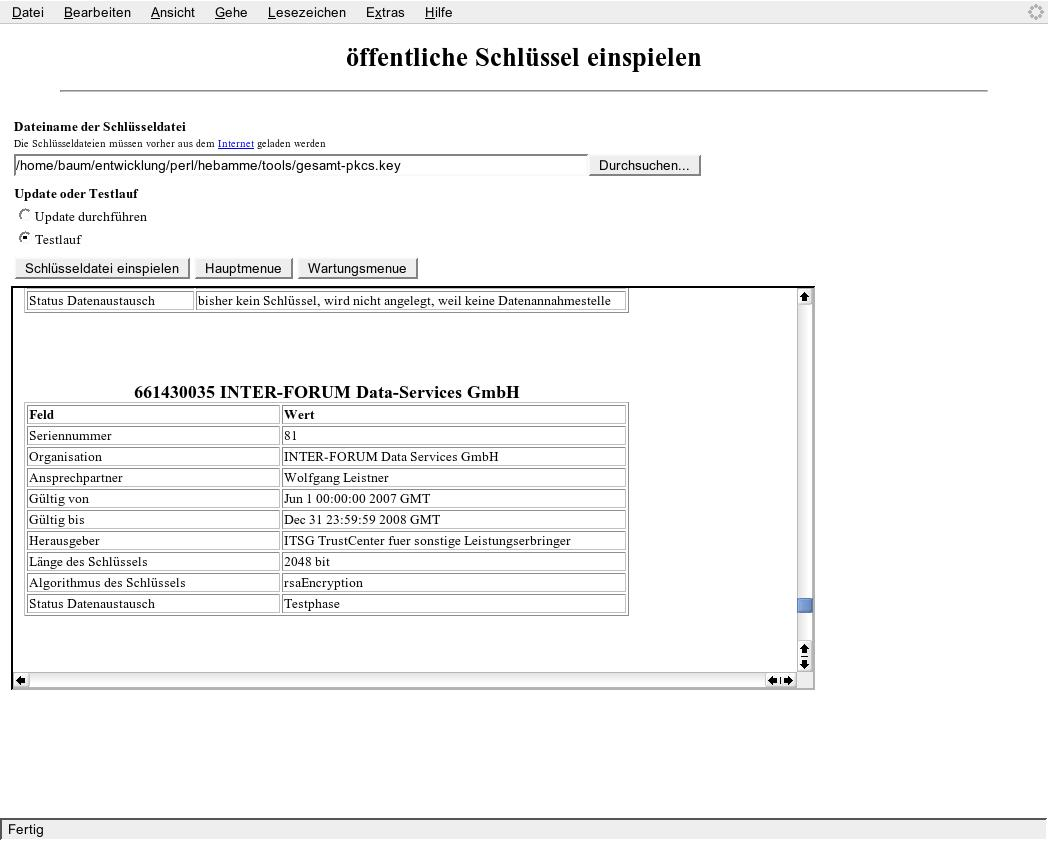
\includegraphics[width=9cm]{schluesseldateien}
\caption{Schlüsseldateien einspielen\label{schluesseldateien:fig}}
\end{figure}


\paragraph{Beschreibung des Kommandozeilen Tools}
Mit dem Programm \verb|key.pl| im Verzeichnis \verb|tools| können die
Schlüsseldateien der Datenannahmestellen automatisch eingelesen werden.
Das Programm muss wie folgt aufgerufen werden:\\
\\
\verb|key.pl| Optionen.\\
\\
Folgende Optionen sind möglich:
\begin{compactdesc}
\item
\textbf{-h} (Help) gibt eine Bedienungshilfe aus.
\item
\textbf{-p} (Pfad) Pfad zu der Schlüsseldatei, kann auch entfallen, wenn sich
die Schlüsseldatei im Verzeichnis \verb|tools| befindet.
\item
\textbf{-f} (File) Name der Schlüsseldatei.
\item
\textbf{-s} (Save) speichert die einzelnen Zertifikate in jeweils 
eigener Datei.
Die generierten Dateinamen lauten IK-Nummer.pem. So kann man zum Beispiel sein
eigenes Zertifikat aus der Datei \verb|gesamt-pkcs.key| extrahieren.
\item
\textbf{-o} (Out) In welches Verzeichnis sollen die einzelnen öffentlichen
Schlüssel der Datenannahmestellen geschrieben werden. Wird dieser Parameter
nicht gesetzt, wird automatisch das Verzeichnis \verb|keys| genutzt. Das
Verzeichnis zum Schreiben der einzelnen Schlüssel muss vorhanden sein.
\item
\textbf{-u} (Update) vorhandene Daten aus der Eingabedatei überschreiben Werte
 in der Datenbank.
\item
\textbf{-v} (Verbose) jede Menge zusätzliche Ausgabem, ist für Debugging 
sinnvoll oder wenn man überprüfen möchte, ob neue Schlüssel dazu gekommen
sind.
\item
\textbf{-c} kopiert das Zertifikat der Hebamme an die richtige Stelle für
die weitere Verarbeitung. Siehe auch Seite \pageref{anhang:eigenes_cert}.
\item
\textbf{-t} (hTml) es wird HTML formatierte Ausgabe generiert.
\end{compactdesc}


\paragraph{Beispiele}
\begin{compactdesc}
\item
\textbf{key.pl -s -f annahme-pkcs.key}\\
Gibt Informationen zu den in der Datei \verb|annahme-pkcs.key| enthaltenen
Schlüsseln aus. Alle einzelnen Schlüssel werden im Verzeichnis keys mit
dem Dateinahmen ik-nummer.pem gespeichert.
\item
\textbf{key.pl -v -s -f gesamt-pkcs.key}\\
Gibt Informationen zu den in der Datei \verb|gesamt-pkcs.key| enthaltenen
Schlüsseln aus. Zusätzlich wird der Gültigkeitszeitraum des Zertifikates
ausgegeben. Alle einzelnen Schlüssel werden im Verzeichnis keys mit
dem Dateinahmen ik-nummer.pem gespeichert.
Diesen Befehl solltet Ihr mal ausprobieren und die Ausgabe nach Hebamme
durchsuchen, dann bekommt Ihr einen Eindruck wie viele Hebammen über ein
PKCS\#7 Zertifikat verfügen.
\item
\textbf{key.pl -s -f annahme-pkcs.key -o annahme}\\
Gibt Informationen zu den in der Datei \verb|annahme-pkcs.key| enthaltenen
Schlüsseln aus. Alle einzelnen Schlüssel werden im Verzeichnis \verb|annahme|
 mit dem Dateinahmen ik-nummer.pem gespeichert.
\item
\textbf{key.pl -s -f annahme-pkcs.key -o annahme -u}\\
Gibt Informationen zu den in der Datei \verb|annahme-pkcs.key| enthaltenen
Schlüsseln aus. Alle einzelnen Schlüssel werden im Verzeichnis \verb|annahme|
 mit dem Dateinahmen ik-nummer.pem gespeichert. Zusätzlich werden die
Schlüssel in den \tinyHeb\/ Datenhaushalt übernommen. 
\end{compactdesc}


\section{zusätzliche Provider im elektronischen Datenaustausch\label{anhang:provider}}
Im Rahmen des elektronischen Datenaustausches ist es ggf. notwendig
unterschiedliche E-Mail Provider für den Datenaustausch zu nutzen, insb.
weil das ARZ-Emmendingen in der Regel keine E-Mails vom Provider Arcor
akzeptiert.
Es gibt zwei Möglichkeiten die notwendigen Informationen zu hinterlegen.
Entweder durch Editieren der Datei \verb|.xauftragrc| oder
seit \tinyHeb\/ Version 1.1.0 aus der Anwendung \verb|xauftrag.pl|.

\paragraph{Aus der Anwendung xauftrag.pl}

\begin{figure}[ht]
\centering
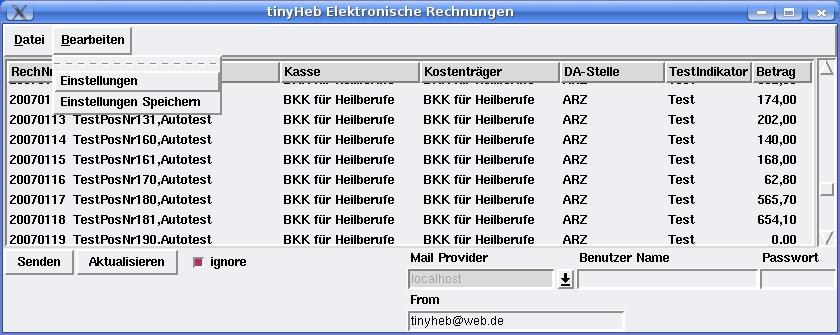
\includegraphics[width=80mm]{xauftrag_bearbeiten}
\caption{Elektronische Rechnungen, Maileinstellungen \label{anhang:xauftrag:fig}}
\end{figure}

Dazu ist zunächst die Anwendung \verb|xauftrag.pl| aus dem Verzeichnis
\verb|edifact| zu starten -- siehe dazu auch Kapitel \vref{elekrechnung:kap} 
und Abbildung \vref{anhang:xauftrag:fig}.


Durch Klicken auf Bearbeiten und Einstellungen öffnet sich ein neues 
Fenster (Abbildung \vref{anhang:xauftrag_einstellungen:fig}), 
in dem  Angaben bzgl. der 
einzelnen Provider, bzw. der einzelnen Mail Accounts geändert werden können.

Hat man die Angaben geändert muss der Knopf 
\knopf{Einstellungen übernehmen und Schließen} gedrückt werden, damit die
Änderungen in die laufende Anwendung übernommen werden. Das Fenster schließt
sich nachdem der Knopf gedrückt wurde.
So kann man z.B. zunächst Testen, ob die Änderungen den gewünschten Effekt 
haben. Sollen die Angaben permanent verfügbar sein, muss der Knopf
\knopf{Einstellungen Speichern} aus Abbildung \vref {anhang:xauftrag:fig}
gedrückt werden.

\begin{figure}[ht]
\centering
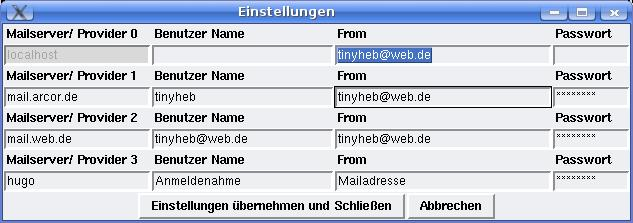
\includegraphics[width=80mm]{xauftrag_einstellungen}
\caption{Elektronische Rechnungen, Maileinstellungen \label{anhang:xauftrag_einstellungen:fig}}
\end{figure}


\paragraph{Durch Editieren der Datei}

Dazu ist es notwendig im Verzeichnis \$HOME/.tinyheb\footnote{wie mir einige WinXP Nutzer geschrieben haben, landet die Datei unter Windows im Verzeichnis \textbackslash tinyheb} die Datei
\verb|.xauftragrc| anzupassen\footnote{unter Vista kann die Datei nur mit
notepad aus der Eingabeaufforderung bearbeitet werden, die ist zu beachten}. 
Diese Datei wird beim ersten Start von 
\verb|xauftrag.pl| mit einigen Beispiel Einträgen automatisch angegelegt.
Diese Einträge sind auf die eigenen Bedürfnisse anzupassen.
Durch TAB \verb|\t| getrennt sind folgende Einträge vorzunehmen:
\begin{enumerate}
\item
Mailserver des Providers, z.B. mail.web.de
\item
Name den man zur Anmeldung beim Provider benötigt, z.B. 
\nolinkurl{tinyheb@web.de}
\item
E-Mail Adresse die bei o.g. Provider genutzt werden soll, z.B.
\nolinkurl{tinyheb@web.de}
\item
Passwort, falls für die Anmeldung beim Provider ein Passwort benötigt wird.
\end{enumerate}
So lassen sich beliebig viele Mail Adressen zum Verschicken von elektronischen
Rechnungen hinterlegen.

\paragraph{Beispiel für die Datei .xauftragrc}
\begin{verbatim}
mail.arcor.de   tiny.heb        tiny.heb@arcor.de       passwort
mail.web.de     anmeldename     mailadresse@provider.de passwort
mail.arcor.de   anmeldename     mail@provider.de        passwort
mail.web.de     tiny.heb@web.de tiny.heb@web.de         passwort
\end{verbatim}


\section{Ein eigenes Zertifikat\label{anhang:eigenes_cert}}
\index{Zertifikat}
In diesem Kapitel ist beschrieben, wie man zu einem eigenen Zertifikat
kommt. Ein solches Zertifikat ist notwendig, wenn man seine Rechnungen
signieren möchte, d.h. mit einer elektronischen Unterschrift versehen
möchte oder muss. Datenannahmestellen wie z.B. Inter-Forum oder Medent
akzeptieren ausschließlich signierte Rechnungen; werden die Rechnungen
nur verschlüsselt, kommt es zu einer Fehlermeldung.

Bevor man an dieser Stelle in der Anleitung weiter liesst, sollte man sich 
das FAQ der ITSG durchlesen. Das findet sich im Internet bei der ITSG:

{\href{http://www.itsg.de/(S(vi2qcf555ulqr4yvshldrt55))/tc_faq.ITSG}{\nolinkurl{http://www.itsg.de/(S(vi2qcf555ulqr4yvshldrt55))/tc_faq.ITSG}}}

Die Generierung und die Übernahme des Zertifikates in \tinyHeb\/ erfolgt
dann in drei Schritten:

\begin{enumerate}
\item
Zunächst muss ein privater Schlüssel und aus diesem eine
\index{privater Schlüssel}
Zertifikatsanfrage generiert werden. Dazu existiert in \tinyHeb\/ das
Programm \verb|genreq.pl| im Verzeichnis \verb|tools|. Nach der Generierung
der Zertifikatsanfrage muss diese an die ITSG per E-Mail geschickt werden,
auch dies erledigt das Programm.
\item
Im nächsten Schritt ist es notwendig, die begleitenden Unterlagen per
Fax oder Papierpost an die ITSG zu schicken.
\item
Sind alle Unterlagen vollständig, generiert die ITSG das eigentliche
Zertifikat, welches man per E-Mail zugeschickt bekommt. Leider habe ich
noch keinen kennengelernt -- aber ich kenne auch nicht viele -- die die
Dateianhänge der ITSG ohne Probleme aus der Mail lösen konnten. Daher
gibt es eine Option im Programm key.pl mit der aus der Datei
gesamt-pkcs.key das eigene Zertifikat ausgelesen werden kann.
\end{enumerate}

\subsection{Zertifikatsanfrage generieren}
Um die Zertifikatsanfrage zu generieren starten man das Programm 
\verb|genreq.pl| aus dem Verzeichnis \verb|tools|. Es öffnet sich
ein Fenster (siehe Abbildung \vref{zertifikat:fig}), 
in dem verschiedene Angaben zu machen sind.

\begin{figure}[H]
\centering
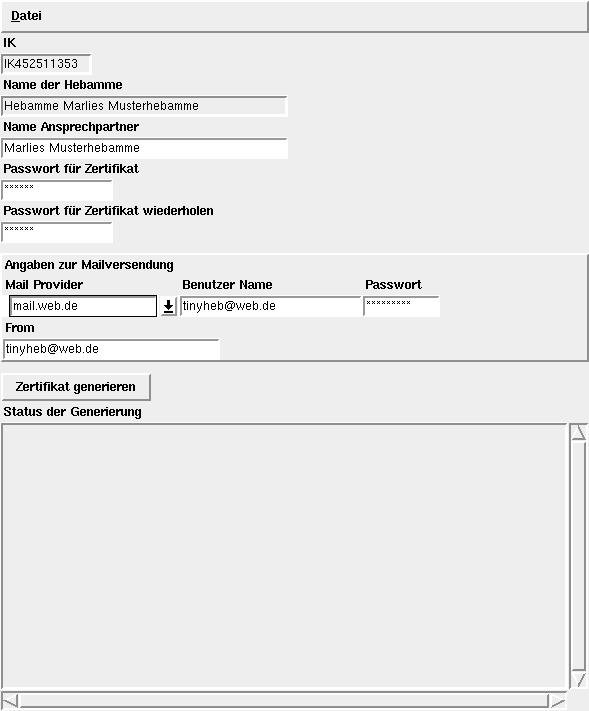
\includegraphics[width=9cm]{certreq}
\caption{\tinyHeb\/ Zertifikatgenerierung\label{zertifikat:fig}}
\end{figure}

\begin{description}
\item[IK]
In dieses Feld wird die IK Nummer der Hebamme aus der \tinyHeb\/ 
Datenbank geschrieben. Das Feld lässt sich nicht ändern. Wer es ändern
möchte, muss dies über die Maske ``Angaben zur Hebamme'' machen.
\item[Name der Hebamme]
In dieses Feld wird der Name der Hebamme, wie er in der \tinyHeb\/
Datenbank hinterlegt ist geschrieben. Das Feld lässt sich nicht ändern. 
Wer es ändern möchte, muss dies über die Maske ``Angaben zur Hebamme'' machen.
Die Bezeichnung Hebamme wird automatisch voran gestellt. Dies lässt sich
nicht ändern.
\item[Name Ansprechpartner]
Hier muss ein Ansprechpartner hinterlegt werden. Im Zweifel ist dies die
Hebamme selbst.
\item[Passwort für Zertifikat]
Hier ist nicht das Passwort des Zertifikates hinterlegt, sondern
das Passwort zu dem entsprechenden privaten Schlüssel. Dieses Passwort
muss man sich sehr gut merken. Es wird später zum Signieren der Rechnungen
benötigt.
\index{Signatur}
\marginline{\Huge\bfseries!}%
\item[Passwort für Zertifikat wiederholen]
Identisch zum Feld \feld{Passwort für Zertifikat}
\item[Angaben zur Mailversendung]
Hier sind die identischen Angaben zu machen, wie bei der elektronischen
Versendung von Rechnungen. Sobald ein Mail Provider ausgewählt wird, 
werden die Felder \feld{Benutzer Name, Passwort} und \feld{From} gefüllt. 
Woher diese
Informationen kommen und wie zusätzliche Provider hinterlegt werden
können ist in Kapitel \vref{anhang:provider} beschrieben.
\end{description}

Durch Klicken des Knopfes \knopf{Zertifikat generieren} wird die Generierung
mit den oben gemachten Angaben gestartet.

Während der Generierung der Zertifikatsanfrage werden einige Fragen gestellt:
\begin{description}
\item[Es existiert schon eine Zertifikatsanfrage, soll diese überschrieben
werden?]
Falls man schon ein Zertifikat besitzt, dieses aber abgelaufen ist, sollte
man die Frage mit 'Ja' beantworten. Hat man schon eine Zertifikatsanfrage
generiert, diese aber nicht an die ITSG per Mail geschickt, kann man diese
Frage mit 'ja' beantworten. 

In allen anderen Fällen sollte man genau
überlegen was man tut und ggf. in der \tinyHeb\/ Mailingliste nachfragen.

\item[Es existiert schon ein privater Schlüssel, soll ein neuer generiert
werden?]
Falls man schon über einen privaten Schlüssel verfügt und keinen neuen
generieren möchte, muss man diese Frage mit 'Nein' beantworten. In diesem
Fall ist zu beachten, das im Feld \feld{Passwort für Zertifikat} des
Passwort des existierenden Schlüssels angegeben wird. 

Falls ein neuer
Schlüssel generiert werden soll, kann oder sollte ein neues Passwort vergeben
werden.

\item[Soll eine verschlüsselte Sicherung des Passwortes angelegt werden?]
Wer sich sicher ist, dass er niemals das Passwort seines privaten Schlüssels
vergisst, kann diese Frage mit 'nein' beantworten. Falls man das Passwort
trotzdem vergisst, muss ein neues Zertifikat beantragt werden.

Wenn die Frage mit 'ja' beantwortet wird, wird eine eine verschlüsselte
Kopie des Passwortes angelegt. Diese Kopie kann nur vom Author von 
\tinyHeb\/ entschlüsselt werden und dies nur dann, wenn diesem die Kopie 
zugeschickt wird. Es ist zu hoffen, dass nie ein Nutzer diese ``Service''
in Anspruch nehmen muss.

\end{description}

Im Rahmen der Generierung werden verschiedene Statusmeldungen erstellt.
Wichtig ist die MD5 Signatur, die auch Prüfsumme, Komprimat des Schlüssels
\marginline{\Huge\bfseries!}%
oder Fingerprint genannt wird. Diese Ziffernfolge ist unterschrieben an
die ITSG zu schicken. Im konkreten Fall wäre dies:
\index{Prüfsumme}
\verb|fd:7a:0f:07:e5:90:0f:er:a5:f2:35:53:25:e6:02:2b|.

\begin{description}
\item[Soll das Zertifikat per E-Mail an die ITSG geschickt werden?]
Diese Frage sollte mit 'Ja' beantwortet werden.

\item[Soll ich die Dateien in die korrekten Verzeichnisse kopieren?\\
 Alte Zertifikate werden überschrieben]
Auch diese Frage sollte mit 'Ja' beantwortet werden. Eine Ausnahme ist nur
gegeben, wenn man schon über ein Zertifikat verfügt und dieses noch nicht 
abgelaufen ist. Dieser Sachverhalt sollte eigentlich nicht vorkommen, da man
sein Folgezertifikat erst dann bestellen sollte, wenn das alte Zertifikat
ungültig geworden ist.
\end{description}


An dieser Stelle sollte eine Sicherung des Verzeichnisses 
\verb|$HOME/.tinyheb/|\footnote{unter Windows im Verzeichnis \textbackslash tinyheb}
durchgeführt und an einem \textbf{sehr} sicheren Ort
verwahrt werden, falls z.B. nach einem Systemabsturz der private
Schlüssel wieder für \tinyHeb\/ nutzbar gemacht werden soll.
\marginline{\Huge\bfseries!}%

Damit ist Schritt eins erledigt.

\begin{figure}[H]
\centering
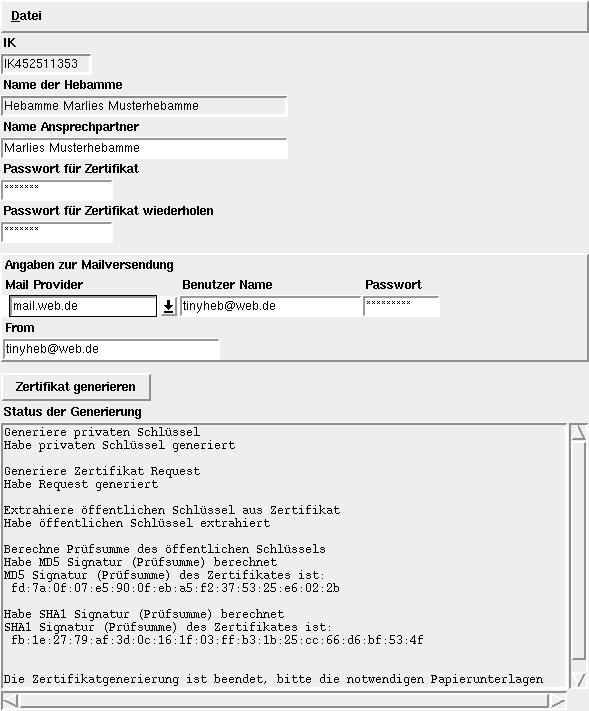
\includegraphics[width=9cm]{certreq2}
\caption{\tinyHeb\/ Zertifikatgenerierung\label{zertifikat2:fig}}
\end{figure}

\subsection{begleitende Unterlagen}
Neben den Unterlagen, die im FAQ der ITSG beschrieben sind, hilft ein
kleines Anschreiben. Es reicht folgendes:
\begin{verbatim}
Hebamme
Marlies Musterhebamme
Strasse
Ort
Tel. 
IK 123456789



Atos Origin GmbH
ITSG Trustcenter
Postach 1225
49702 Meppen

                                                     Ort, den tt.mm.jjjj

Unterlagen zur Zertifikatsanfrage 123456789


Sehr geehrte Damen und Herren,

hier wie von Ihnen gewünscht der unterschriebene Ausdruck des 
öffentlichen Schlüssels / Komprimats:

Komprimat zum Schlüssel (MD5 Hash)
fd:7a:0f:07:e5:90:0f:er:a5:f2:35:53:25:e6:02:2b


Mit freundlichen Grüßen

Marlies Musterhebamme
\end{verbatim}

Das ist alles, was man in Schritt zwei machen muss.

\subsection{Das Zertifikat in \tinyHeb\/ übernehmen}
Sind alle Unterlagen vollständig bei der ITSG eingetroffen, dauert es ein
bis zwei Tage, bis das eigentliche Zertifikat generiert ist. Über diesen
Sachverhalt bekommt man eine Mail, die folgende Betreff Zeile hat:
\verb|12345678.p7c|, d.h., die IK-Nummer der Hebamme ohne Prüfziffer.

Der Dateianhang dieser Mail enthält das eigentliche Zertifikat. Leider 
ist der Anhang \verb|uucoded|, daher habe ich es nicht geschafft, mit
normalen Bordmitteln den Anhang zu lösen. Es gibt in \tinyHeb\/
eine andere Möglichkeit das Zertifikat an der korrekten Stelle abzulegen.

Man lädt sich die Datei \verb|gesamt-pkcs.key| vom FTP Server der ITSG
herunter
\index{gesamt-pkcs.key}
{\href{ftp://trust.itsg.de/dale/}{\nolinkurl{ftp://trust.itsg.de/dale/}}}
und benutzt diese als Eingabe für das Programm \verb|key.pl| 
(siehe auch Anhang \vref{anhang:pubkey}) oder 
\verb|xkey.pl| (seit \tinyHeb\/ Version 1.2.0) aus dem
Verzeichnis \verb|tools|. 

Es ist zu beachten, dass die Datei
\index{gesamt-pkcs.key}
\verb|gesamt-pkcs.key| täglich von der ITSG neu generiert wird, d.h.,
dass eigene Zertifikat ist erst einen Tag nach der Bestätigungsmail in
der Datei enthalten.

\paragraph{Aufruf xkey.pl}
\index{xkey.pl}
\index{eigenes Zertifikat einlesen}
\verb|xkey.pl| kann unter Windows per Doppelklick und unter Linux ganz
normal gestartet werden. Es öffnet sich ein neues Fenster (siehe 
Abbildung \vref{xkey:fig}), in dem verschiedene Angaben zu machen sind.

\begin{figure}[H]
\centering
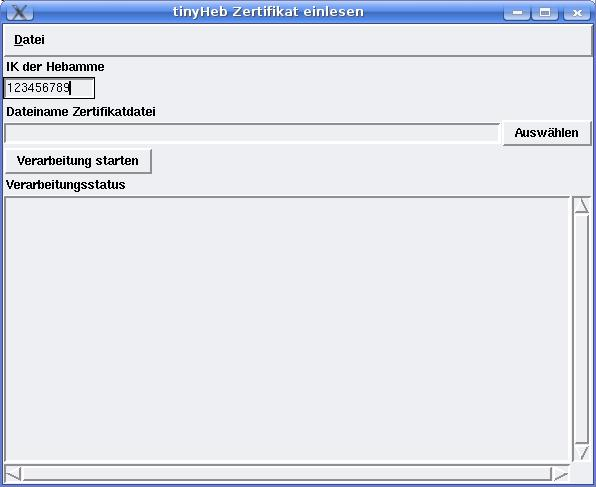
\includegraphics[width=9cm]{xkey}
\caption{\tinyHeb\/ Einlesen des eigenen Zertifikates mit xkey.pl\label{xkey:fig}}
\end{figure}

\begin{description}
\item[IK der Hebamme]
Hier ist die IK Nummer der Hebamme anzugeben, deren Zertifikat übernommen
werden soll. Dieses Feld wird automatisch mit dem Wert aus den Parametern
vorbelegt.
\item[Dateiname der Zertifikatdatei]
Hier ist der Name der Zertifikatdatei anzugeben, in der Regel 
\verb|gesamt-pcks.key|. Über den Knopf \knopf{Auswählen} öffnet sich ein
Dialogfenster, über das der Dateinahme ausgewählt werden kann.
\end{description}

Sind diese beiden Angaben gemacht, kann über den Knopf 
\knopf{Verarbeitung starten} das Einlesen des eigenen Zertifikates
gestartet werden.
Falls das Zertifikat der Hebamme in der Datei enthalten ist, wird es
in das \$HOME Verzeichnis\footnote{unter Windows im Verzeichnis \textbackslash tinyheb\textbackslash privkey} des angemeldeten Benutzers kopiert.
Im Rahmenn Verarbeitungsstatus wird dies angezeigt.
\begin{verbatim}
Habe Zertifikat fuer 123456789 nach /home/xx/.tinyheb/privkey/123456789.pem 
kopiert.
\end{verbatim}
Das Einlesen kann in Abhängigkeit der Rechnerausstattung einige Zeit 
in Anspruch nehmen, da ca. 8000 Zertifikate verarbeitet werden müssen
\footnote{unter Linux kann die Verarbeitung erheblich beschleunigt werden,
indem man das Modul Crypt::OpenSSL::X509 installiert}

\paragraph{Aufruf key.pl}
\verb|key.pl| muss dann mit folgenden Parametern aufgerufen werden:
\\
\verb|key.pl -c -f gesamt-pkcs.key|\footnote{Der Aufruf funktioniert
natürlich nur dann, wenn man vorher die Datei gesamt-pkcs.key im
Verzeichnis tools gespeichert hat}\\
\\
Falls das Zertifikat der Hebamme in der Datei enthalten ist, wird es
in das \$HOME Verzeichnis\footnote{unter Windows im Verzeichnis \textbackslash tinyheb\textbackslash privkey} des angemeldeten Benutzers kopiert.
\begin{verbatim}
Habe Zertifikat fuer 123456789 nach /home/xx/.tinyheb/privkey/123456789.pem 
kopiert.
\end{verbatim}

Damit ist das Zertifikat in \tinyHeb\/ verfügbar und die Rechnungen können
mit einer Signatur versehen werden. Damit dies auch wirklich passiert,
muss der Parameter Signatur der einzelnen Datenannahmestellen auf 
PKCS\#7 Signatur gestellt werden 
(siehe Kapitel \vref{datenannahmestellen:abs}). 
Zukünftig wird \tinyHeb\/ nach dem
Passwort fragen, wenn die Rechnungen verschickt werden.

An dieser Stelle sollte unbedingt eine Sicherung des Verzeichnisses 
\verb|$HOME/.tinyheb/privkey/|\footnote{unter Windows im Verzeichnis \textbackslash tinyheb\textbackslash privkey}
durchgeführt und an einem \textbf{sehr} sicheren Ort
verwahrt werden, falls z.B. nach einem Systemabsturz der private
Schlüssel wieder für \tinyHeb\/ nutzbar gemacht werden soll.
\marginline{\Huge\bfseries!}%



\chapter{Hintergrundinformationen}

In diesem Kapitel sind einige Hintergrundinformationen aufbereitet, die
die Fehlersuche oder auch das Verständnis für die Abläufe in \tinyHeb\/
erleichtern.

\section{Generierung von elektronischen Rechnungen}

In diesem Abschnitt wird beschrieben, wie eine elektronische Rechnung
generiert wird, auf welche Daten zugegriffen wird und welche
Zwischendateien generiert werden.

\paragraph{Voraussetzungen}
Um eine elektronische Rechnung generieren zu können, ist es für \tinyHeb\/
notwendig, dass eine Papierrechnung existiert, d.h. die einzelnen
Rechnungspostionen sind mit dem Status 20 und einer Rechnungsnummer
versehen.

Mit dem Programm \verb|xauftrag.pl| werden genau diese Rechnungen zur 
Anzeige gebracht. Dabei ist folgende Einschränkung zu beachten, existiert
zu einer Krankenkasse keine oder keine parametrisierte Datenannahmestelle
wird die Rechnung nicht angezeigt. Existiert kein öffentlicher Schlüssel
\index{Datenannahmestelle!\"offentlicher Schlüssel} zu der Datenannahmestelle wird die Rechnung
nicht angezeigt.

\subsection{Generierung der elektronischen Rechnung}
Die Generierung der elektronischen Rechnung erfolgt in zwei Phasen.
In der ersten Phase wird überprüft, ob eine elektronsche Rechnung
fehlerfrei produziert werden kann.
In der zweiten Phase wird die echte elektronische Rechnung erzeugt.

\paragraph{Phase eins}
In der ersten Phase wird u.a. geprüft, ob folgende Angaben ermittelt werden
können:

\begin{description}
\item[Angaben zur Frau]
Alle notwendigen Daten zur Frau für die eine Rechnung erstellt werden soll,
werden erst jetzt aus der Datenbank gelesen, d.h. es ist möglich
nachträglich Angaben zu ändern, wie z.B. den Versichertenstatus.
\item[Angaben zur Hebamme]
Alle notwendigen Daten zur Hebamme die eine Rechnung erstellt,
werden erst jetzt aus der Datenbank gelesen, d.h. es ist möglich
nachträglich Angaben zu ändern, wie z.B. die E-Mail Adresse.
\item[Angaben zur Krankenkasse]
Alle notwendigen Daten zur Krankenkasse werden erst jetzt aus der Datenbank 
gelesen. Das Lesen der Daten erfolgt auf Basis der IK-Nummer der Krankenkasse,
wie diese zum Zeitpunkt des Speicherns der Papierrechnung in den Stammdaten
der Frau hinterlegt war. D.h. es ist nicht möglich diese IK-Nummer
nachträglich zu ändern.
Abhängige Daten, wie z.B. die IK-Nummer des Kostenträgers oder der
Datenannahmestelle können nachträglich geändert werden\footnote{siehe
dazu Maske Krankenkassendaten}. 
\item[E-Mail Adresse der Datenannahmestelle]
Es wird geprüft, ob eine E-Mail Adresse zur Datenannahmestelle vorhanden ist.
Es wird nicht geprüft, ob die E-Mail Adresse korrekt ist.
\item[Signierung]
Falls die Rechnung signiert werden soll, wird geprüft, ob dies mit den
bisherigen Angaben möglich ist. Dazu zählen der private Schlüssel der
Hebamme, das Passwort zum privaten Schlüssel und  das Zertifikat der Hebamme.
\item[Verschlüsselung]
Falls die Rechnung signiert werden soll, wird geprüft, ob dies mit den
bisherigen Angaben möglich ist. Dazu zählen der öffentliche Schlüssel
der Datenannahmestelle und eine korrekte OpenSSL Installation.
\end{description}

Folgende Zwischendateien werden während der ersten Phase im Verzeichnis
\$HOME/.tinyheb/tmp/\footnote{unter Windows im Verzeichnis \textbackslash tinyheb\textbackslash tmp}
generiert:
\begin{description}
\item[zik.pem]
In dieser Datei wird der öffentliche Schlüssel der Datenannahmestelle
gespeichert. Wer sich diesen Schlüssel in Klartext ansehen möchte, kann
dies mit OpenSSL machen:
\verb|openssl x509 -in zik.pem -text|
\item[test\_enc]
In dieser Datei sind die unverschlüsselten Nutzdaten der Rechnung enthalten.
\item[test\_enc.sig]
In dieser Datei sind die signierten Nutzdaten der Rechnung enthalten. Falls
die Daten nicht signiert wurden, ist diese Datei identisch zur Datei
\verb|test_enc|. Wer sich die signierten Daten im ASN.1 Format ansehen
möchte, kann dies mit OpenSSL machen: 
\verb|openssl asn1parse -in test_enc.sig -inform DER -dump|
\item[test\_enc.enc]
In dieser Datei sind die verschlüsselten Nutzdaten der Rechnung enthalten.
Falls die Daten nicht verschlüsselt wurden, ist diese Datei identisch zur
Datei \verb|test_enc.sig|. Wer sich die signierten Daten im ASN.1 Format
ansehen möchte, kann dies mit OpenSSL machen:\\
\verb|openssl asn1parse -in test_enc.enc -inform DER -dump|
\end{description}

Mit der Generierung der oben beschriebenen Dateien ist Phase eins der
Rechnungsgenerierung abgeschlossen.


\paragraph{Phase zwei}
In Phase zwei werden ähnliche Dateien wie in Phase eins beschrieben erzeugt.
Allerdings werden in Phase zwei die korrekten Datenaustauschreferenzen und
der korrekte Dateiname genutzt.

Der Dateinahme beginnt entweder mit TSOL oder mit ESOL. 

\index{\textbf{TSOL}}
TSOL, falls die Rechnung im Testbetrieb oder der Eprobungsphase 
übermittelt werden soll.

\index{\textbf{ESOL}}
ESOL, falls die Rechnung im Echtbetrieb übermittelt wird.

Danach folgt eine 4-stellige laufende Nummer, bei dieser Nummer handelt es
sich um die Datenaustauschreferenz (siehe \vref{datenannahmestellen:abs}),
so ensteht zum Beispiel der Dateiname \verb|TSOL0009|. Diese Datei enthält die
Nutzdaten der Rechnung. Die Datei \verb|TSOL0009.sig| enthält die signierten
Nutzdaten, \verb|TSOL0009.enc| die verschlüsselten Nutzdaten. Die Datei 
\verb|TSOL0009.AUF| enthält die Auftragsdaten zu dieser Rechnung.

Nachdem diese Dateien im Verzeichnis \$HOME/.tinyheb/tmp/\footnote{unter Windows im Verzeichnis \textbackslash tinyheb\textbackslash tmp}
generiert wurden und die Rechnung erfolgreich über das Internet 
verschickt werden konnte, werden diese Dateien in ein Unterverzeichnis 
unterhalb tmp verschoben. Dieses Verzeichnis trägt der Namen (IK-Nummer)
des physikalischen Empfängers der Datei, z.B. 107436557.




\section{Sicherheit in \tinyHeb\/}

In diesem Abschnitt wird beschrieben, wie sicher, resp. unsicher 
\tinyHeb\/ ist und wie man es mit bestimmten Handgriffen sicherer macht.
Es ist vermutlich notwendig ein gewisses technisches Verständnis für dieses
Kapitel mitzubringen.

Die Ausführungen sind nach bestem Wissen gemacht, ersetzen jedoch in 
keinem Fall die Lektüre der entsprechenden Programmdokumentation zum
eingesetzten Betriebssystem\footnote{WinXP, Linux um Beispiele zu nennen}, 
der MySQL Datenbank und dem Webserver Apache.

\paragraph{Sicherheit im Betriebssystem}
Einige Betriebssysteme haben eine integrierte Firewall, wer diese abschaltet,
öffnet Angreifern natürlich Tür und Tor um auf die entsprechenden Dienste
zuzugreifen.\footnote{zu diesen Diensten gehören auch Apache und MySQL}
D.h. für \tinyHeb\/ wer keine Firewall hat, der könnte ein Problem mit
der Sicherheit seiner Daten bekommen.
Wer eine Firewall hat, der muss für \tinyHeb\/ die Ports 80 für Apache und
3306 für MySQL für den Zugriff von aussen -- aus dem Internet und/oder
ggf. des LANs -- schließen.

Von Interesse für \tinyHeb\/ ist noch die Datei \verb|privkey.pem| in
der der private Schlüssel zum Signieren von Rechnungen enthalten ist.
Diese Datei sollte nur und ausschließlich Leserechte für den Benutzer
haben, der diese benötigt um Rechnungen zu signieren. 
Damit die Datei nicht versehentlich gelöscht wird,
sollte kein Benutzer Schreibrechte für diese Datei besitzen.


\paragraph{Sicherheit des Webservers}
Der Apache ist ein vollständiger Webserver, der für die Nutzung von
\tinyHeb\/ benötigt wird, d.h. es ist keine Verbindung zum Internet
notwendig, um \tinyHeb\/ Nutzen zu können.

Die Konfigurationsdatei des Webservers enthält für \tinyHeb\/ im Standard
folgende Einstellungen:
\begin{verbatim}
Alias /tinyheb/ "/srv/www/cgi-bin/tinyheb/"

<Directory /srv/www/cgi-bin/tinyheb>
        AllowOverride None
        Options -Indexes +ExecCGI +FollowSymLinks
        AddHandler cgi-script pl
        Order allow,deny
        Allow from all
</Directory>
\end{verbatim}

Mit diesen Einstellungen ist ein Zugriff auf \tinyHeb\/ bei bestehender
Internetverbindung jederzeit möglich! Wenn keine Firewall wie oben 
beschrieben genutzt wird.

Mit folgenden Einstellungen wird die Zugriffsmöglichkeit auf den lokalen
Rechner eingeschränkt:
\begin{verbatim}
Alias /tinyheb/ "/srv/www/cgi-bin/tinyheb/"

<Directory /srv/www/cgi-bin/tinyheb>
        AllowOverride None
        Options -Indexes +ExecCGI +FollowSymLinks
        AddHandler cgi-script pl
        Order deny,allow
        Deny from all
        Allow from 127.0.0.1 
</Directory>
\end{verbatim}

D.h. jetzt kann man sich schon ziemlich sicher sein, dass kein
unbefugter auf die Daten zugreift. 

Wer ganz sicher gehen möchte,
kann einen Passwortschutz für \tinyHeb\/ im Apache hinterlegen.
Wie das geht ist ausführlich im Apache Handbuch im Kapitel
Authentication, Authorization and Access Control beschrieben.


\paragraph{Sicherheit von MySQL}

Wie sicher der Datenbankserver ist, hängt unter anderem davon ab, ob man
für den user root bei der Installation der Datenbank ein Passwort
vergeben hat. Wer ein möglichst kryptisches Passwort vergeben hat, ist
schon mal auf der etwas sicheren Seite, da nur über diesen User
die komplette Datenbank gelöscht werden kann.

Bei der ersten Installation von \tinyHeb\/ wird ein ``\tinyHeb\/'' User
in der Datenbank angelegt, dieser hat den Namen 'wwwrun'@'localhost' und 
wird ohne Passwort angelegt. Mit diesem User ist nur der Zugriff vom
lokalen Rechner möglich. Wenn also Unbefugten Zugriff auf den lokalen
Rechner möglich ist, können diese mit dem User wwwrun Daten aus der
\tinyHeb\/ Datenbank holen. Aber wer sollte dies schon sein?


\paragraph{Sicherheit von tinyHeb}

Es gibt eine echte Sicherheitslücke im \tinyHeb\/ Kern. Wenn über die
Anwendung \verb|xauftrag.pl| Rechnungen signiert werden, wird das
Passwort des Zertifikates im Hauptspeicher gehalten, bis xauftrag.pl
beendet wird. Selbst danach ist es noch möglich, dass sich Reste des
Programms im Speicher befinden, bis dieser Speicherbereich erneut
alloziert wird. D.h. es ist Angreifern möglich, durch Auslesen des 
Hauptspeichers Zugriff auf das Passwort des privaten Schlüssels zu gelangen.

Wenn dann wie oben beschrieben, die Datei privkey.pem öffentlich 
zugänglich ist, können mit der Kombination aus Passwort und privatem
Schlüssel Rechnungen und sonstige E-Mails mit elektronischen Unterschriften
versehen werden.

\paragraph{}
Jeder muss für sich persönlich entscheiden, wie groß sein Sicherheitsbedürfnis
ist. Schließlich leben wir auch privat in Häusern mit ``normalen''
Türen und Schlössern. Wer aber auf große Sicherheit Wert legt, sollte
die obigen Hinweise beachten. 

Dem Author genügt die Firewall für seinen persönlichen Schutz. Die 
Logfiles der Firewall werden allerdings auch täglich kontrolliert.

\bibliography{quellen}
\bibliographystyle{plain}

\printindex
%
\end{document}
